%%%%%%
%%%%%%%%%%%%%%%%%%%%%%%%%%%%%% Title Page Info %%%%%%%%%%%%%%%%%%%%%%%%%%%%%%%%%%%%%%%%%%%
%%%%%%%%%%%%%%%%%%%%%%%%%%%%%%%%%%%%%%%%%%%%%%%%%%%%%%%%%%%%%%%%%%%%%%%%%%%%%%%%%%%%%%%%%%

\documentclass[aspectratio=169,compress]{beamer}
\mode<presentation> 

\usetheme{Warsaw}
\usecolortheme[rgb={0.4,0.0,0.4}]{structure}
%\usecolortheme[rgb={0,0.4,0}]{structure}
%\usetheme{AnnArbor}

% define
%\usepackage{beamerouterthememiniframes} % Para los puntitos 
\setbeamertemplate{footline}[frame number]{}

% include packages
\usepackage{subfigure}
\usepackage{multicol}
\usepackage{amsmath}
\usepackage{epsfig}
\usepackage{graphicx}
\usepackage[all,knot]{xy}
\usepackage{algorithmic}
\xyoption{arc}
\usepackage{url}
\usepackage{multimedia}
\usepackage{hyperref}

\usepackage{pgfpages}
\setbeameroption{hide notes} % Only slides
%\setbeameroption{show only notes} % Only notes
%\setbeameroption{show notes on second screen=right} % Both

\title{Programación de Aplicaciones Móviles Nativas en Android}
%\subtitle{The Beamer Class}
\author{Dr. Marco Aurelio Nu\~no Maganda}
\institute{Universidad Politécnica de Victoria\\ Laboratorio de Sistemas Inteligentes \\
mnunom@upv.edu.mx  \vspace{.25cm} }

\date{Octubre 2024}
%\textbf{nmaganda@ccc.inaoep.mx}


%%%%%%%%%%%%%%%%%%%%%%%%%%%%%%%%%%%%%%%%%%%%%%%%%%%%%%%%%%%%%%%%%%%%%%%%%%%%%%%%%%%%%%%%%%
%%%%%%%%%%%%%%%%%%%%%%%%%%%%%% Begin Your Document %%%%%%%%%%%%%%%%%%%%%%%%%%%%%%%%%%%%%%%
%%%%%%%%%%%%%%%%%%%%%%%%%%%%%%%%%%%%%%%%%%%%%%%%%%%%%%%%%%%%%%%%%%%%%%%%%%%%%%%%%%%%%%%%%%

 

\usepackage[backend=biber,maxcitenames=50,maxbibnames=50,sorting=ydmdddnt]{biblatex}

\DeclareSortingScheme{ydmdddnt}{ 
  \sort{ 
    \field{presort} 
  } 
  \sort[final]{ 
    \field{sortkey} 
  } 
  \sort[direction=descending]{ 
    \field{year} 
  } 
  \sort[direction=descending]{ 
    \field{month} 
  } 
  \sort[direction=descending]{ 
    \field{day} 
  } 
  \sort{ 
    \field{journaltitle} 
  } 
  \sort{ 
    \field{author} 
    \field{editor} 
  } 
  \sort{ 
    \field{title} 
  } 
}




%\renewrobustcmd{\mkbibfootnote}{\normalsize\footnotemark\footnotetext}
\setbeamerfont{footnote}{size=\tiny}






\newcommand{\ArchivoPrincipal}{Todos}
\newcommand{\ArchivoSecundario}{Bibliografia}


%Append keywords to identify different bibliography entries.
\DeclareSourcemap{
  \maps[datatype=bibtex, overwrite]{
    \map{
      \perdatasource{\ArchivoPrincipal.bib}
      \step[fieldset=KEYWORDS, fieldvalue=primary, append]
    }
    \map{
      \perdatasource{\ArchivoSecundario.bib}
      \step[fieldset=KEYWORDS, fieldvalue=secundary, append]
    }    
  }
}


\addbibresource{\ArchivoPrincipal.bib}
\addbibresource{\ArchivoSecundario.bib}

\usepackage{listings}
 
 \AtBeginSection[]
{
    \begin{frame}
        \frametitle{Outline}
        \tableofcontents[currentsection]
    \end{frame}
}

% ACtualizacion 2024: Se necesita esta Entrada
\newcommand{\EntradaBibtex}{InvalidEntry}
\renewcommand*{\thefootnote}{\fnsymbol{footnote}}

\begin{document}

\frame{
	%\titlepage 
	\begin{titlepage}
	\end{titlepage}
	
}

\frame{
\frametitle{Contenido}
\tableofcontents
}


\section[IAyPM]{Introducción a Android y a la Programación Móvil}



\begin{frame}{Programación Móvil}
%\begin{block}{Programación Móvil} 
\begin{columns}
\begin{column}{0.98\textwidth}
    \begin{center}

\begin{itemize}
\item Es la actividad de desarrollar una aplicación específicamente para teléfonos inteligentes.
\item Estas aplicaciones se encuentran preinstaladas en el teléfono o pueden ser instaladas por el usuario mediante una tienda de aplicaciones (App Store o Google Play)
\item Las tareas que tradicionalmente hacíamos en la PC ahora están migrando hacia el teléfono inteligente
\item Principales sistemas operativos móviles: Android, iOS,
\item Enfocados principalmente en el desarrollo de aplicaciones NATIVAS.
\item Lenguajes de programación: Java, Kotlin.
\end{itemize}
     \end{center}

\end{column}
\end{columns}
%\end{block} 
\end{frame}


\begin{frame}
\frametitle{Sistema Operativo}  
\begin{columns}
%\column{0.32\linewidth}
\column{0.65\linewidth}
\begin{block}{}
Un Sistema Operativo (SO) es un programa (software) que al arrancar la computadora** se encarga de gestionar todos los recursos del sistema informático permitiendo así la comunicación entre el usuario y la computadora. 
\end{block}
\begin{center}
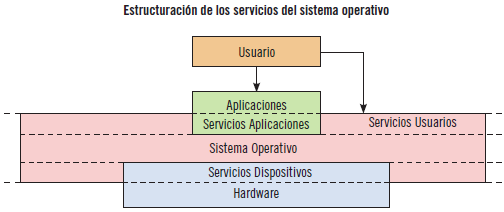
\includegraphics[width=0.95\linewidth]{00_IntroProgramacionYMoviles/SistemaOperativo1.png} 
\end{center}
\tiny{\url{https://reader.digitalbooks.pro/content/preview/books/38230/book/OEBPS/Text/c1.html}}

\column{0.32\linewidth}
\begin{center}
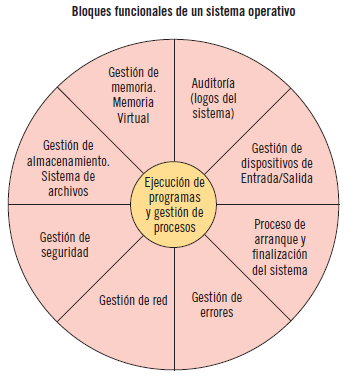
\includegraphics[width=0.95\linewidth]{00_IntroProgramacionYMoviles/SistemaOperativo2.png} 
\end{center}
\end{columns}

\end{frame}


\begin{frame}
\frametitle{Sistemas Operativos para PCs}  

\begin{columns}
\column{0.32\linewidth}
\begin{center}

\includegraphics[width=0.95\linewidth]{00_IntroProgramacionYMoviles/Windows11.png} 
\end{center}

\column{0.32\linewidth}
\begin{center}

\includegraphics[width=0.95\linewidth]{00_IntroProgramacionYMoviles/MacOS.png} 
\end{center}

\column{0.32\linewidth}
\begin{center}

\includegraphics[width=0.95\linewidth]{00_IntroProgramacionYMoviles/Linux.png} 
\end{center}
\end{columns}

\end{frame}





\begin{frame}
\frametitle{Telefono Celular No-inteligente vs Telefono Celular Inteligente}  

\begin{columns}
\column{0.46\linewidth}
\begin{block}{Tel\'efono No-inteligente}
\begin{itemize}
\item Su funcionalidad principal era la comunicaci\'on (llamadas o mensajes) a trav\'es de la red celular (GSM)
\end{itemize}
\end{block}
\begin{block}{Tel\'efono inteligente}
\begin{itemize}
\item Interfaz de entrada: Pantalla Touch (a color, de alta definici\'on) 
\item Conexi\'on a Internet: WiFi, GSM (4G o 5G)
\item Comunicaci\'on con otros dispositivos: Bluetooth, NFC
\item C\'amaras (Frontal y Posterior)
\end{itemize}
\end{block}

\column{0.18\linewidth}
\begin{center}
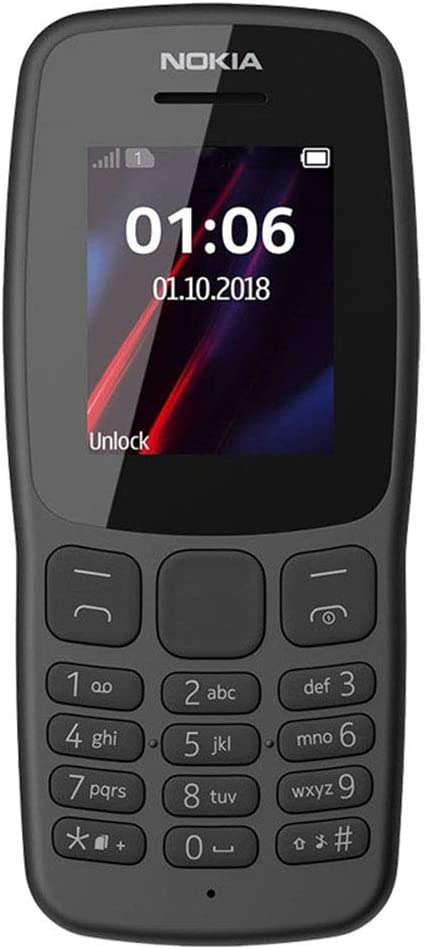
\includegraphics[width=0.95\linewidth]{00_IntroProgramacionYMoviles/FeaturePhone_Nokia.png} 
\end{center}
\column{0.28\linewidth}
\begin{center}
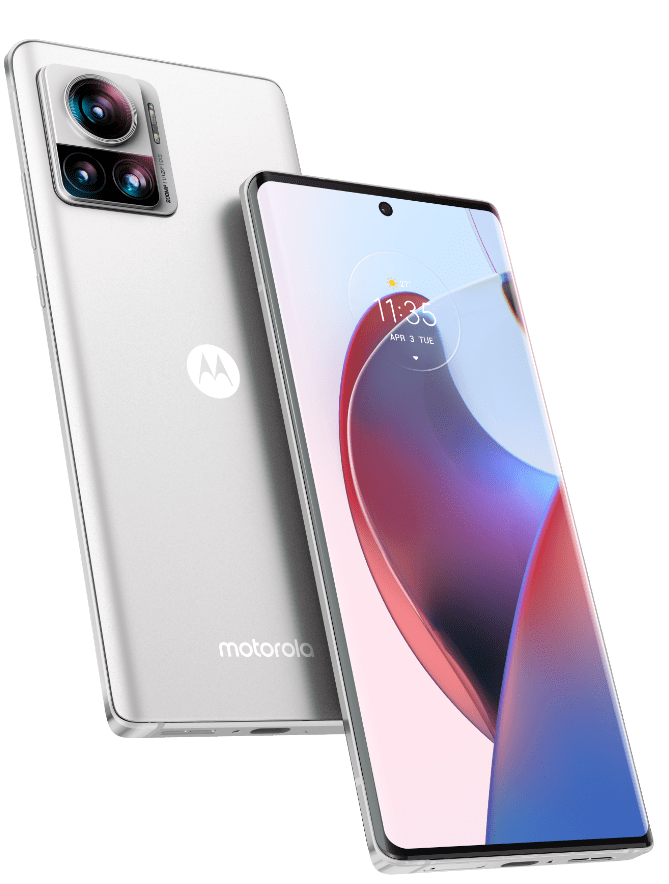
\includegraphics[width=0.95\linewidth]{00_IntroProgramacionYMoviles/Smartphone_Motorola.png} 
\end{center}
\end{columns}
\end{frame}

\begin{frame}
\frametitle{Sistemas Operativos para Telefonos Inteligentes} 
\begin{columns}
\column{0.32\linewidth}
\begin{center}

\includegraphics[width=0.95\linewidth]{00_IntroProgramacionYMoviles/Android.png} 
\end{center}

\column{0.32\linewidth}
\begin{center}
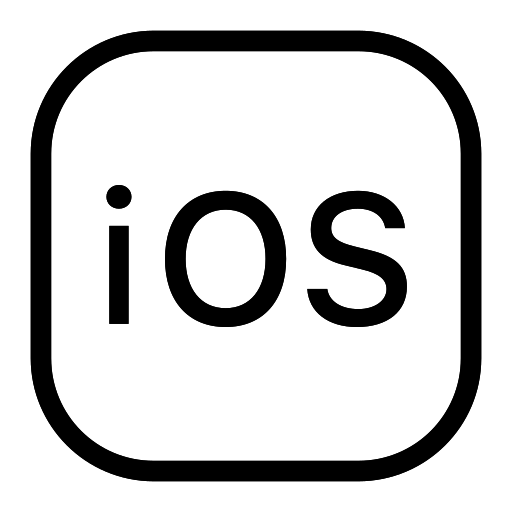
\includegraphics[width=0.95\linewidth]{00_IntroProgramacionYMoviles/iOs.png} 
\end{center}

\column{0.32\linewidth}
\begin{center}

\includegraphics[width=0.95\linewidth]{00_IntroProgramacionYMoviles/WindowsPhone.png} 
\end{center}
\end{columns}
 
\end{frame}


\begin{frame}
\frametitle{Android} 
\begin{columns}
\column{0.64\linewidth}
\begin{itemize}
\item Android es un sistema operativo móvil basado en Linux 
\item Principalmente orientado a dispositivos de pantalla t\'actil (Smartphone, tablets, smartwatches, etc)
\item Fue desarrollado por Android Inc (Adquirida por Google en 2005)
\item Vinculado con un grupo de empresas (HTC, Sony, Motorola, Samsung, LG, Lenovo, entre otras) para la creaci\'on de un SO com\'un para sus dispositivos
\item A la fecha (Q1 2023), los tel\'efonos con SO Android concentran mas del 70\% del mercado global. 
\end{itemize}
\column{0.32\linewidth}
\begin{center}
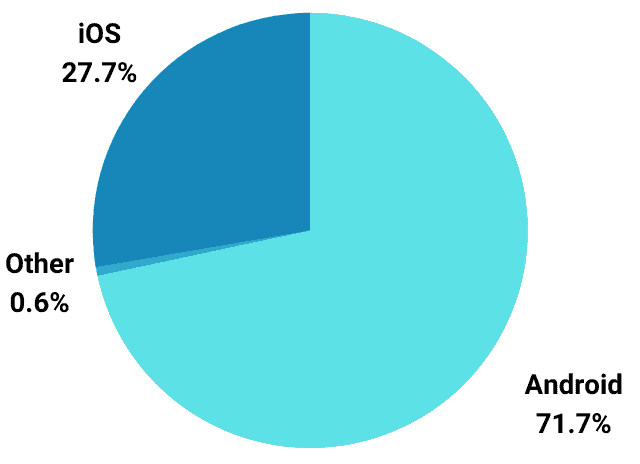
\includegraphics[width=0.95\linewidth]{00_IntroProgramacionYMoviles/AndroidVSIOs_WorldWide.png} 
\end{center}
\end{columns}
 
\end{frame}





\begin{frame}
\frametitle{Aplicaciones Móviles}  
\begin{columns}
\column{0.4\linewidth}
\begin{itemize}
\item Ejecutadas en el tel\'efono
\item La entrada de datos es mediante un teclado ``virtual''
\item El apuntador del raton es la pantalla 
\item Incluyen una interfaz de usuario gr\'afica (GUI) 
\item Es posible descargar miles de \'estas en nuestros dispositivos
\end{itemize}
\column{0.30\linewidth}
\begin{center}
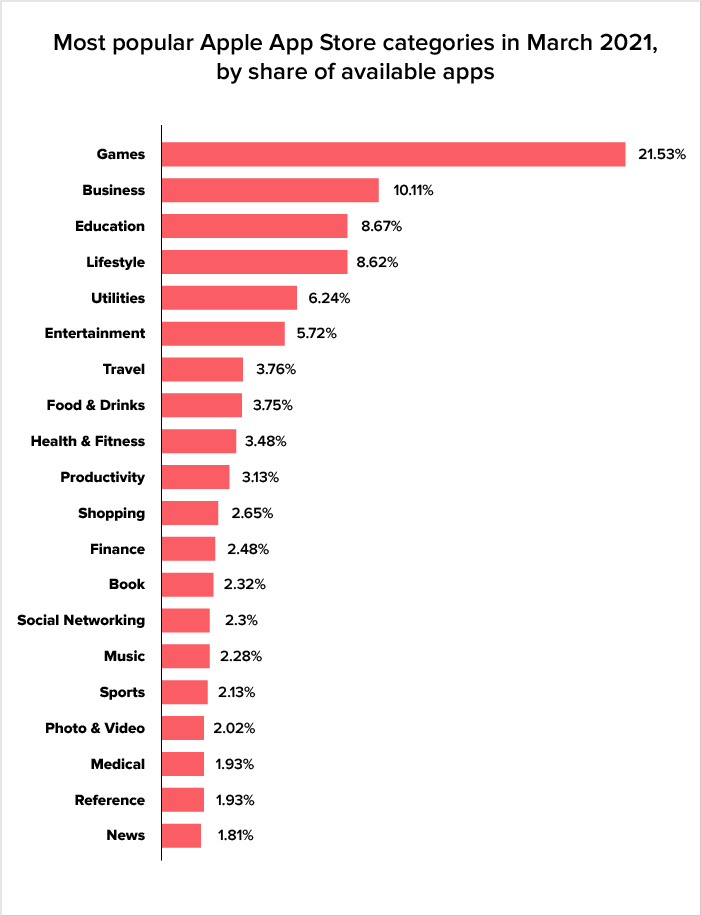
\includegraphics[width=0.95\linewidth]{00_IntroProgramacionYMoviles/TiposAplicaciones.png} 
\end{center}
\column{0.30\linewidth}
\begin{center}
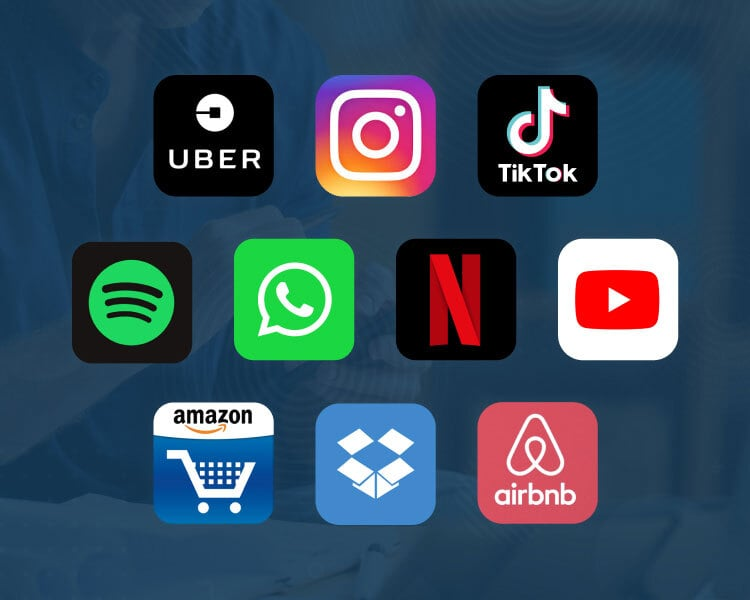
\includegraphics[width=0.95\linewidth]{00_IntroProgramacionYMoviles/most-popular-apps.jpg} 
\tiny{\url{https://www.netsolutions.com/insights/top-10-most-popular-apps-2018/}}  
\end{center}
\end{columns}
\end{frame}


\begin{frame}
\frametitle{Android Studio}  

\begin{itemize}
\item Android Studio es un entorno oficial de desarrollo integrado (IDE) para el sistema operativo Android de Google
\item La primera versi\'on se libera en el año 2013, siendo el lenguaje de programacion Java
\item En 2019, se reemplaza el lenguaje oficial de desarrollo por Kotlin, aunque Java todav\'ia es soportado
\item Es gratis, se puede descargar e instalar en cualquier computadora sin importar el sistema operativo (Windows, Linux y MacOS)
\url{https://developer.android.com}
\end{itemize}
\end{frame}







\section[PAE]{Proyectos aplicados en educación}


\begin{frame}{\citetitle{MarcoNuno_Revista_2020_06_00} \footnotemark (1)}
\begin{block}{Sistema de Monitoreo de Aprendizaje Remoto } 

Con la reciente pandemia, se detectan problemas con el seguimiento del aprendizaje:

	\begin{itemize}
		\item No es posible determinar si el estudiante es quien realiza las tareas
		\item No hay certeza de que tanto tiempo el estudiante dedica a ciertas tareas
	\end{itemize}

Se propone una herramienta cuyos componentes son:
\begin{itemize}
\item Aplicación de Escritorio - El docente asigna tareas·
\item Aplicación en la NUBE - Almacena tareas y evidencias (fotos).
\item Aplicación de Móvil - Monitorea al estudiante emplenado la cámara frontal del teléfono inteligente, además le permite recopilar evidencias.
\end{itemize}
\end{block} 
\footnotetext[1]{\fullcite{MarcoNuno_Revista_2020_06_00}}
\setcounter{footnote}{0}
\end{frame}

\begin{frame}{\citetitle{MarcoNuno_Revista_2020_06_00} (2)}


\begin{columns}
\begin{column}{0.65\textwidth}
\begin{block}{La aplicación de escritorio:} 
		\begin{itemize}
		\item Permite crear grupos, tareas, dar de alta alumnos
		\item Descargar evidencias
		\item Generar una gráfica de tiempo de atención
		\end{itemize}
\end{block} 
\begin{block}{La aplicación móvil:} 
		\begin{itemize}
		\item Recibe las tareas y las muestra al alumno
		\item Monitorea al estudiante a lo largo del desarrollo de sus tareas
		\end{itemize}
\end{block} 
\end{column}
\begin{column}{0.35\textwidth}  
    \begin{center}
     %%%%% this is a minipage, so \textwidth is already adjusted to the size of the column
     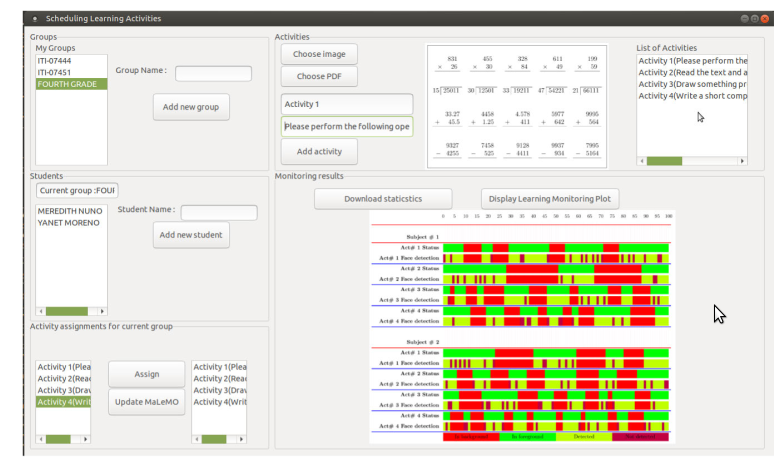
\includegraphics[width=0.95\textwidth]{Figs/LearningMonitoring1}
     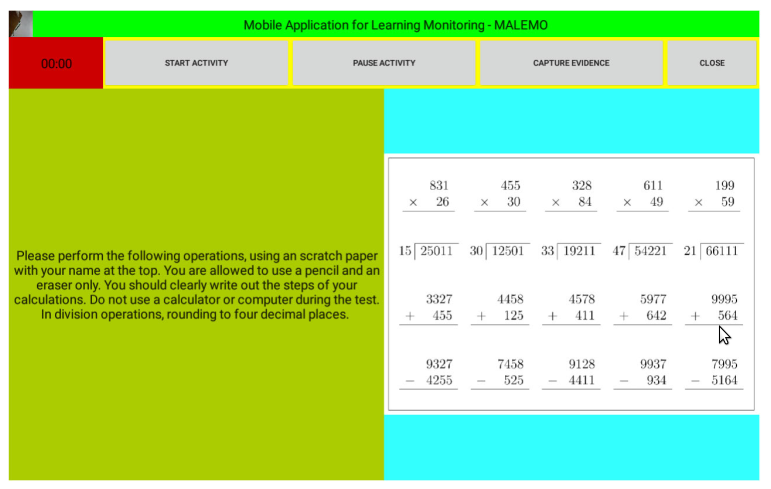
\includegraphics[width=0.95\textwidth]{Figs/LearningMonitoring2}
     \end{center}
\end{column}
\end{columns}


\end{frame}

\begin{frame}{\citetitle{MarcoNuno_Revista_2020_06_00} (3)}


\begin{columns}
\begin{column}{0.5\textwidth}
\begin{block}{Pasos ejecutados por la App: } 
		\begin{itemize}
		\item Detecta la cara del estudiante y estima hacia donde esta mirando (la pantalla, el área de trabajo o el exterior)
		\item Detecta cuando el estudiante cierra la aplicación y lleva la cuenta del tiempo que la aplicación de monitoreo permanece inactiva. 
		\end{itemize}
\end{block} 
	\begin{center}
		 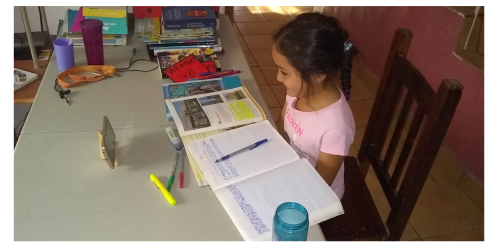
\includegraphics[width=0.50\textwidth]{Figs/LearningMonitoring3}
	\end{center}
\end{column}
\begin{column}{0.5\textwidth}  
    \begin{center}
     %%%%% this is a minipage, so \textwidth is already adjusted to the size of the column
     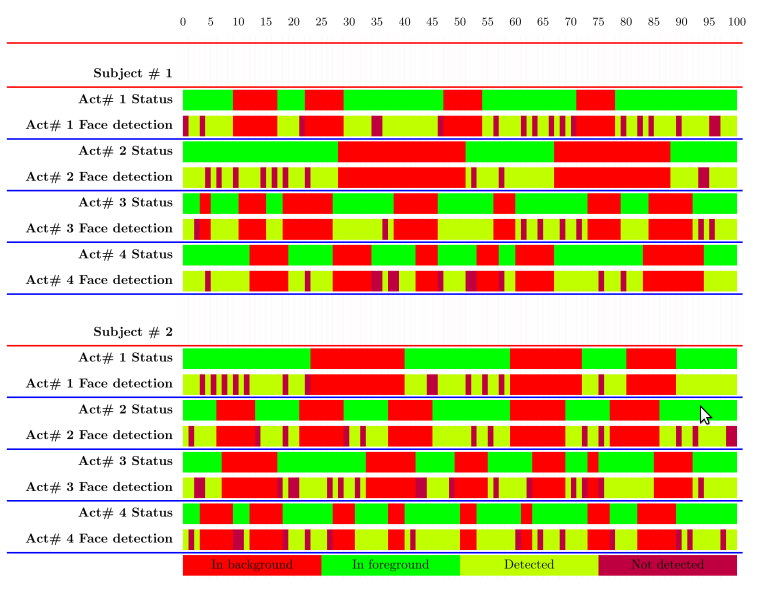
\includegraphics[width=0.99\textwidth]{Figs/LearningMonitoring4}
     \end{center}
\end{column}
\end{columns}

%\end{block} 
\end{frame}


 % Remote Learning (JCR)

\begin{frame}{Aplicación para Pase de Lista (1)}
\begin{block}{Motivación} 
Es necesario una herramienta que permita al profesor pasar asistencia de manera ágil y rápida. 
\begin{itemize}
\item El profesor debe ingresar los grupos a partir de archivos de texto
\item El profesor ingresa a pase de lista y selecciona uno de sus grupos
\item Puede seleccionar asistencia a todos o falta a todos para agilizar el proceso
\item La aplicacion genera un informe con las estadisticas de asistencias, faltas y retartdos
\item Originalmente la lista se manejaba por archivos de texto, despues se migró a una base de datos SQLite
\end{itemize}
\end{block} 
\end{frame}


\begin{frame}{Aplicación para Pasar Lista (2)}
%\begin{block}{Pantallas Principales} 
\begin{center}
	\begin{tabular}{cccc}
		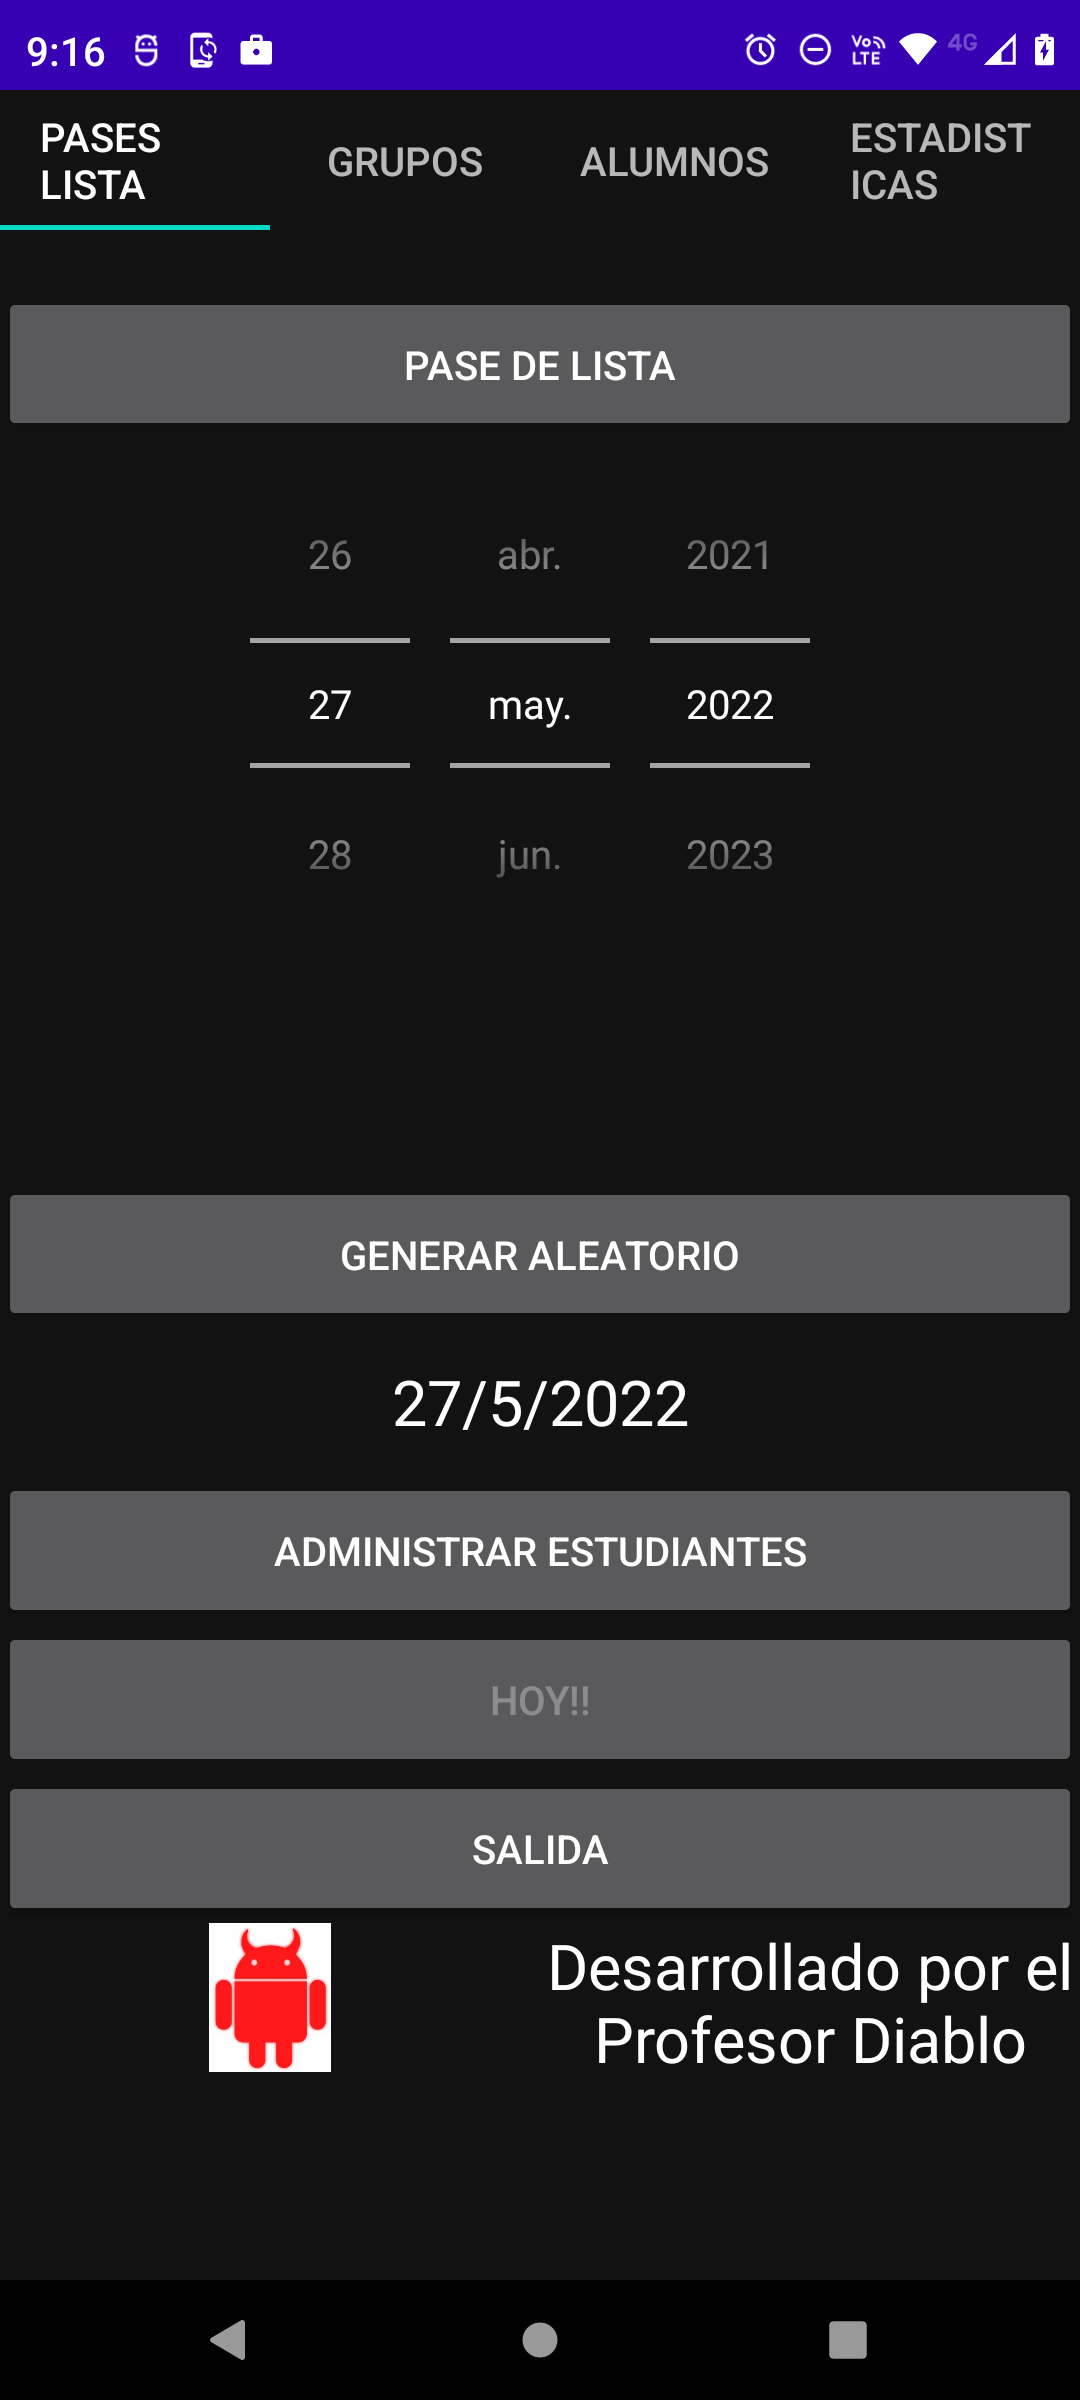
\includegraphics[width=0.20\linewidth]{2022_AppPaseLista/figs/PaseLista0.png} &
		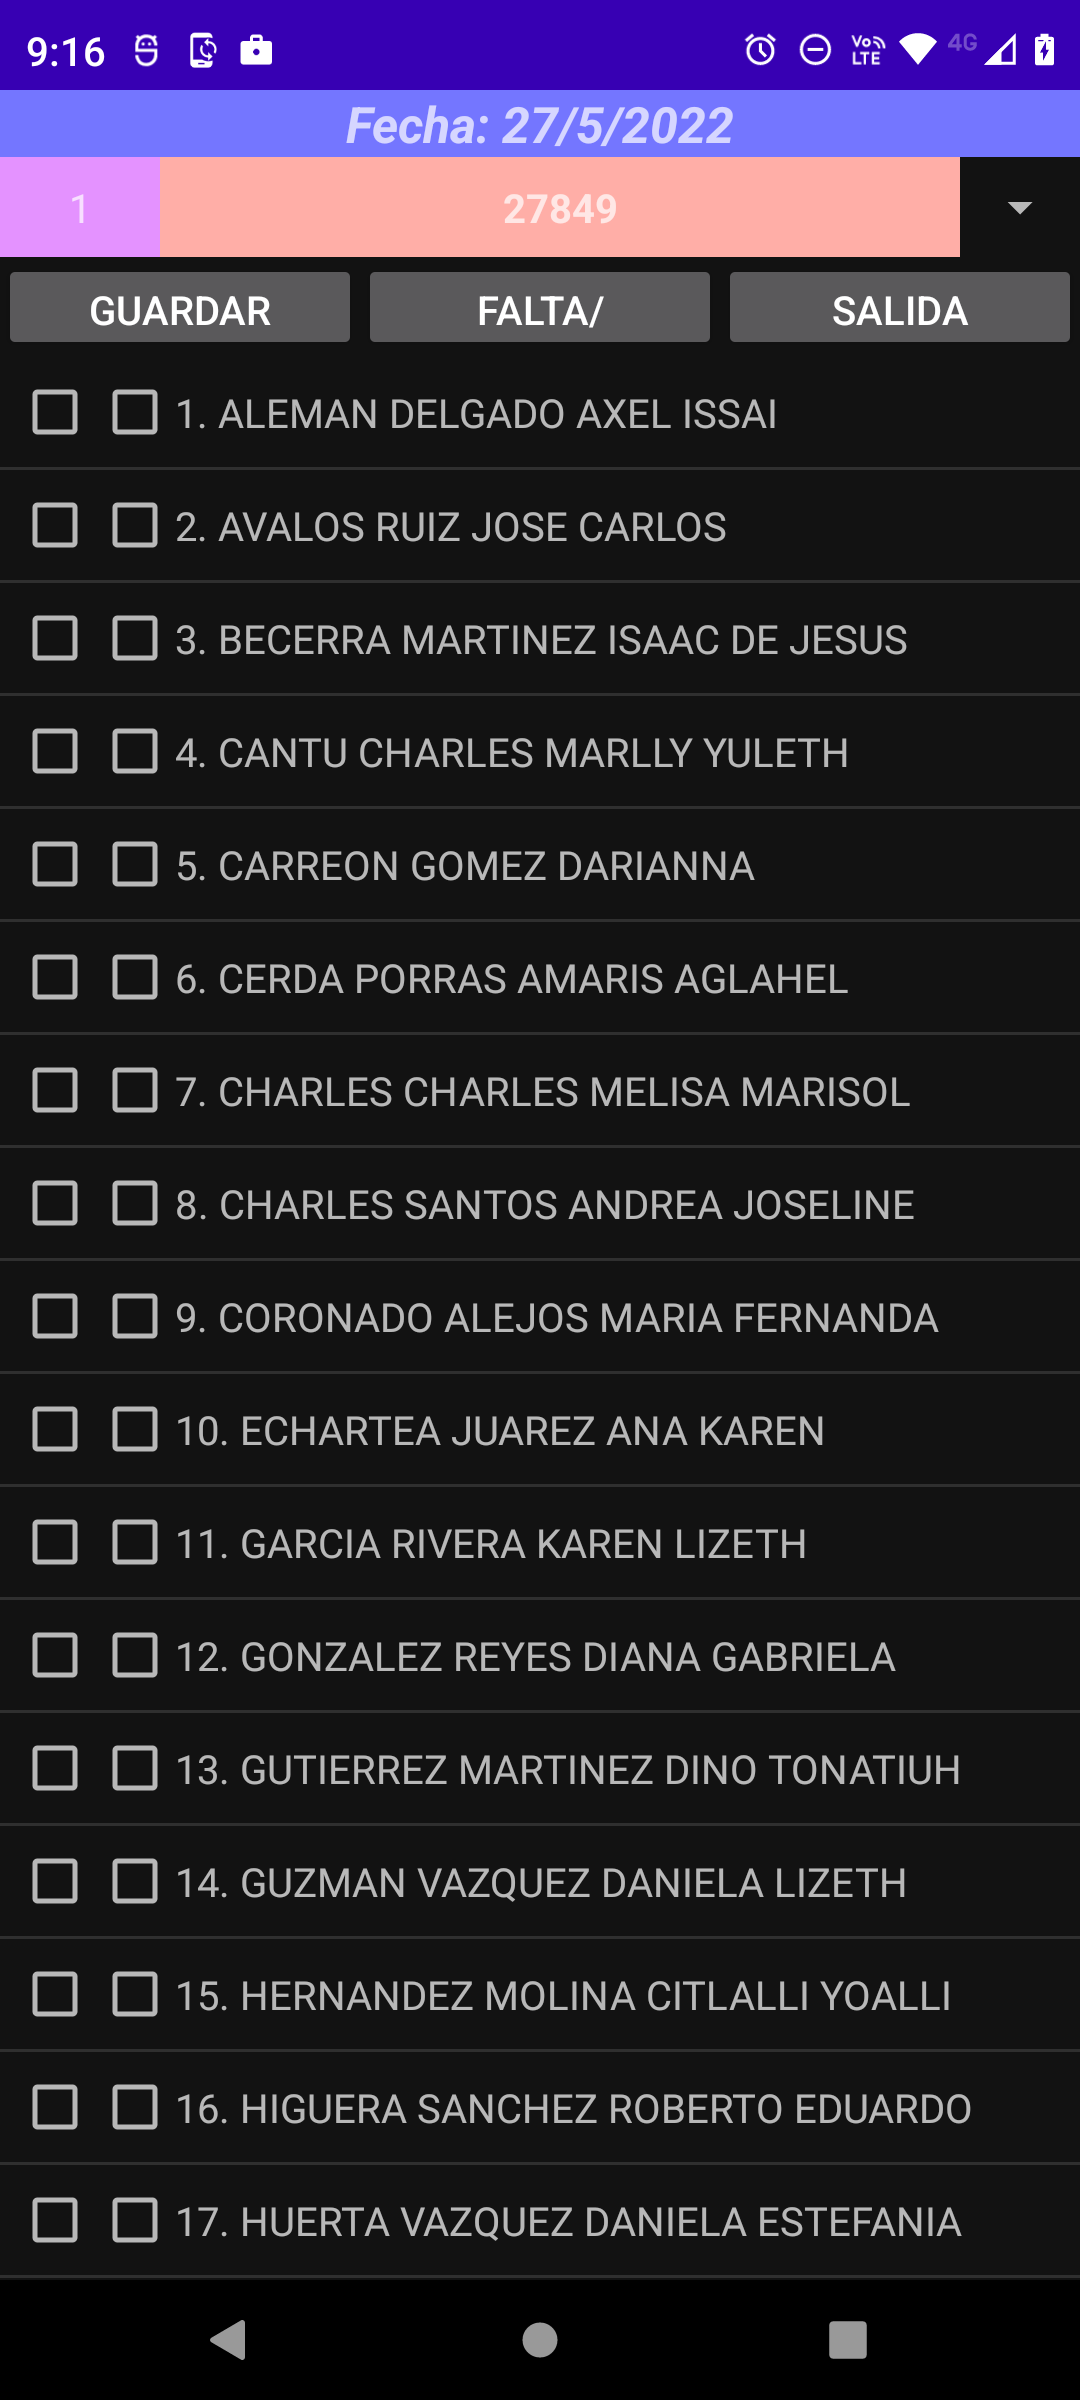
\includegraphics[width=0.20\linewidth]{2022_AppPaseLista/figs/PaseLista1.png} & 		 		
		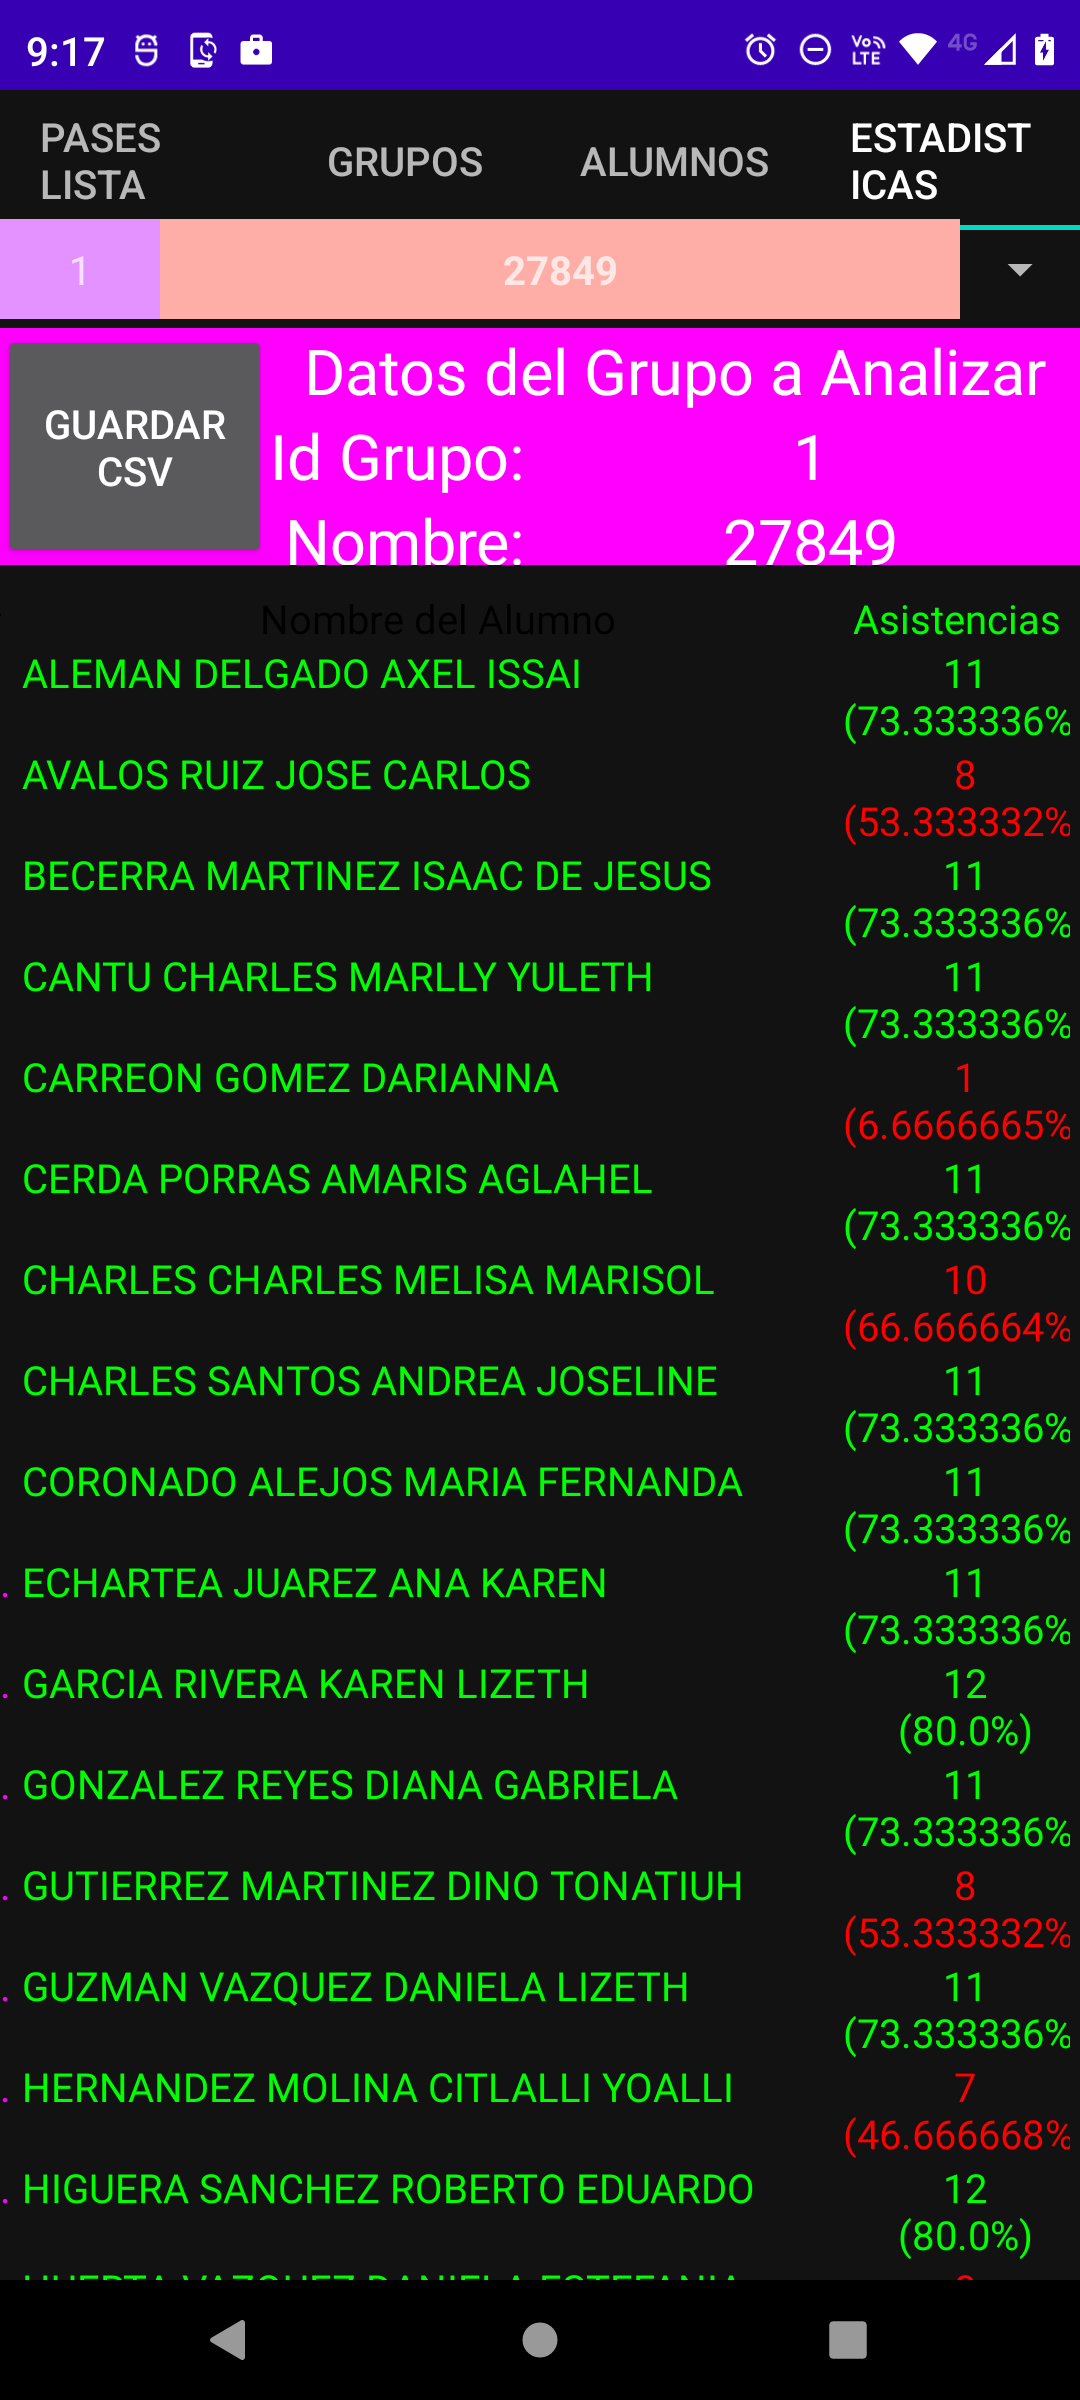
\includegraphics[width=0.20\linewidth]{2022_AppPaseLista/figs/PaseLista2.png} & 		
		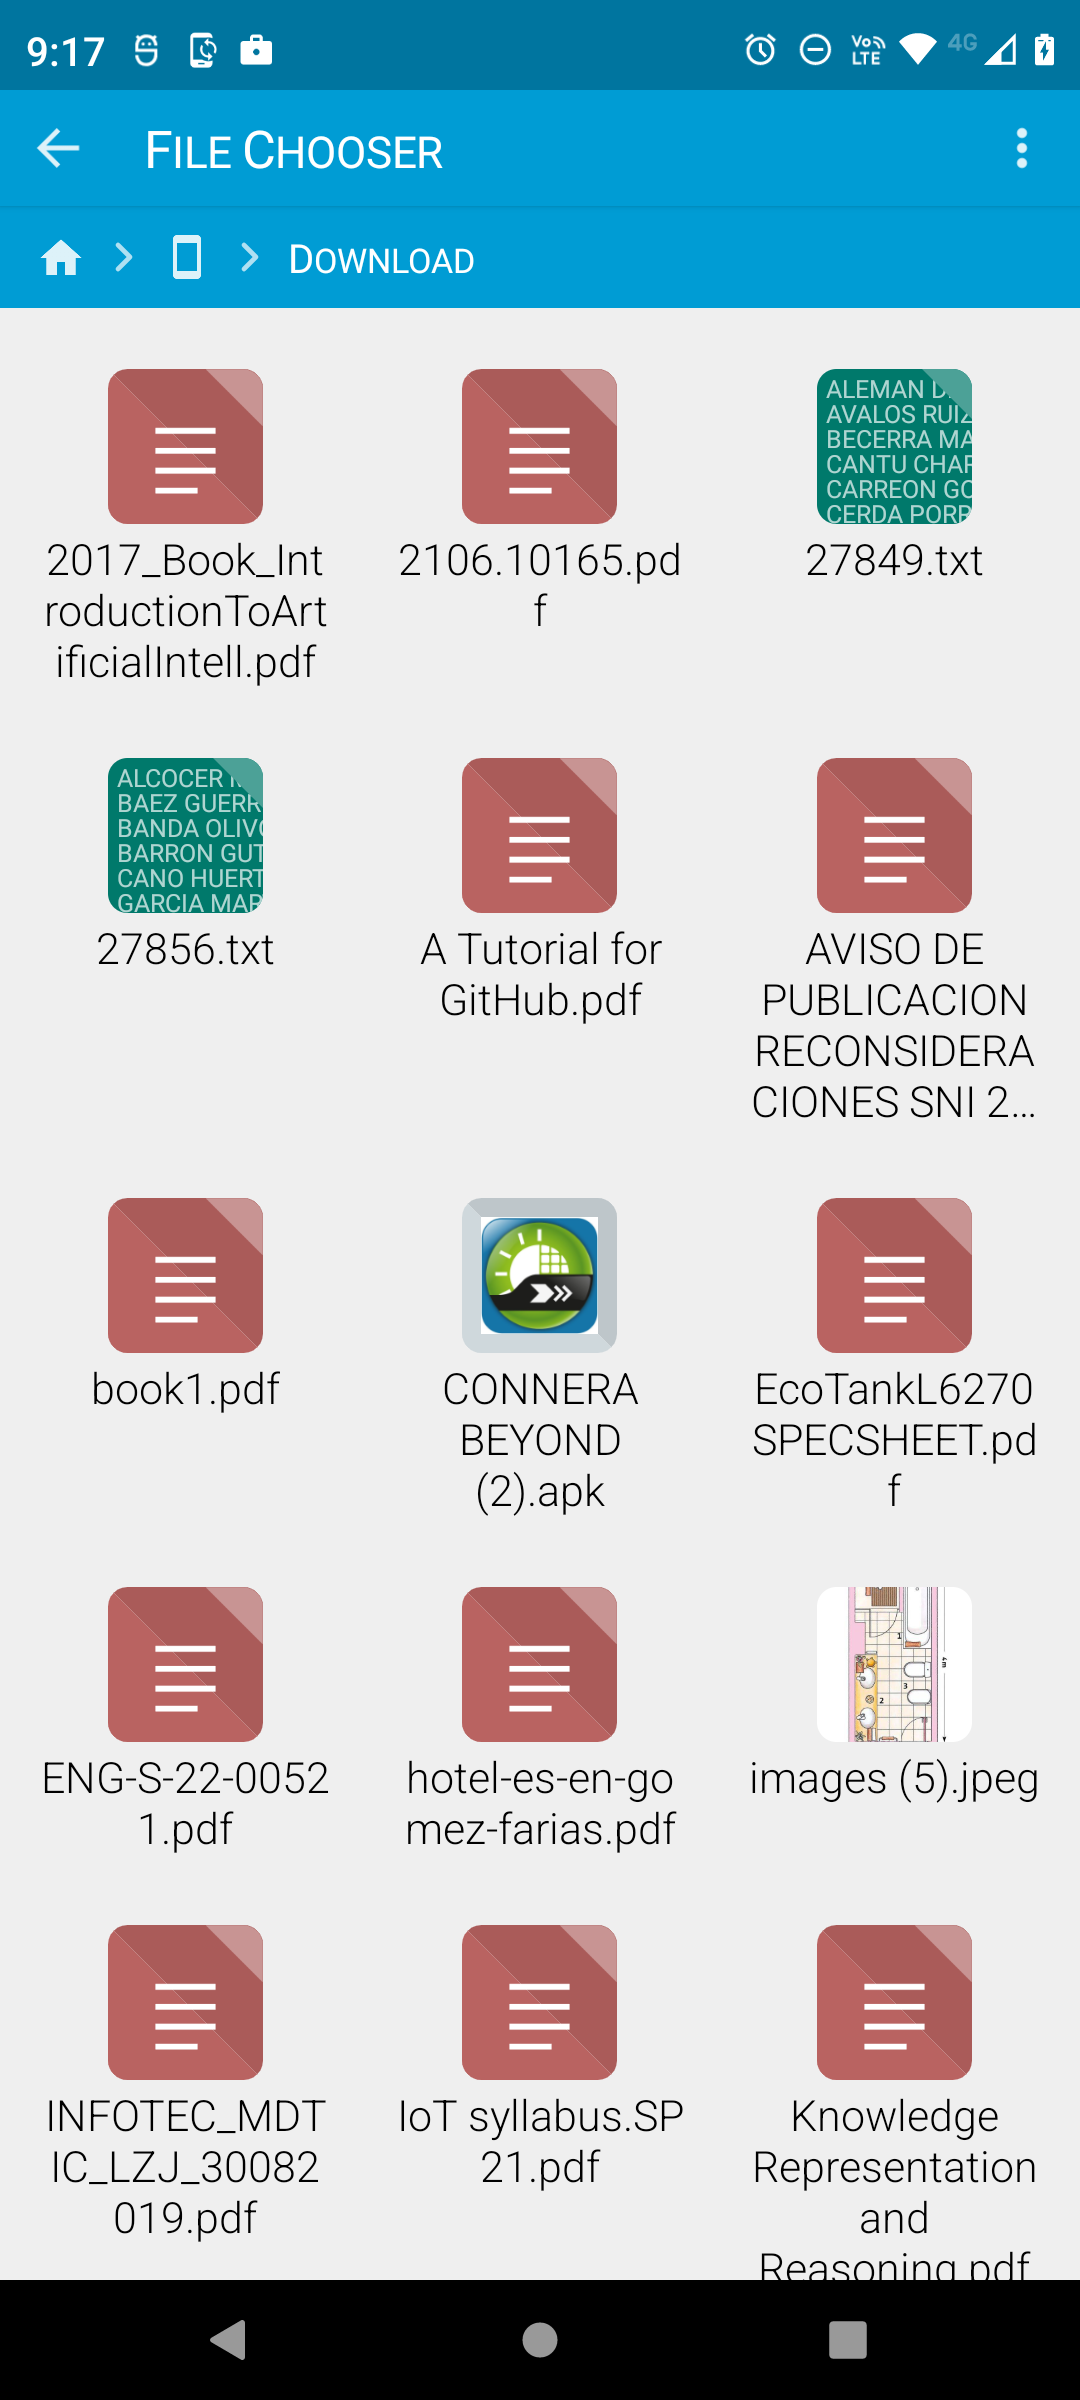
\includegraphics[width=0.20\linewidth]{2022_AppPaseLista/figs/PaseLista3.png} \\
	\end{tabular}
\end{center}
\end{frame}



 % Pase lista

\begin{frame}{Aplicación para entrenamiento de Spelling (1)}
\begin{block}{Motivación} 
Es necesario una herramienta que apoye a los padres a entrenar a sus hijos para concursos de Spelling
\begin{itemize}
\item El usuario ingresa las palabras
\item La aplicacion muestra el deletro de dicha palabra
\item Mediante el sintetizador de voz, es posible leer toda la palabra o el deletreo de la misma para corregir
\item La lista de palabras se va guardando de manera local, no es necesario volver a escribirla
\item Es posible hacer correcciones a las palabras ingresadas
\end{itemize}
\end{block} 
\end{frame}


\begin{frame}{Aplicación para entrenamiento de Spelling (2)}
%\begin{block}{Pantallas Principales} 
\begin{center}
	\begin{tabular}{cc}
		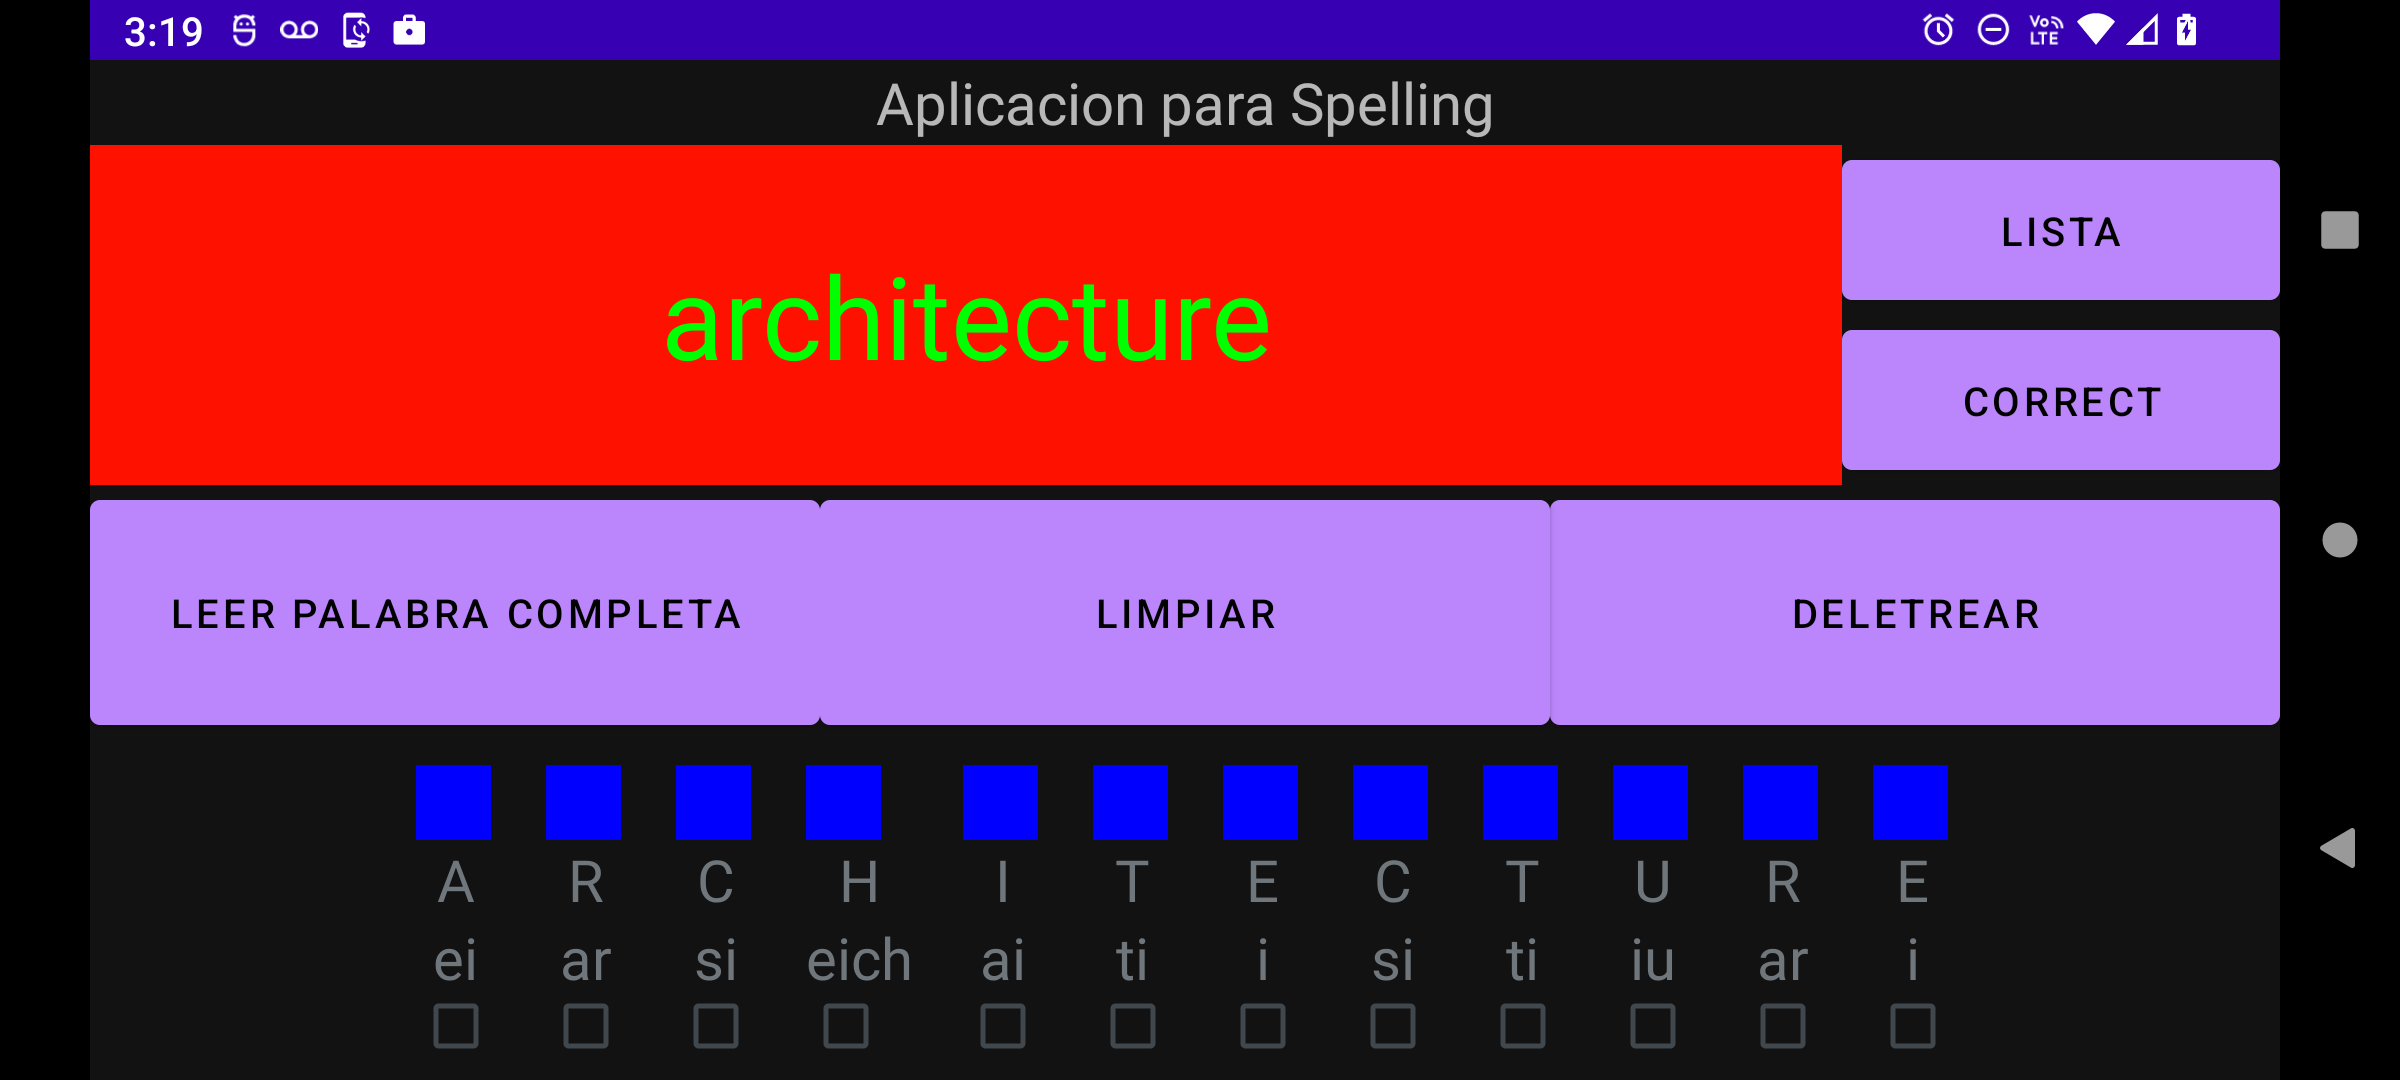
\includegraphics[width=0.46\linewidth]{2022_Spelling/figs/Spelling0.png} &
		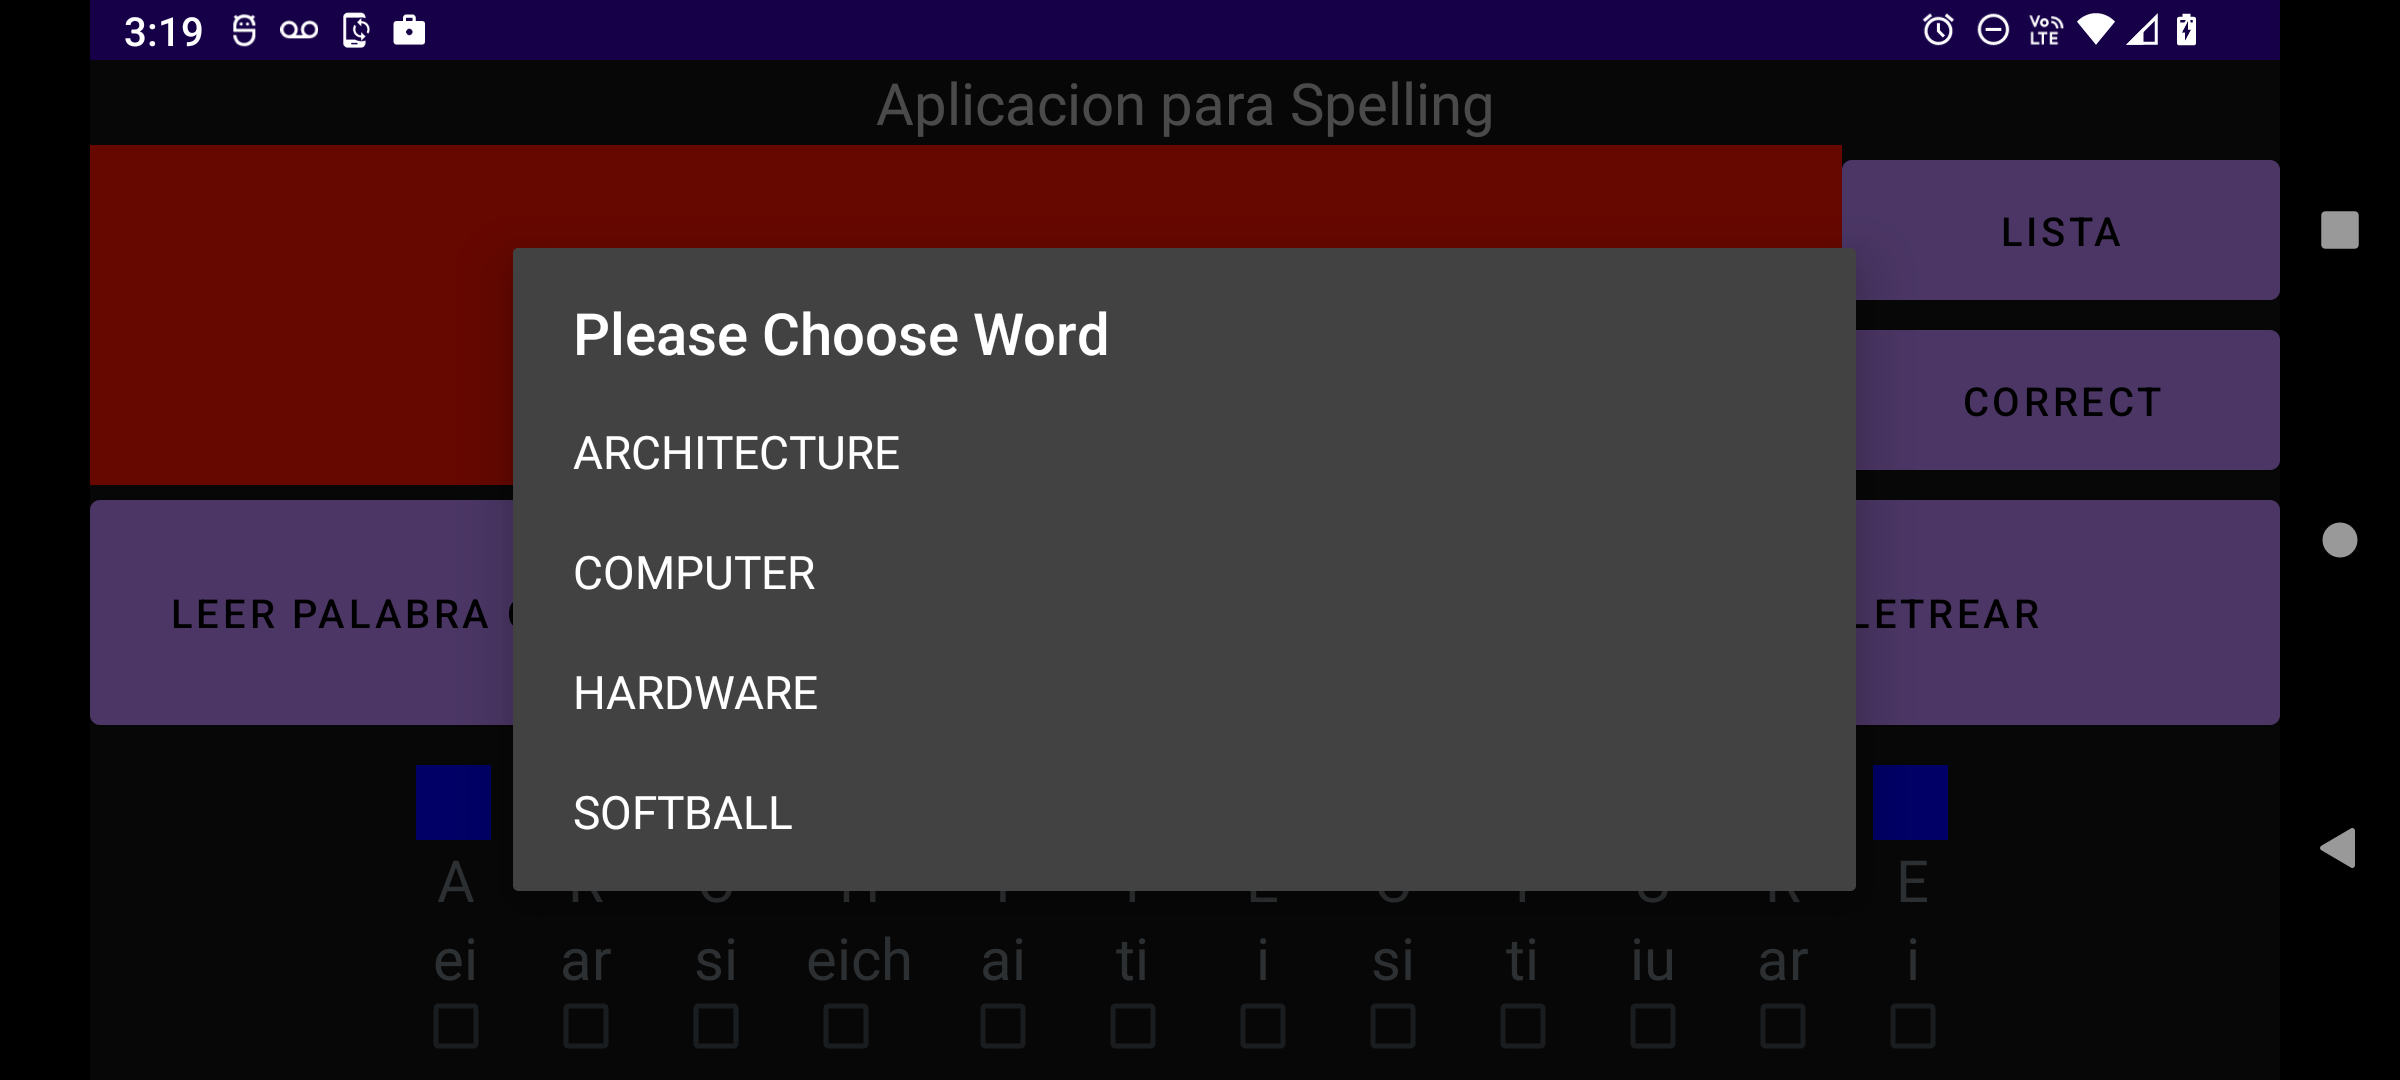
\includegraphics[width=0.46\linewidth]{2022_Spelling/figs/Spelling1.png} \\ 		 		
		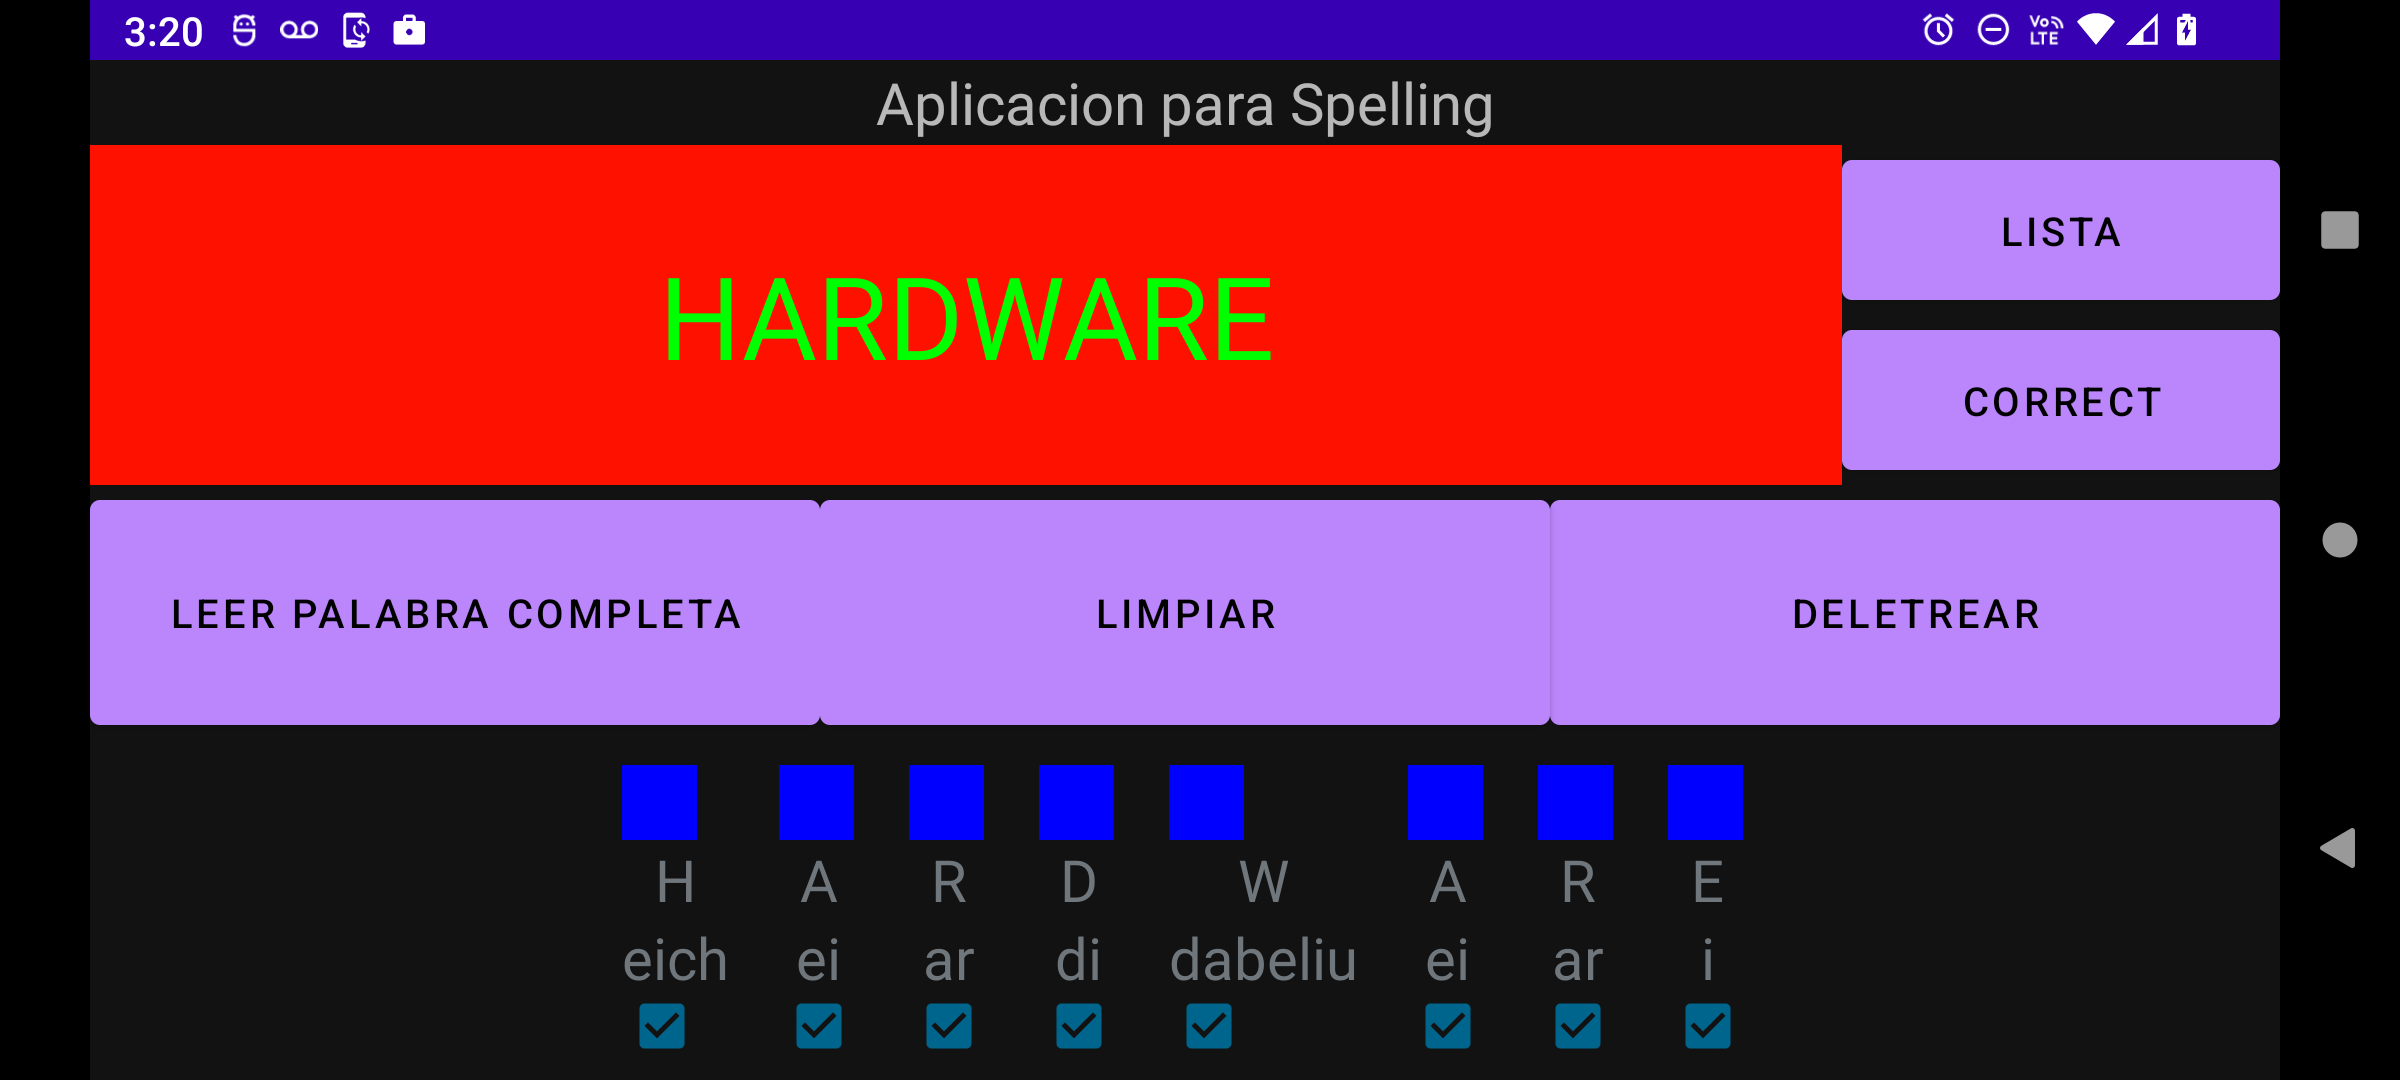
\includegraphics[width=0.46\linewidth]{2022_Spelling/figs/Spelling2.png} & 		
		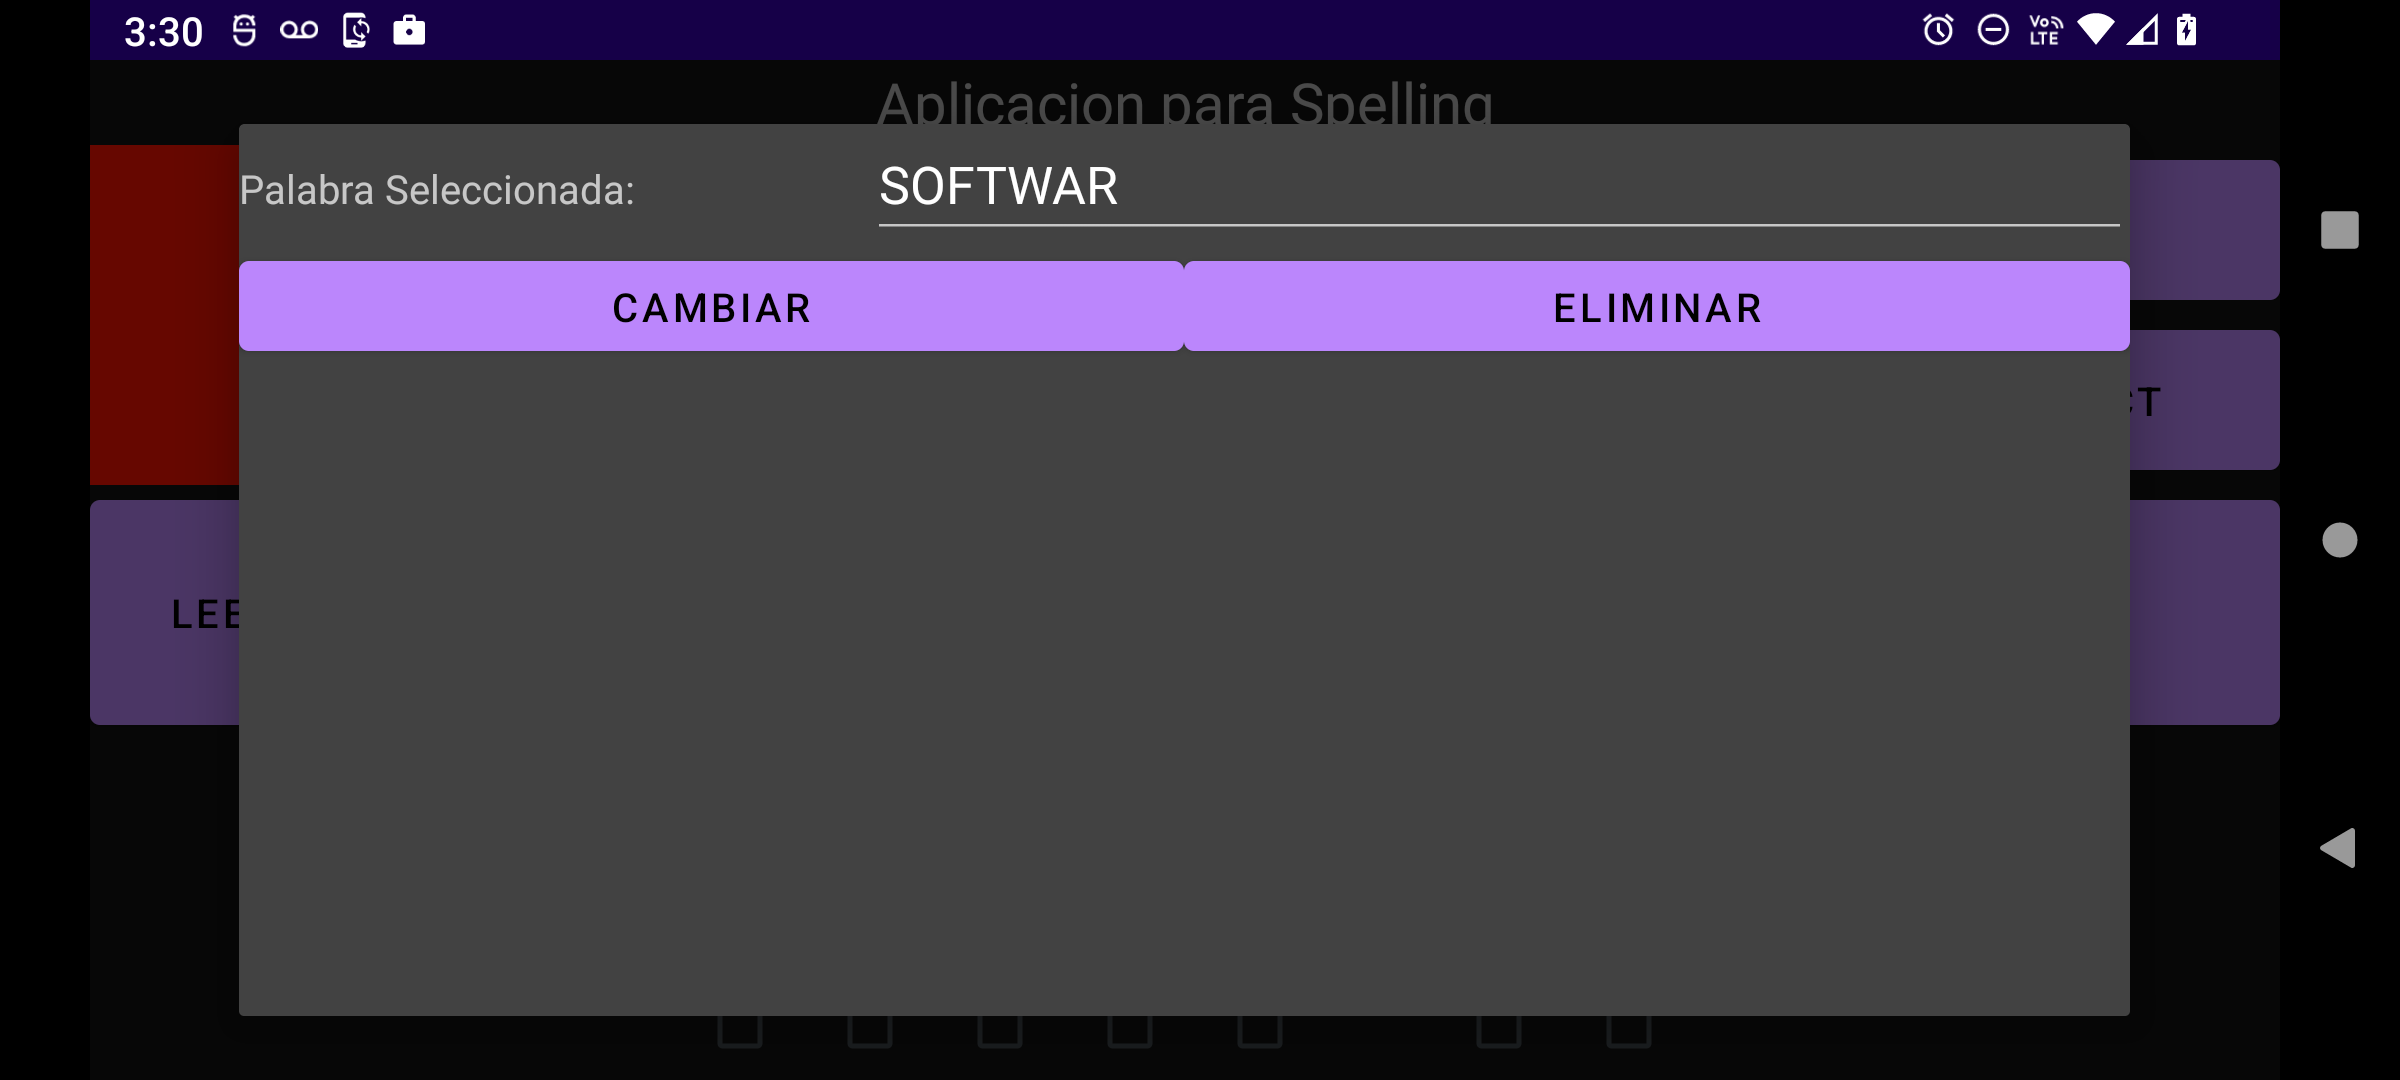
\includegraphics[width=0.46\linewidth]{2022_Spelling/figs/Spelling3.png} \\
	\end{tabular}
\end{center}
\end{frame}

 % Pase lista

\section[JM3D]{Juegos y Modelado 3D}

% Plano Cartesiano y Cubo

\renewcommand{\EntradaBibtex}{Ajedrez3D_2017}
%\setcounter{footnote}{0}


\begin{frame}{\citetitle{\EntradaBibtex} \footnotemark[1] (1)}
%\begin{block}{Multiplayer Chess \footnotemark} 
\begin{columns}
\begin{column}{0.4\textwidth}
		\begin{itemize}
		\item Cada pieza fue modelada en Blender y exportada a la aplicación de Android
		\item Aplicación multidispositivo, que permite llevar una partida de ajedrez.
		\item El control del juego queda del lado del servidor. 
		\end{itemize}

\end{column}
\begin{column}{0.3\textwidth}
%   some text here some text here some text here some text here some text here
     \begin{center}
     %%%%% this is a minipage, so \textwidth is already adjusted to the size of the column
     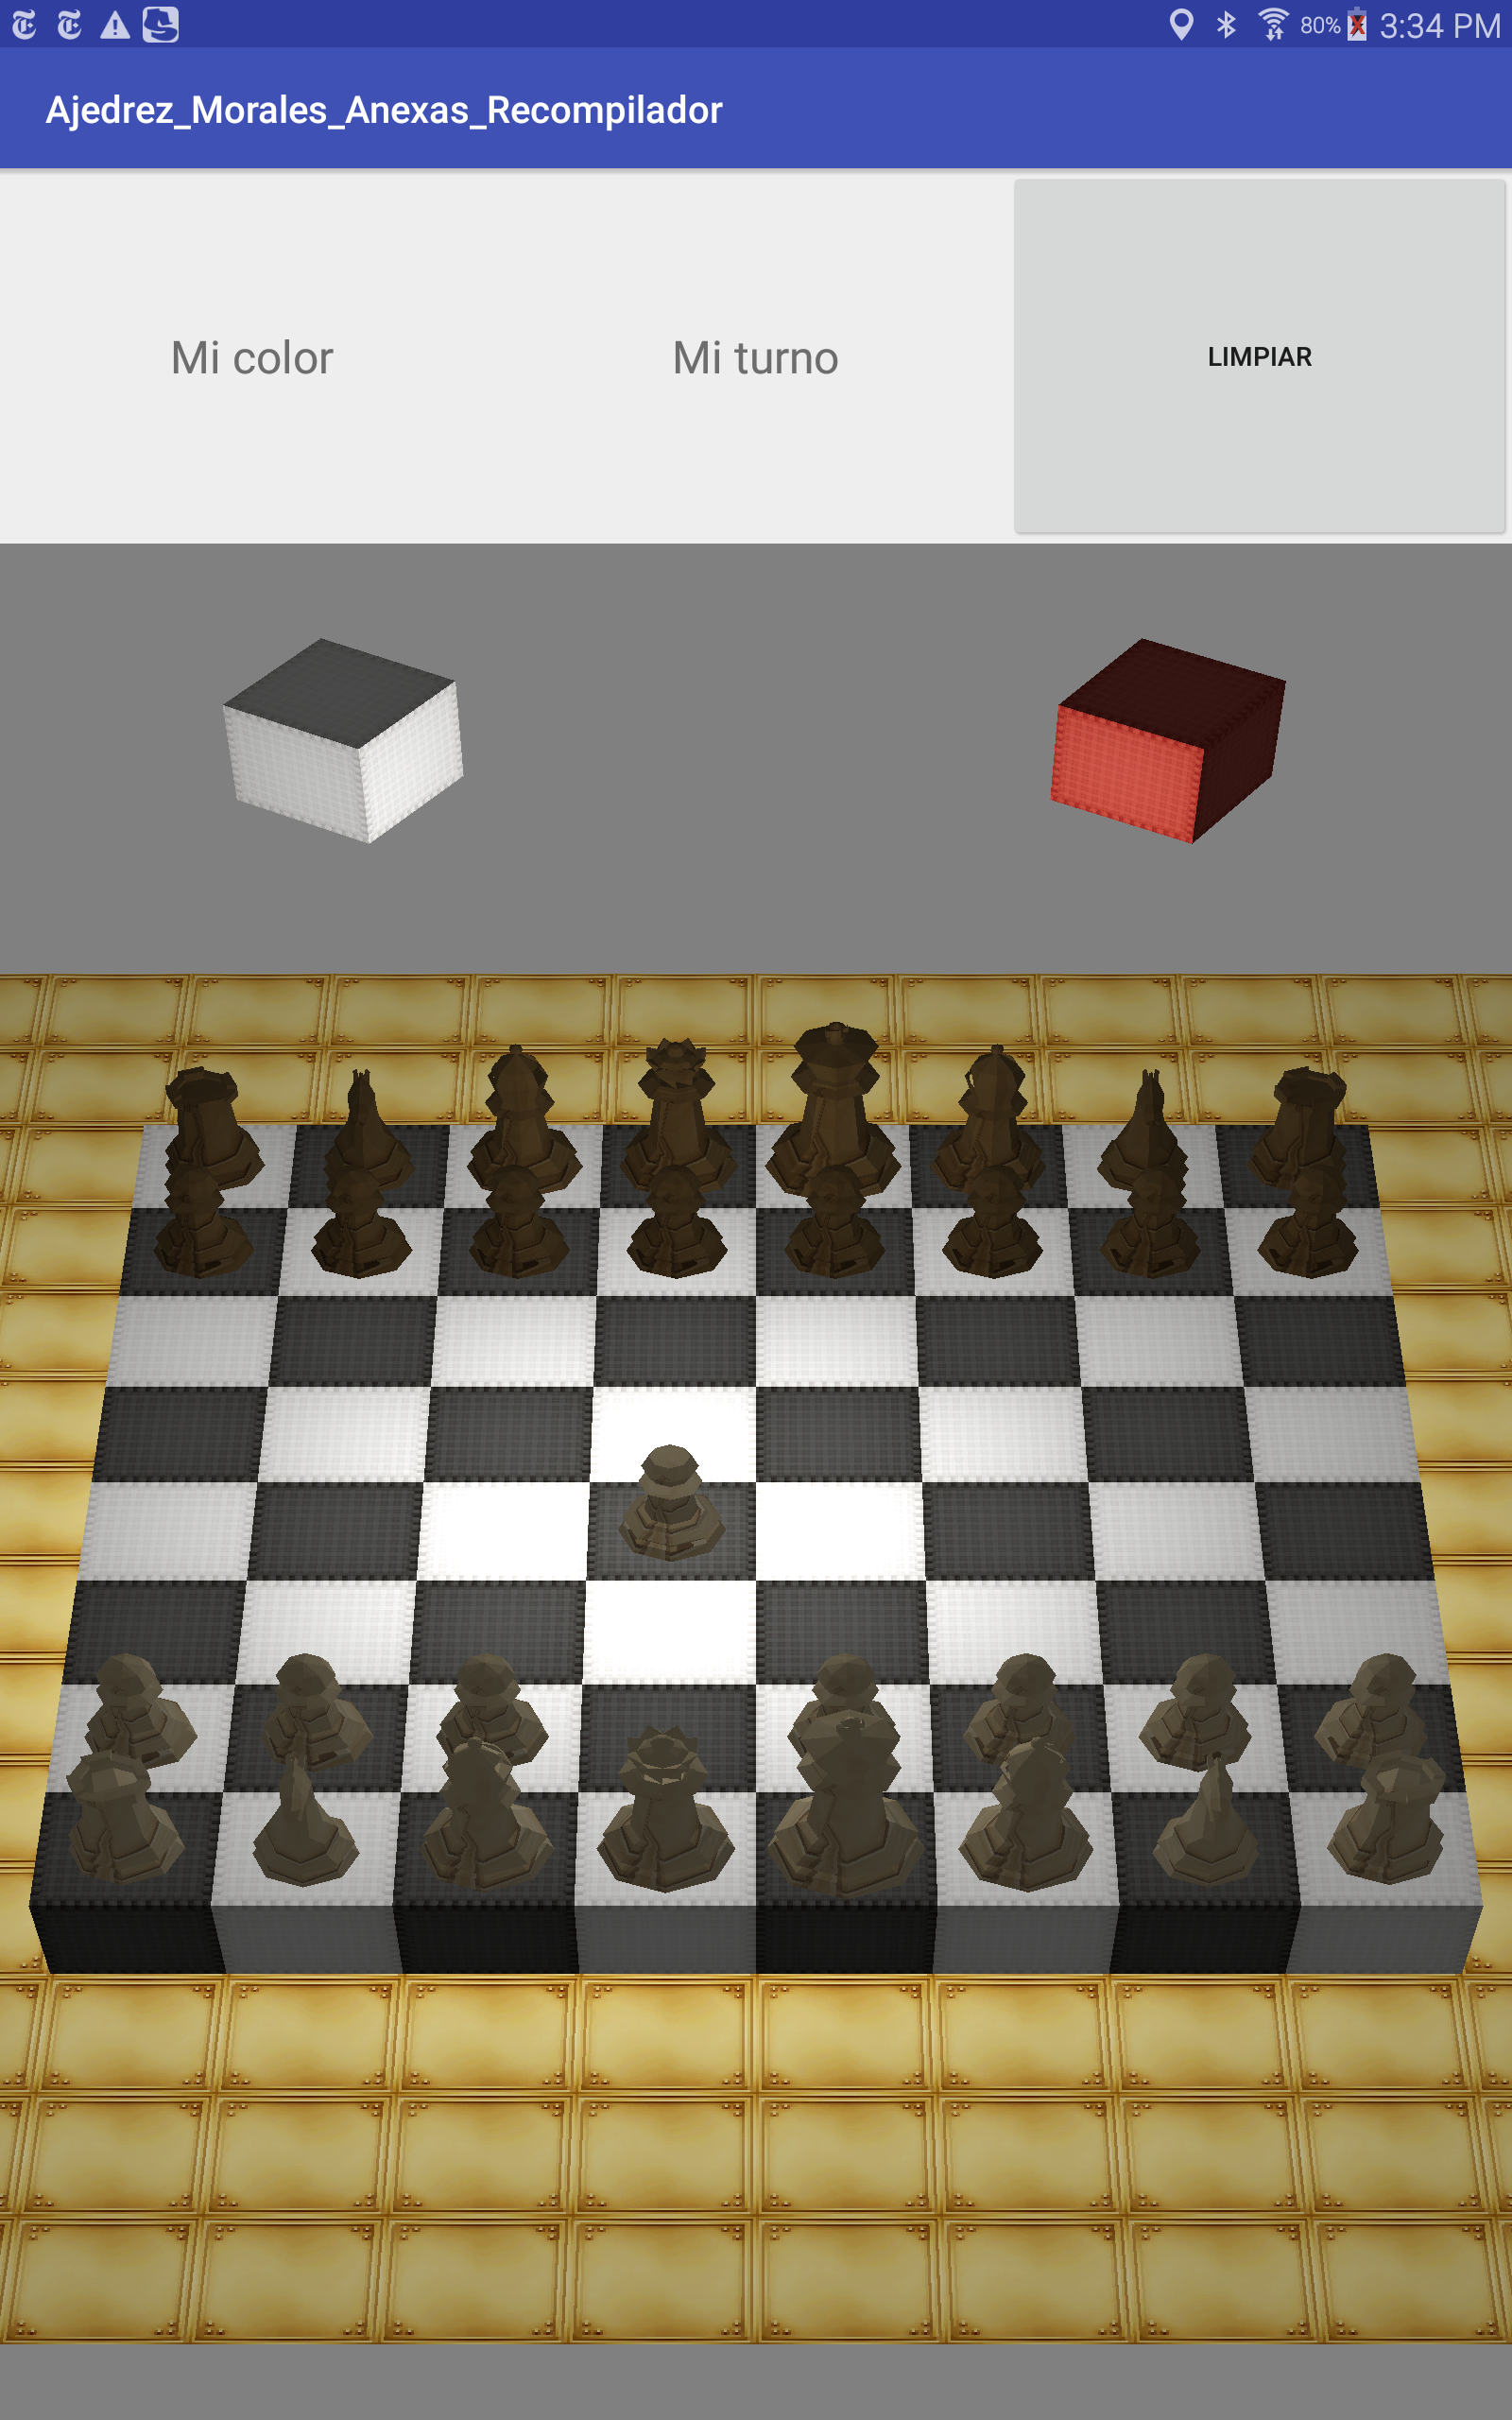
\includegraphics[width=0.7\textwidth]{Figs/Ajedrez_01}
     \end{center}

\end{column}
\begin{column}{0.3\textwidth}  
    \begin{center}
     %%%%% this is a minipage, so \textwidth is already adjusted to the size of the column
     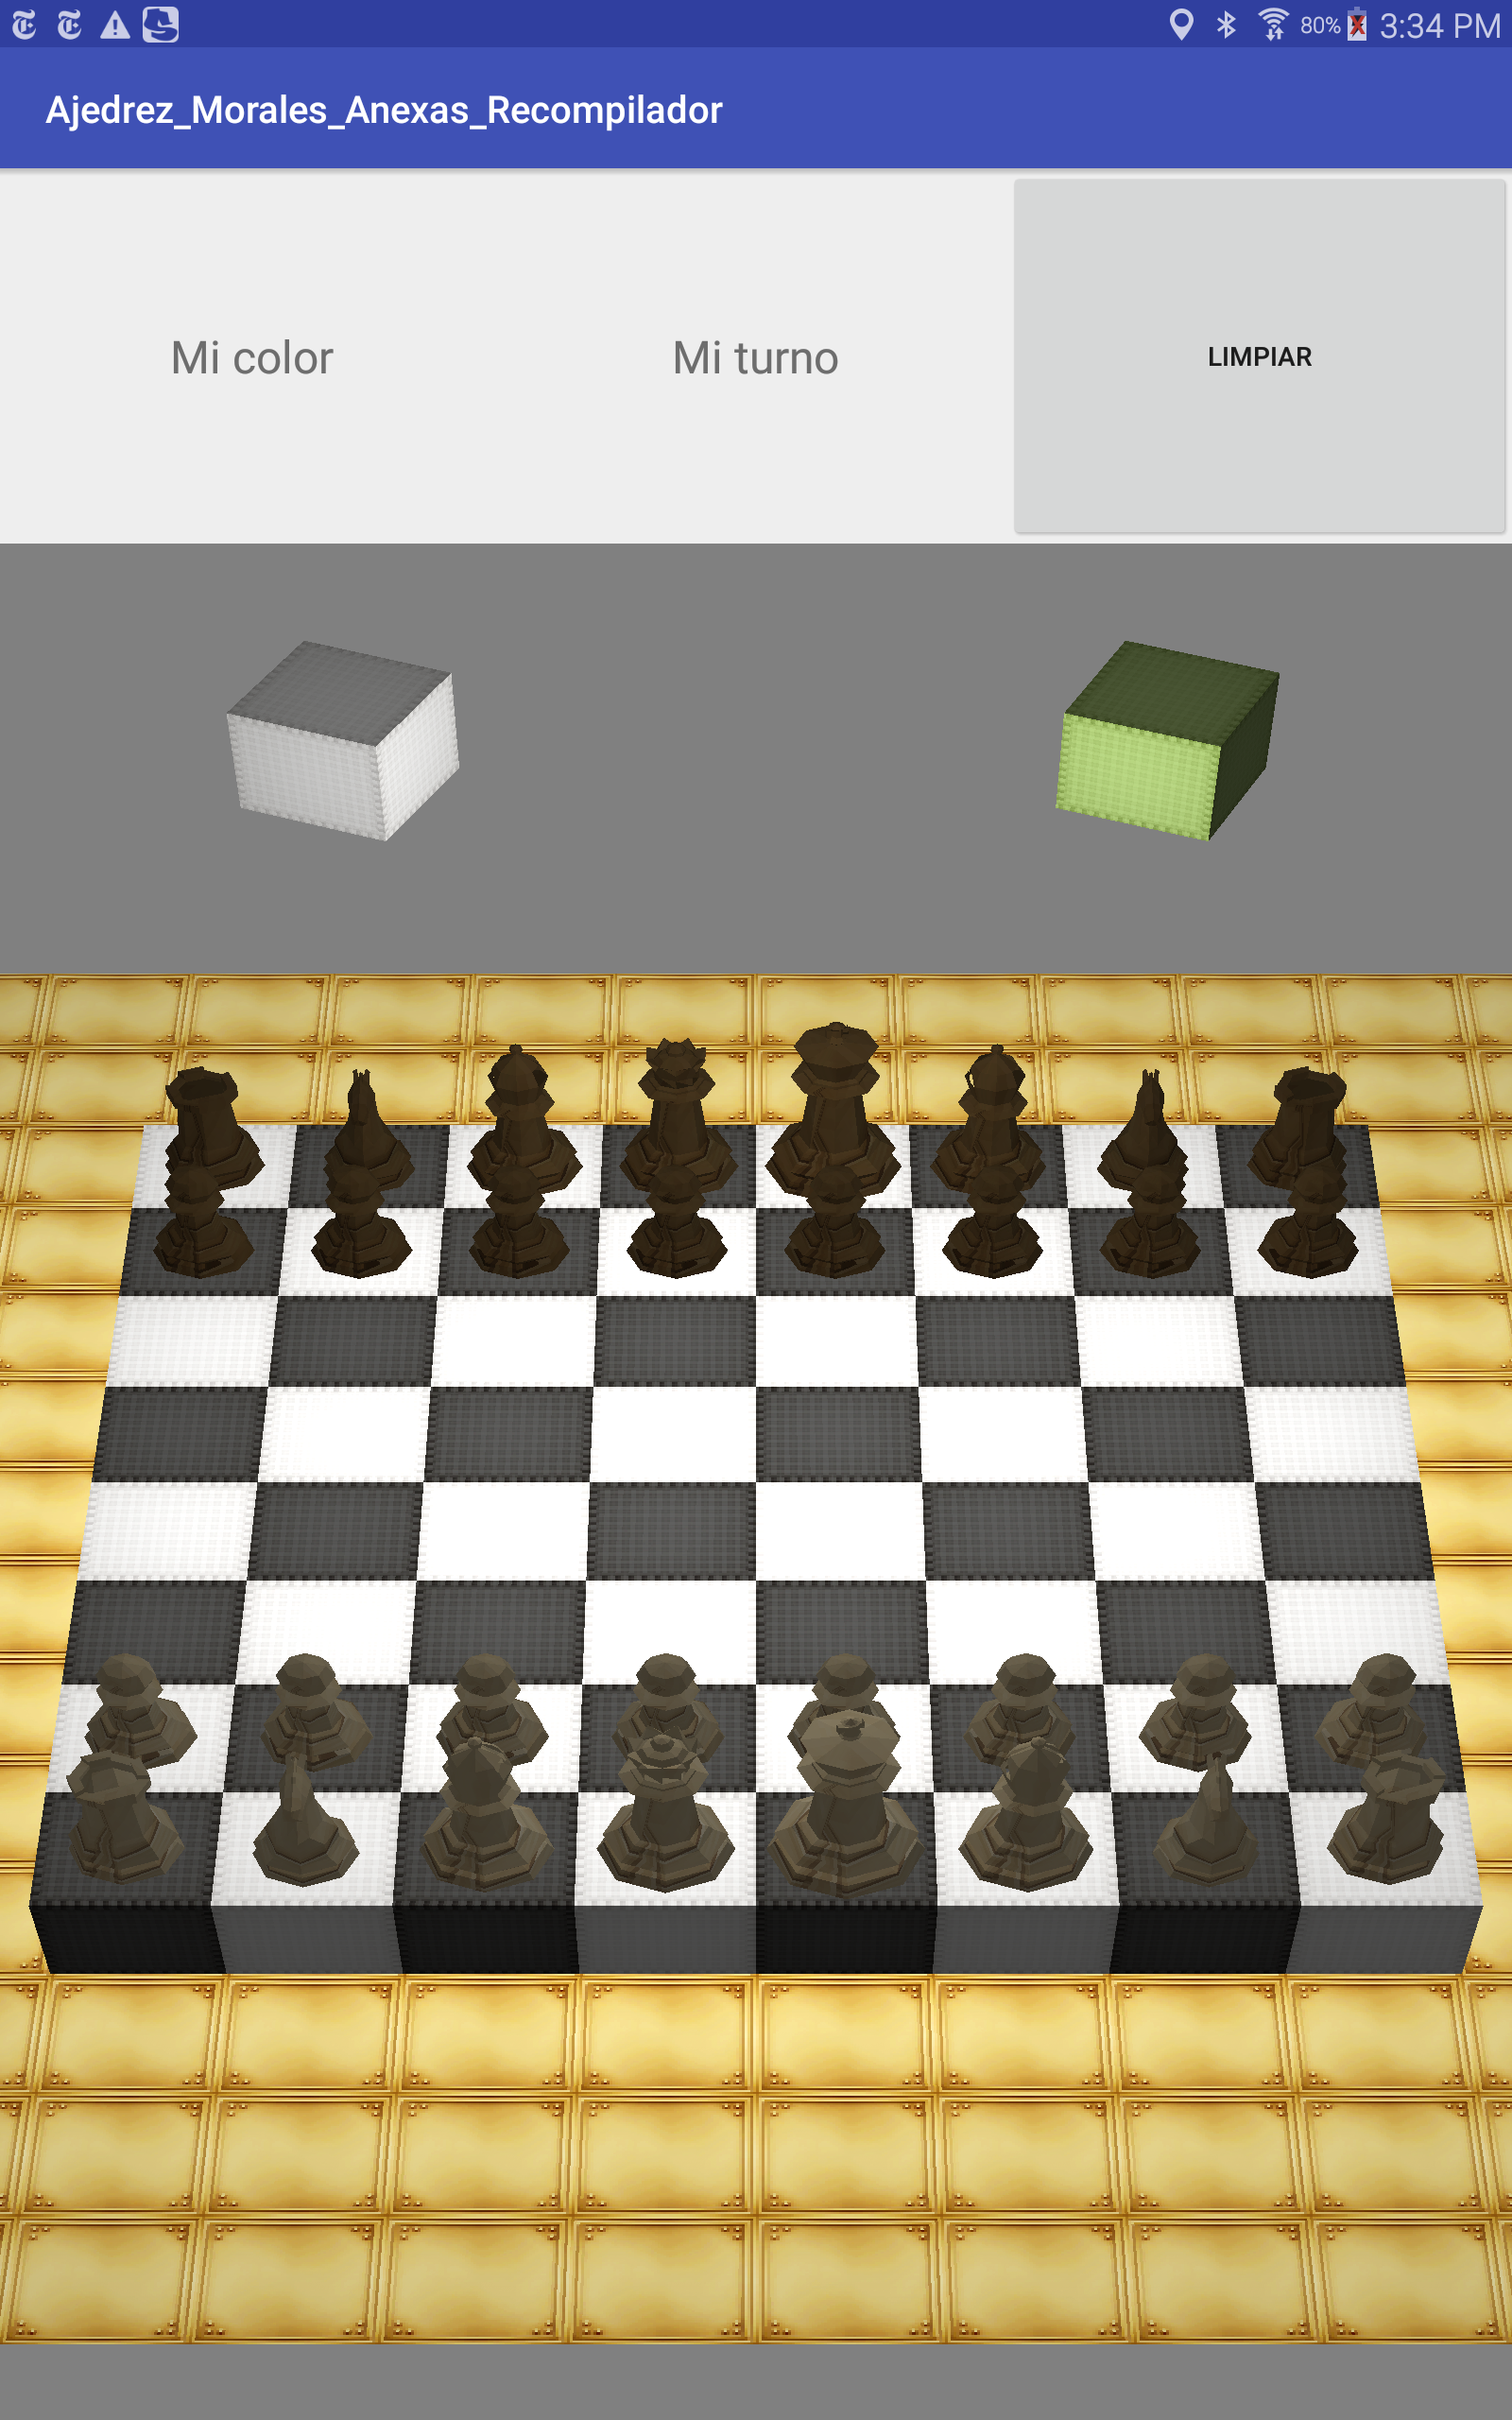
\includegraphics[width=0.7\textwidth]{Figs/Ajedrez_02}
     \end{center}
\end{column}
\end{columns}
%\footfullcite*{\EntradaBibtex}
\footnotetext[1]{\fullcite{\EntradaBibtex}}
\end{frame}



\renewcommand{\EntradaBibtex}{CruzdeMalta_2017}

\begin{frame}{\citetitle{\EntradaBibtex} \footnotemark[1] (1)}
%\begin{block}{Simulación del Mecanismo de la Cruz de Malta\footnotemark} 
	\begin{itemize}
	\item Se modelaron los componentes individuales 3D (cilindros, tetaedros, etc)
	\item Se incorporó texturas, iluminación y sombras
	\item Es posible ver el modelo desde múltiples perspectivas
	\end{itemize}
\begin{columns}
	\begin{column}{0.48\textwidth}
    \begin{center}
     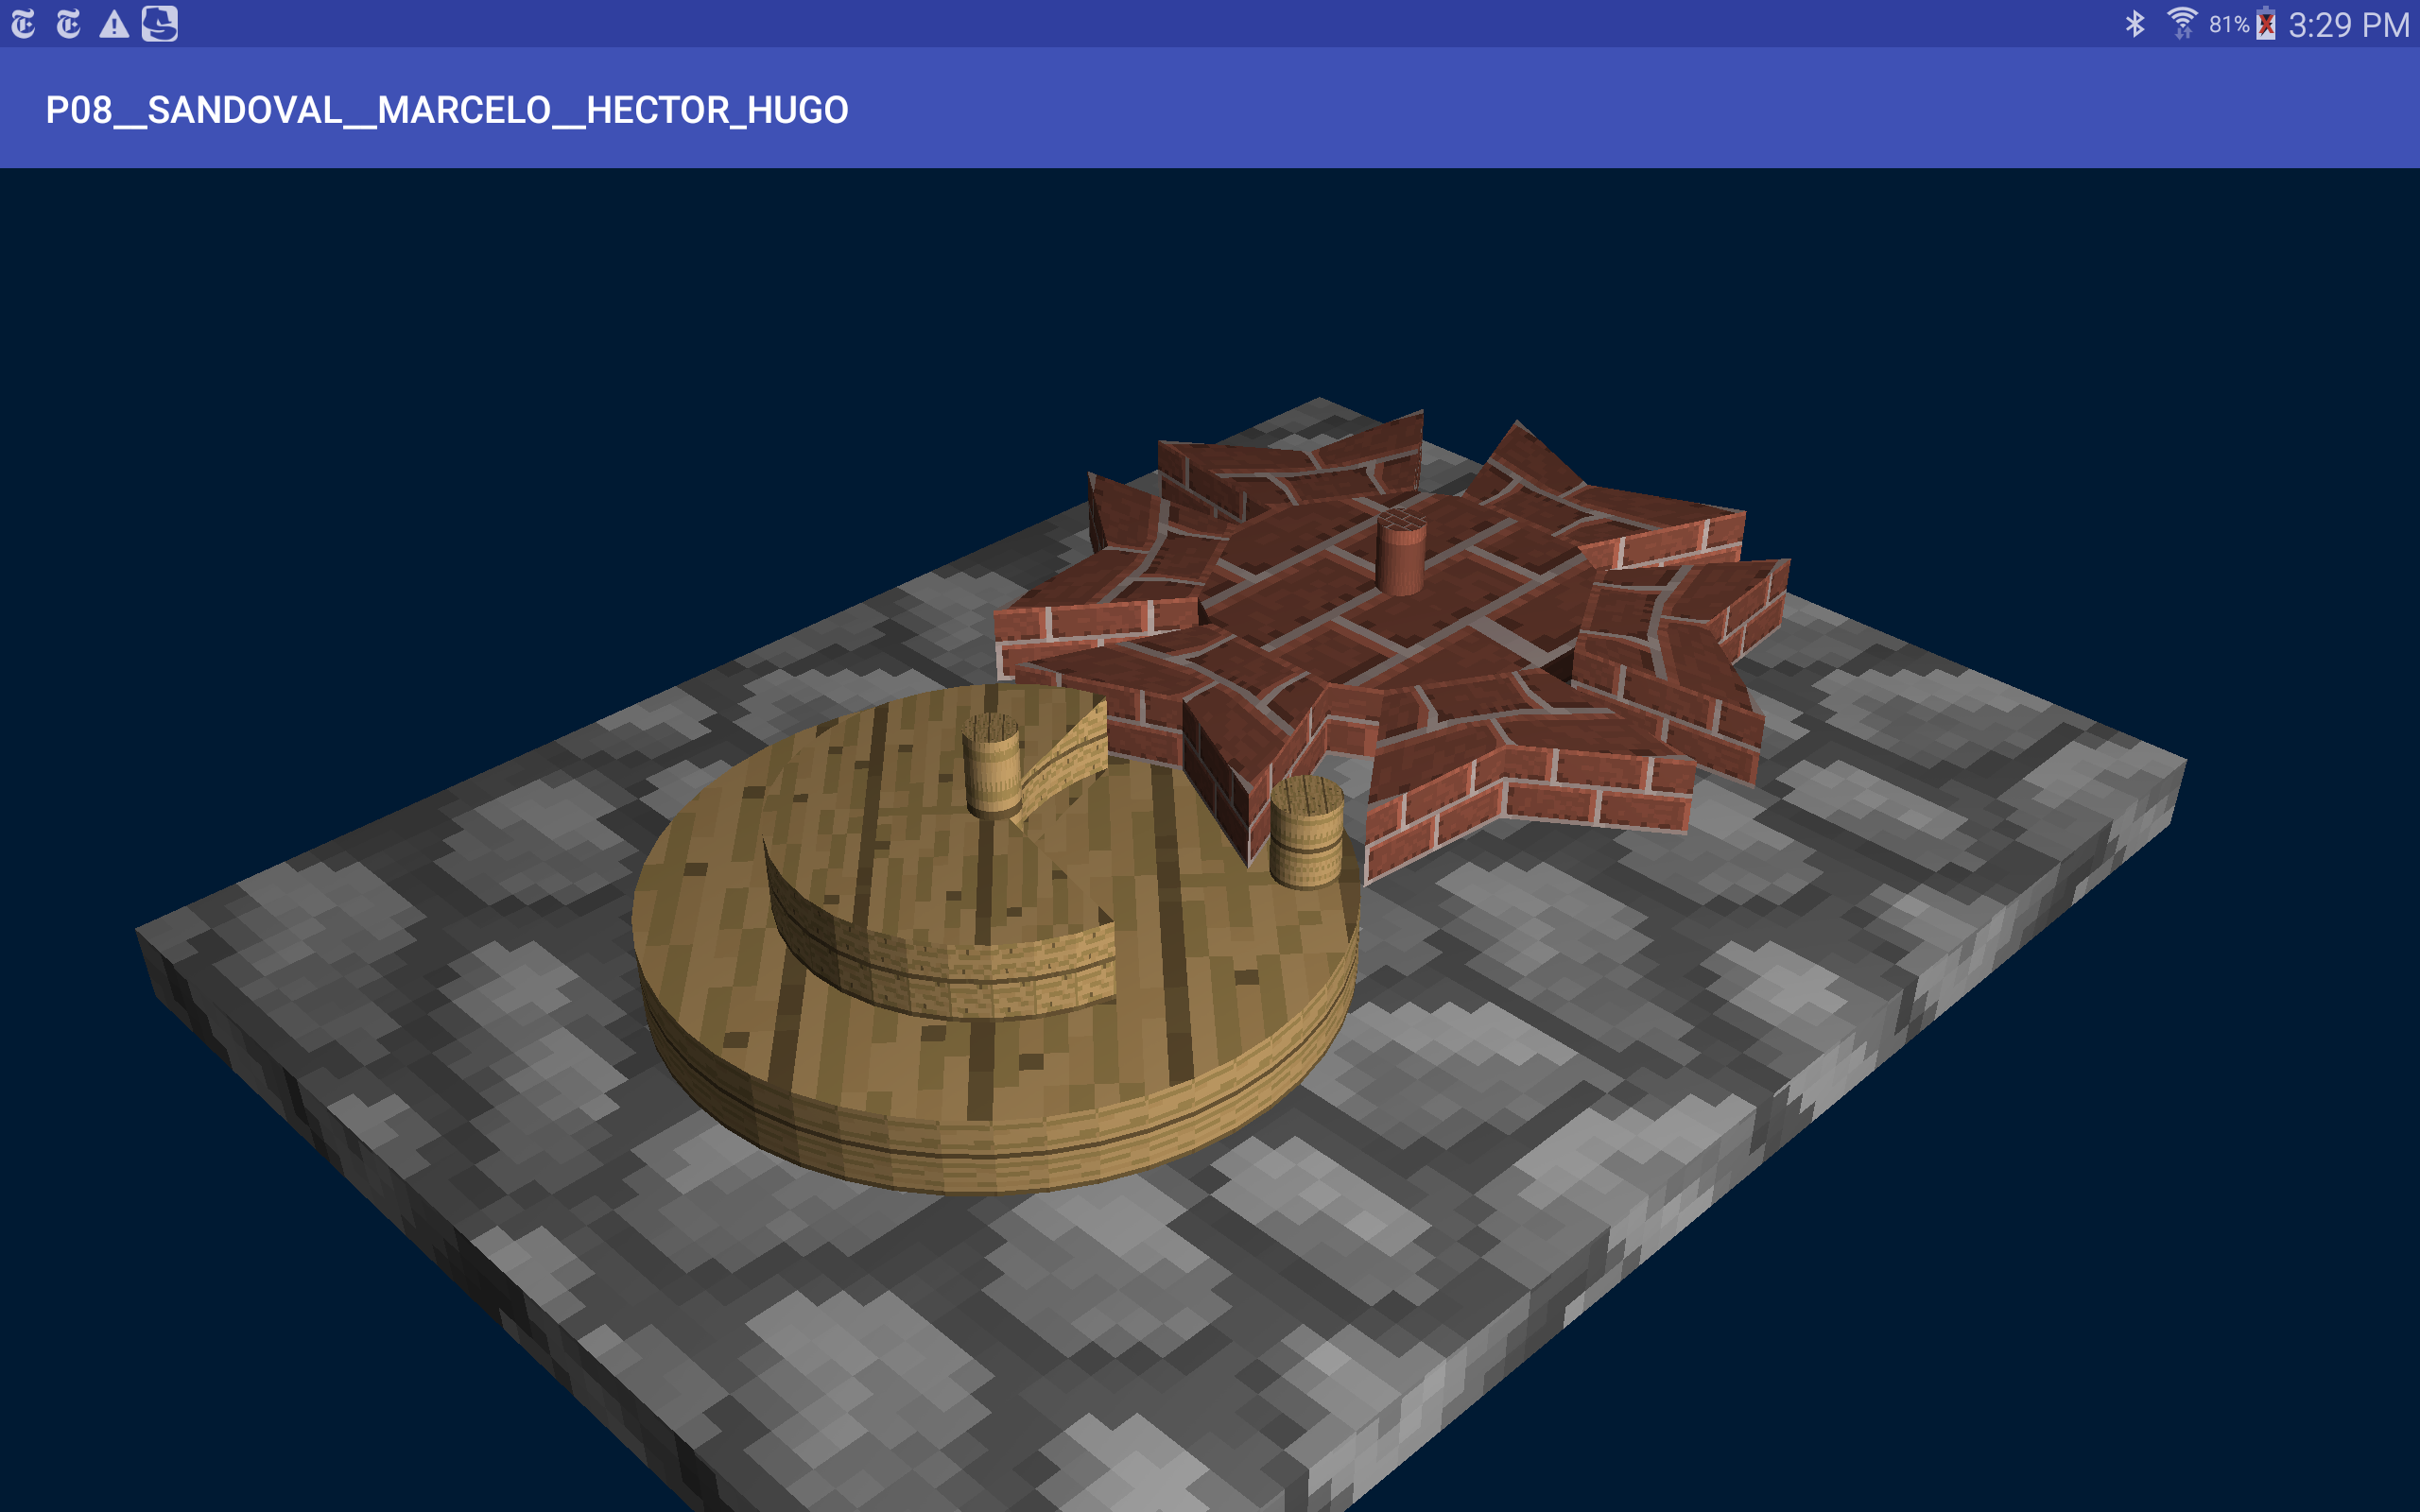
\includegraphics[width=0.7\textwidth]{Figs/CruzMalta_01}
     \end{center}
\end{column}
\begin{column}{0.48\textwidth}  
    \begin{center}
     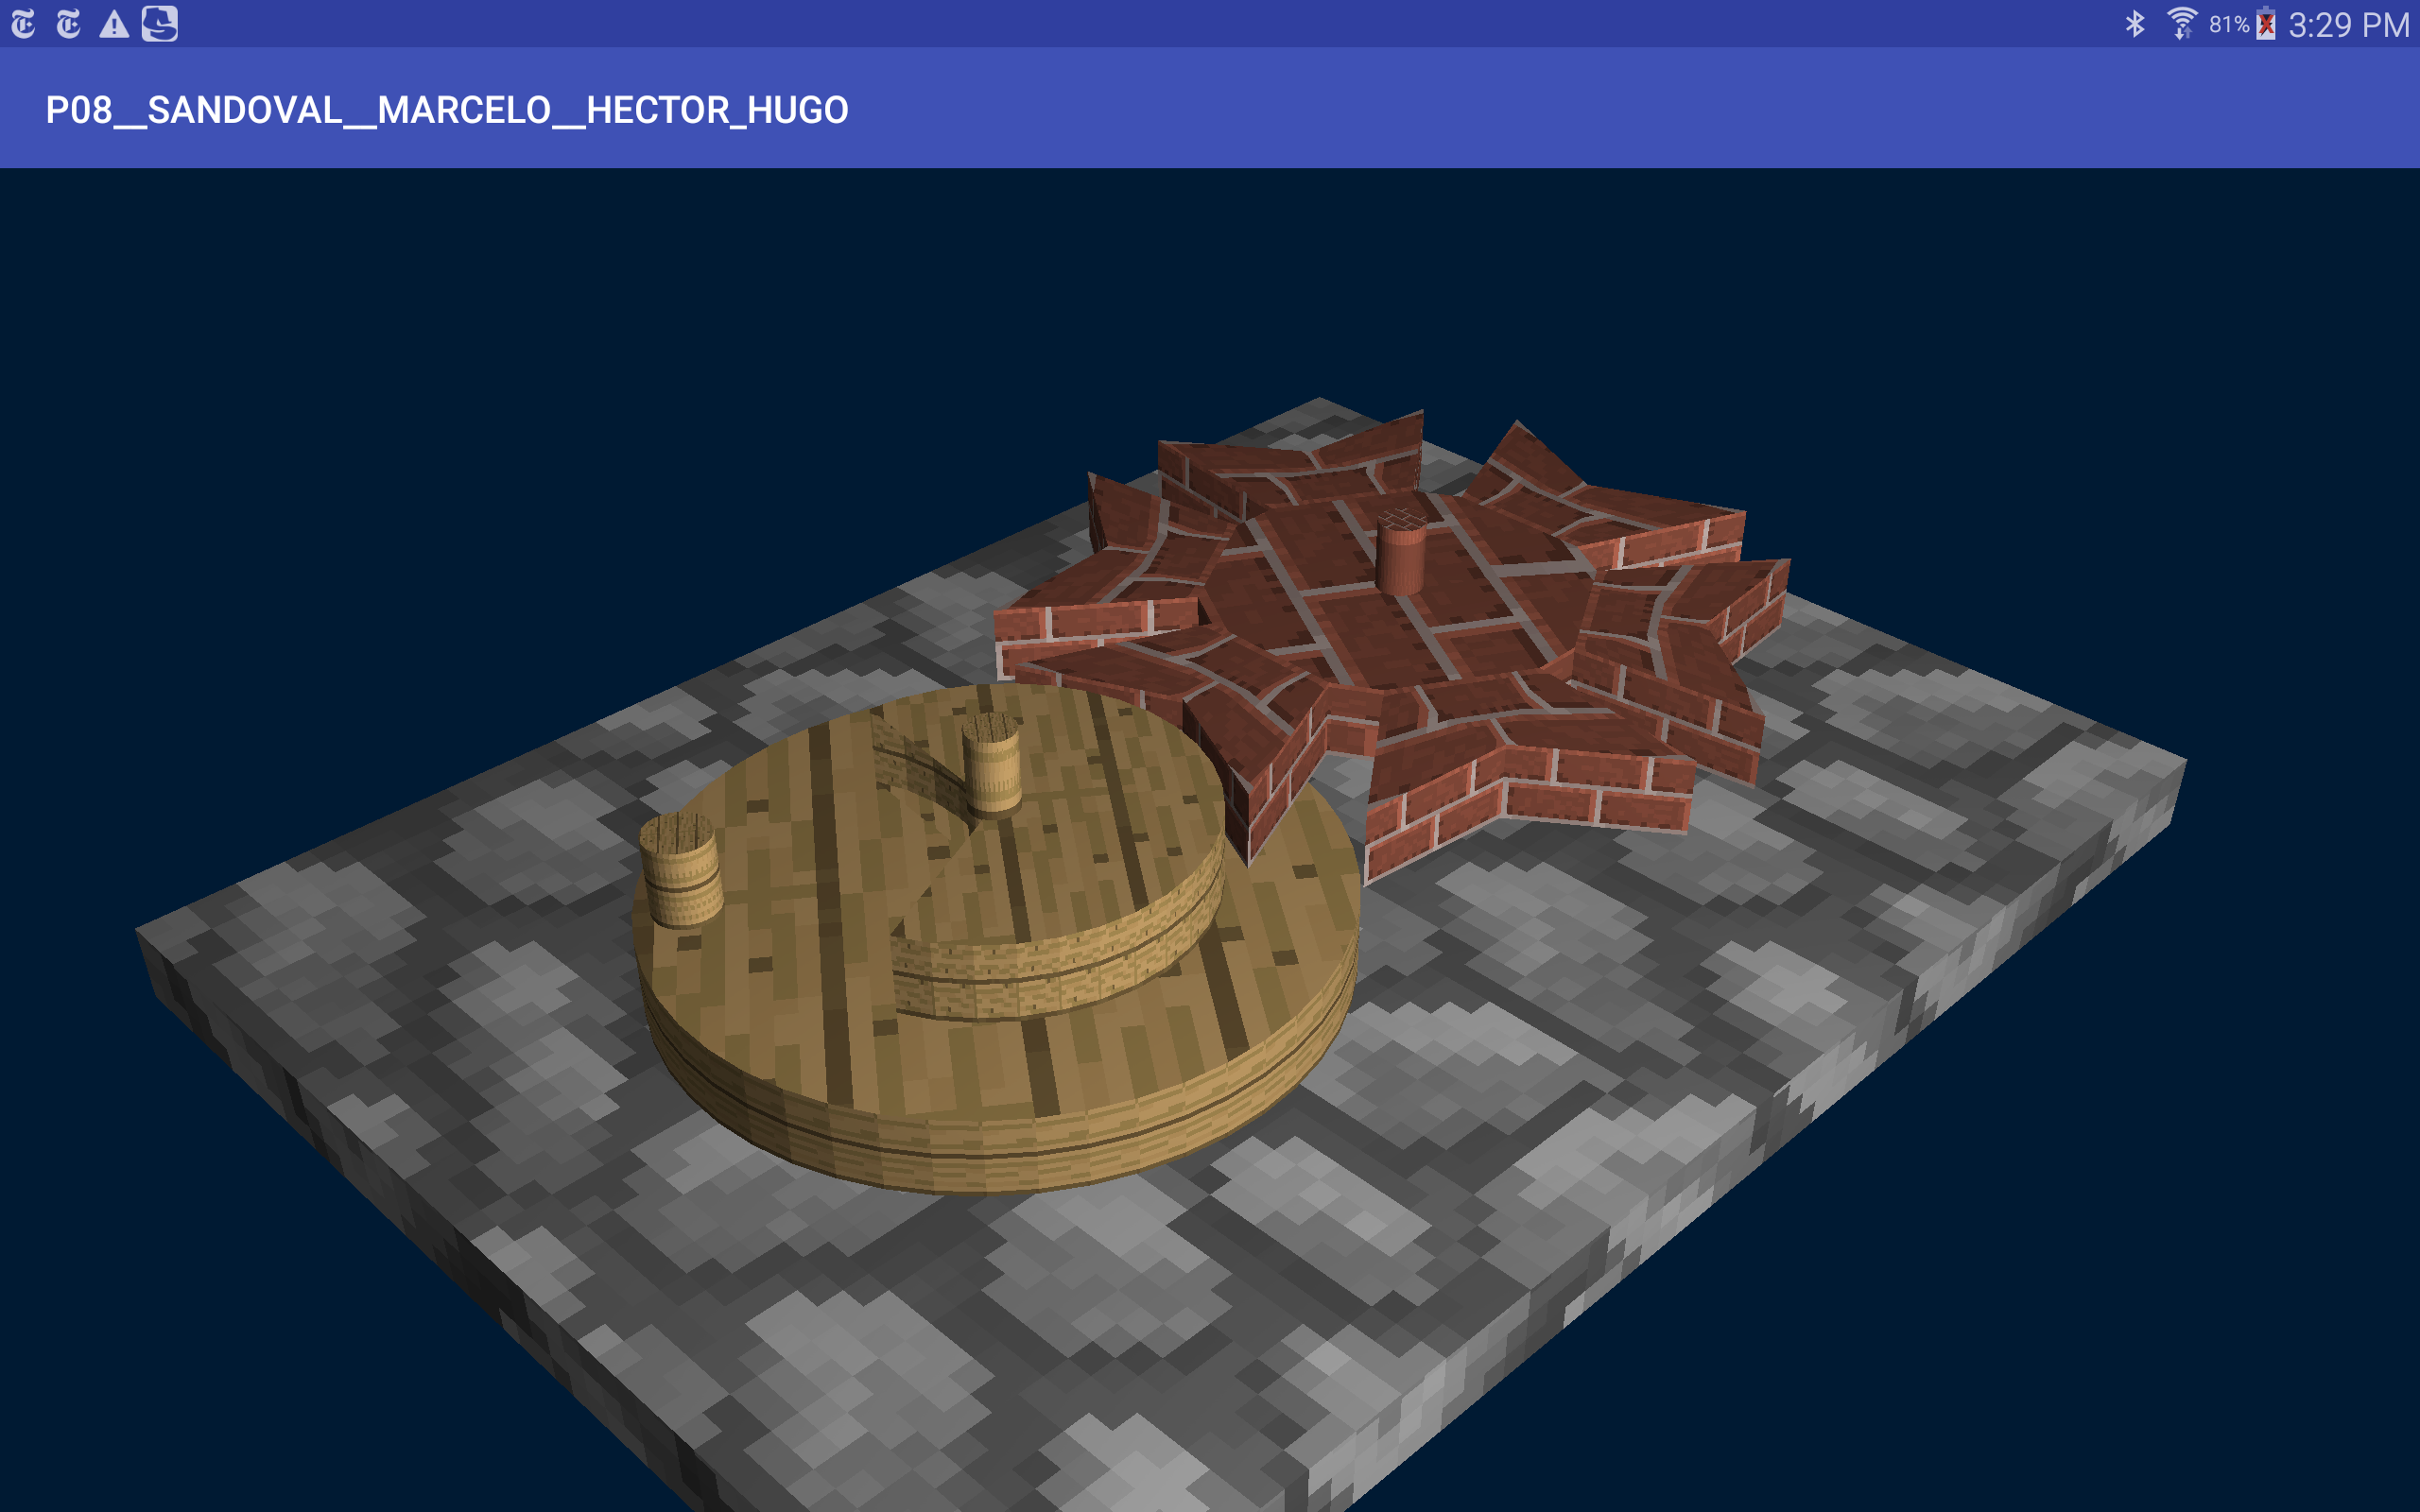
\includegraphics[width=0.7\textwidth]{Figs/CruzMalta_02}
     \end{center}
\end{column}
\end{columns}
%\end{block} 
\footnotetext[1]{\fullcite{\EntradaBibtex}}
%\footnotetext{Héctor Hugo Sandoval Marcelo. \textbf{Movimiento de la Cruz de Malta con Iluminación y Texturas con Java y OpenGL ES 2.0 en Android.}. Universidad Politécnica de Victoria,  Informe técnico proyecto de asignatura ``Graficación por Computadora Avanzada'', 2017. Sin Publicar.}
%\\setcounter{footnote}{0}
\end{frame}




\renewcommand{\EntradaBibtex}{Reporte2017_Tetris3D}

\begin{frame}{\citetitle{\EntradaBibtex} \footnotemark[1] (1)}
\begin{block}{Motivación} 
Este proyecto esta inspirado en un tetris 3D para PC \url{http://users.csc.calpoly.edu/~zwood/teaching/csc471/finalproj24/gzipkin/}
\begin{itemize}
\item Varias piezas caen sobre una rejilla y el objetivo es borar las lineas.
\item Las piezas se mueven en un entorno tridimensional (ejes X, Y y Z)
\item Las fronteras de la red estan definidas mediante una malla alámbrica
\item La cámara tambien se puede mover en base a eventos de toque sobre la pantalla del dispositivo
\end{itemize}
\end{block} 
\footnotetext[1]{\fullcite{\EntradaBibtex}}
\end{frame}


\begin{frame}{Aplicación Tetris 3D (2)}
%\begin{block}{Pantallas Principales} 
\begin{center}
	\begin{tabular}{cccc}
		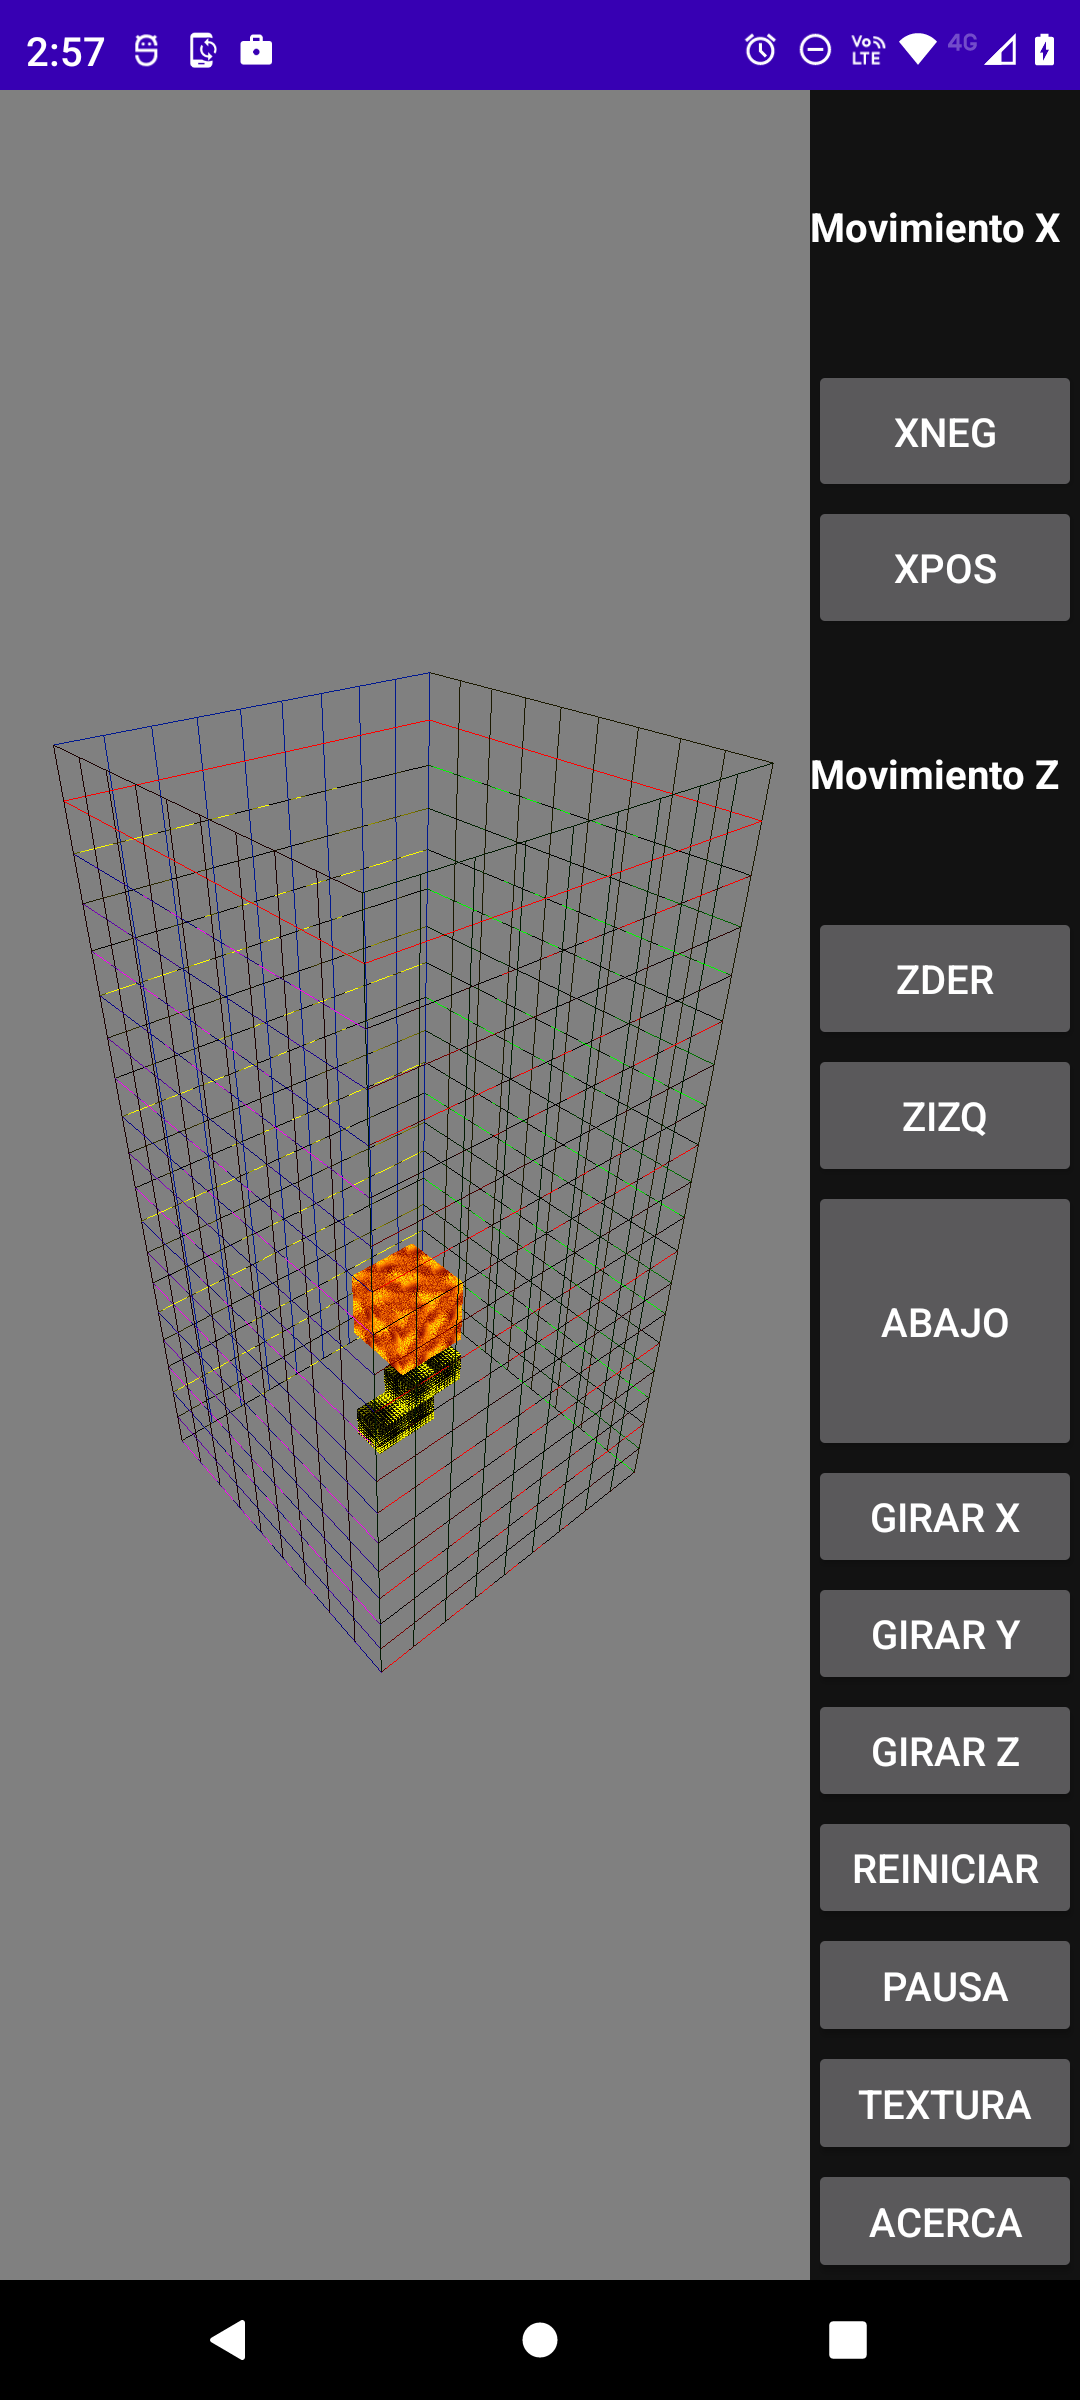
\includegraphics[width=0.20\linewidth]{2017_Tetris3D/figs/Tetris0.png} &
		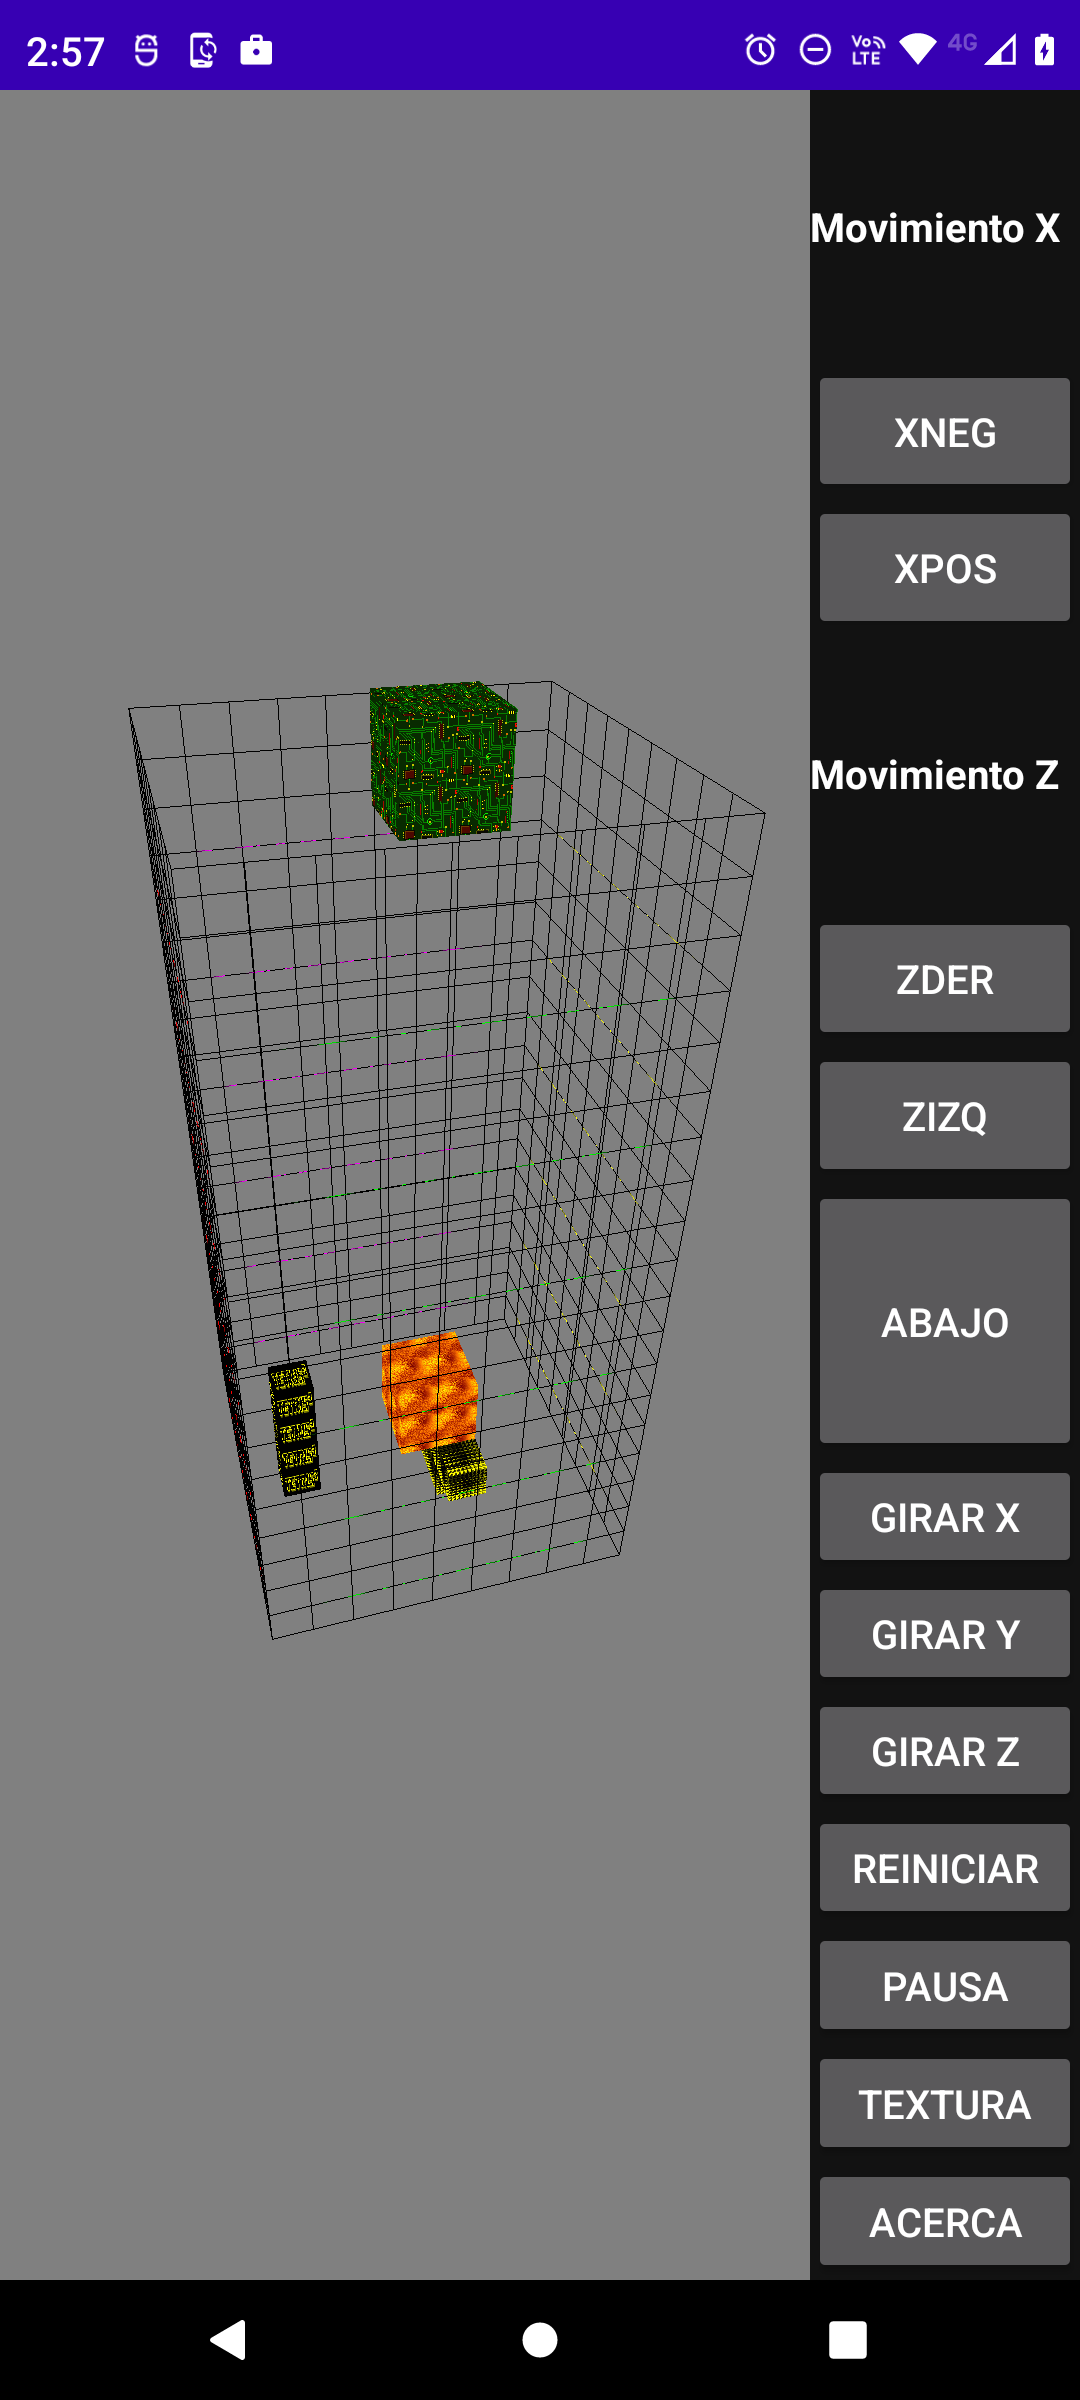
\includegraphics[width=0.20\linewidth]{2017_Tetris3D/figs/Tetris1.png} & 		 		
		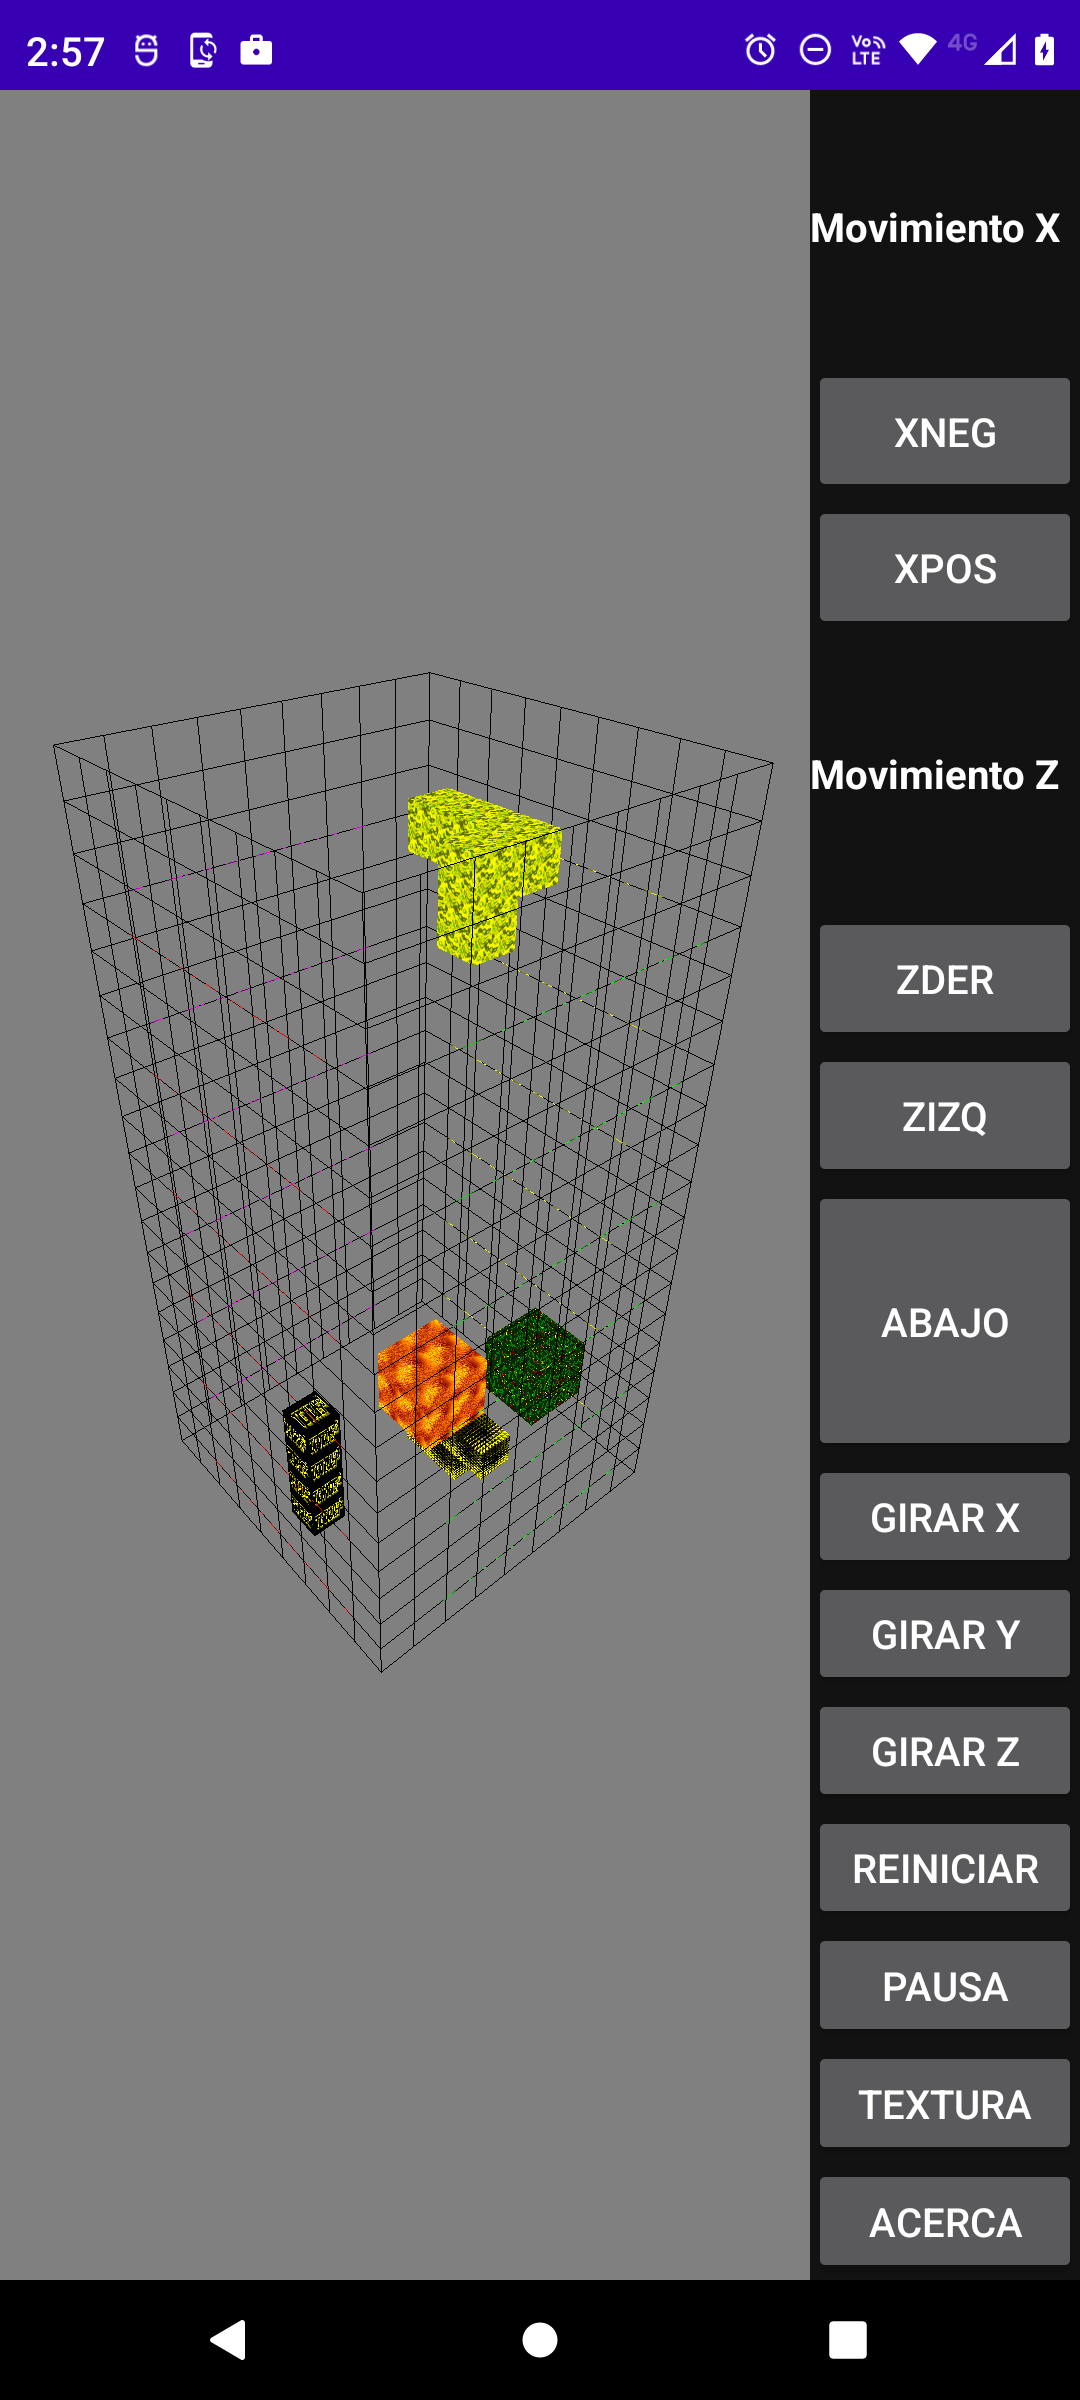
\includegraphics[width=0.20\linewidth]{2017_Tetris3D/figs/Tetris2.png} & 		
		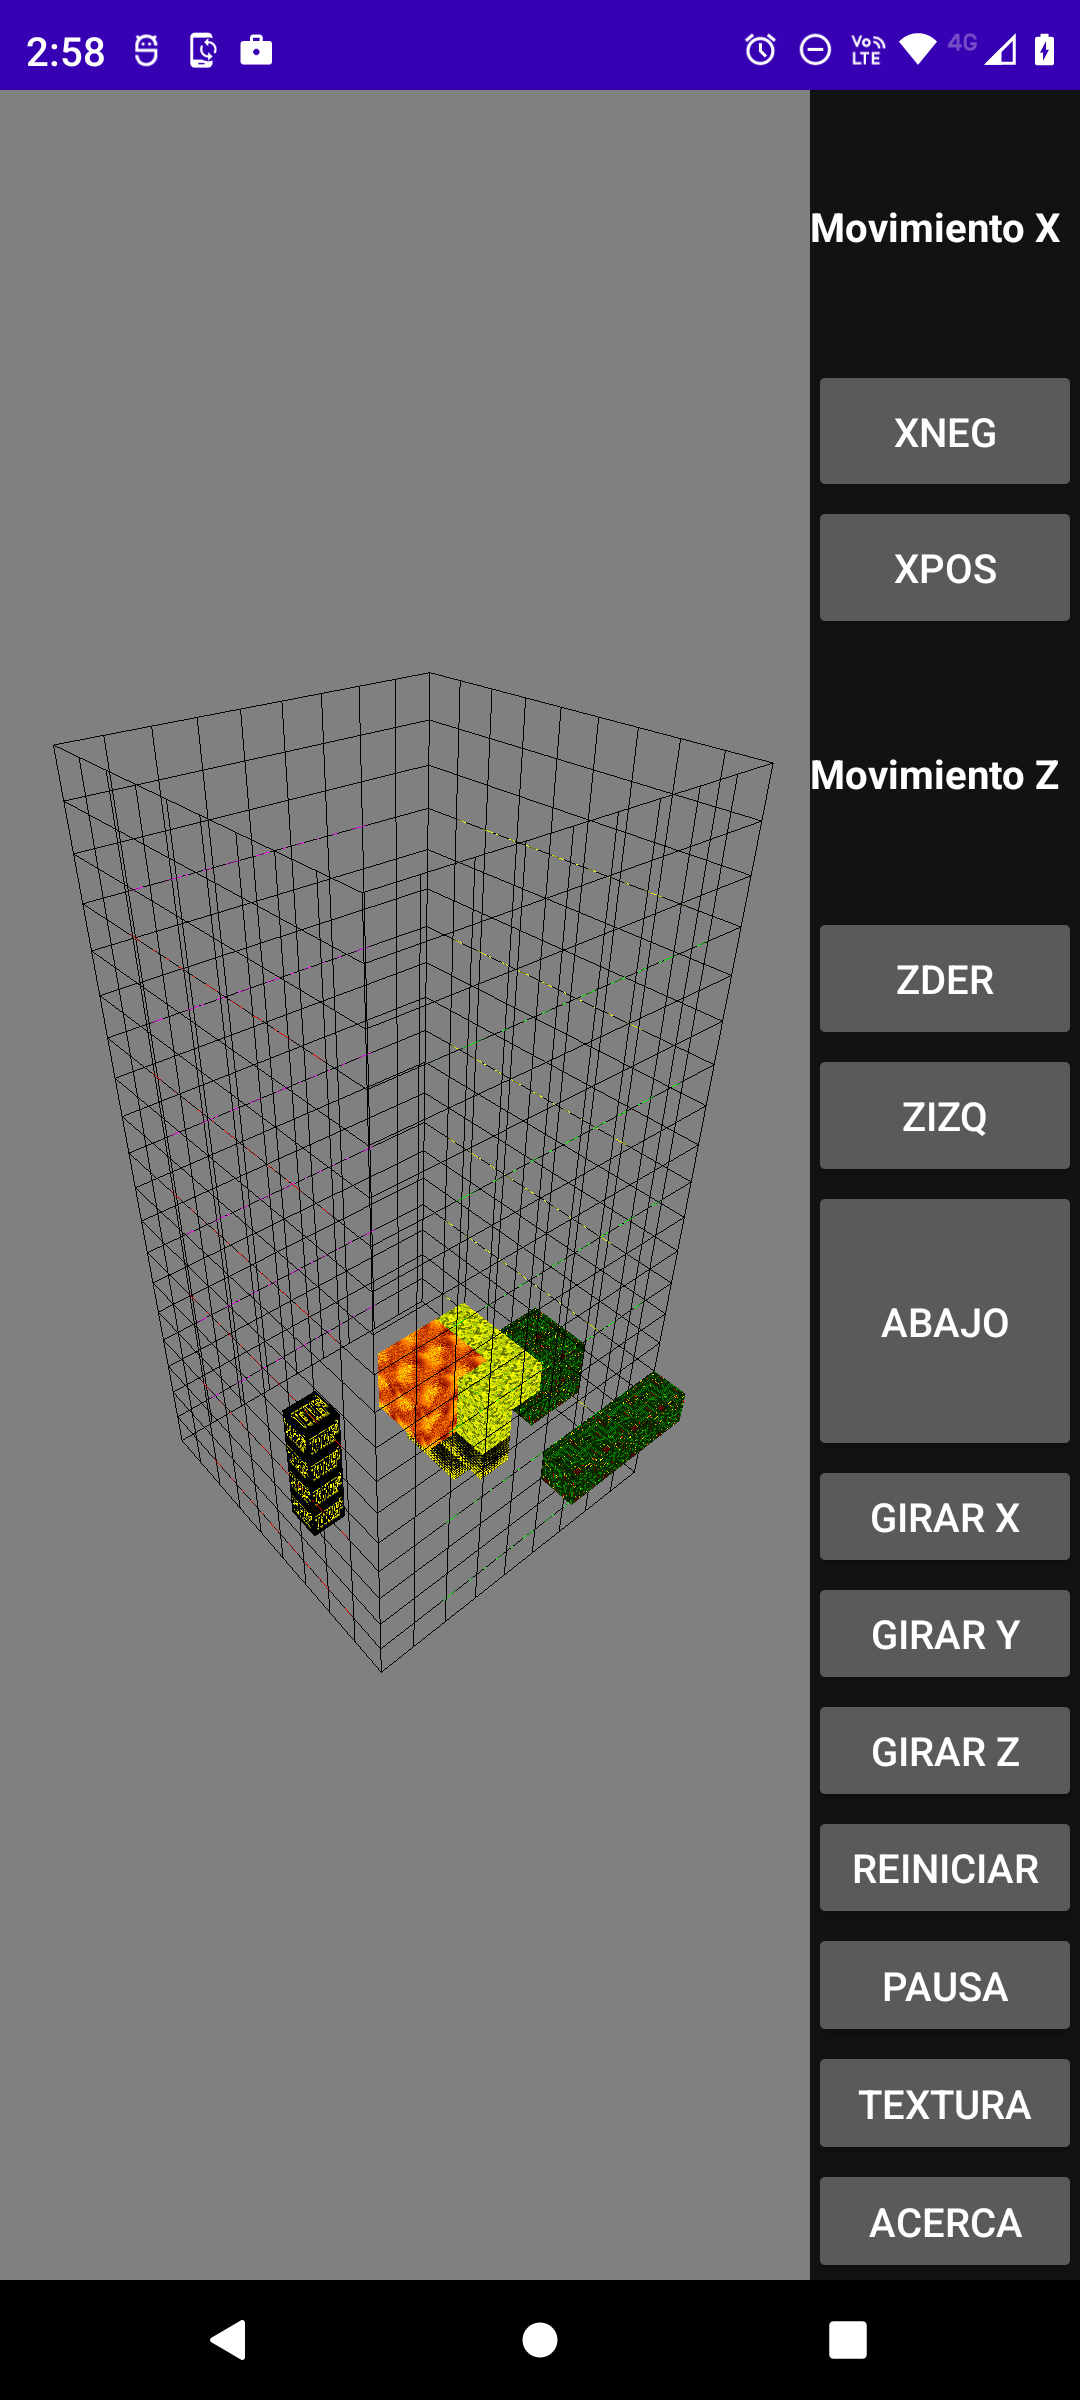
\includegraphics[width=0.20\linewidth]{2017_Tetris3D/figs/Tetris3.png} \\
	\end{tabular}
\end{center}
\end{frame}



 % Tetris 3D

\renewcommand{\EntradaBibtex}{BrazoRobot_Morin2019}
\begin{frame}{\citetitle{\EntradaBibtex} \footnotemark[1] (1)}
%\begin{block}{Brazo Robótico \footnotemark} 
\begin{columns}
	\begin{column}{0.55\textwidth}
		\begin{itemize}
			\item Se retoma un diseño previamente realizado para WebGL. 
			\item Los componentes del robot son movidos mediante motores, y puede ser visto desde difentes perspectivas.		
		\end{itemize}
	\end{column}
	\begin{column}{0.22\textwidth}
		 \begin{center}
		     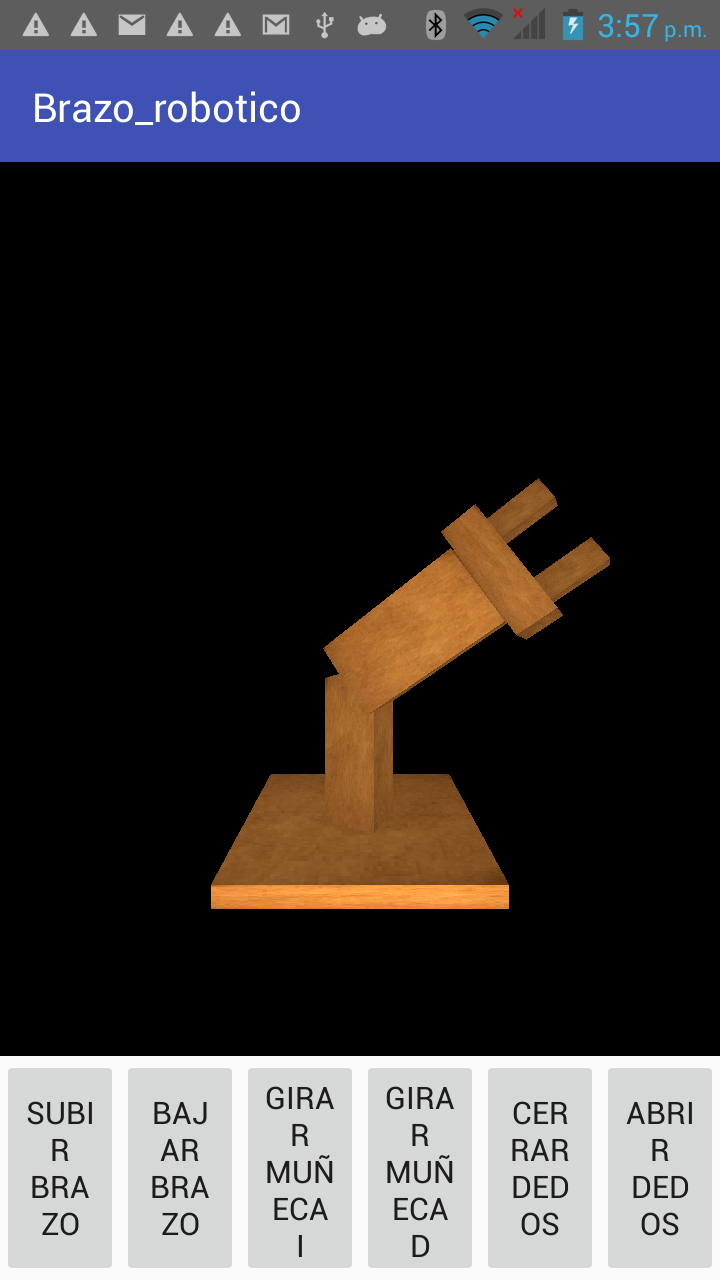
\includegraphics[width=0.98\textwidth]{Figs/brazoRobotico1}
		 \end{center}
	\end{column}
	\begin{column}{0.22\textwidth}  
		\begin{center}
		 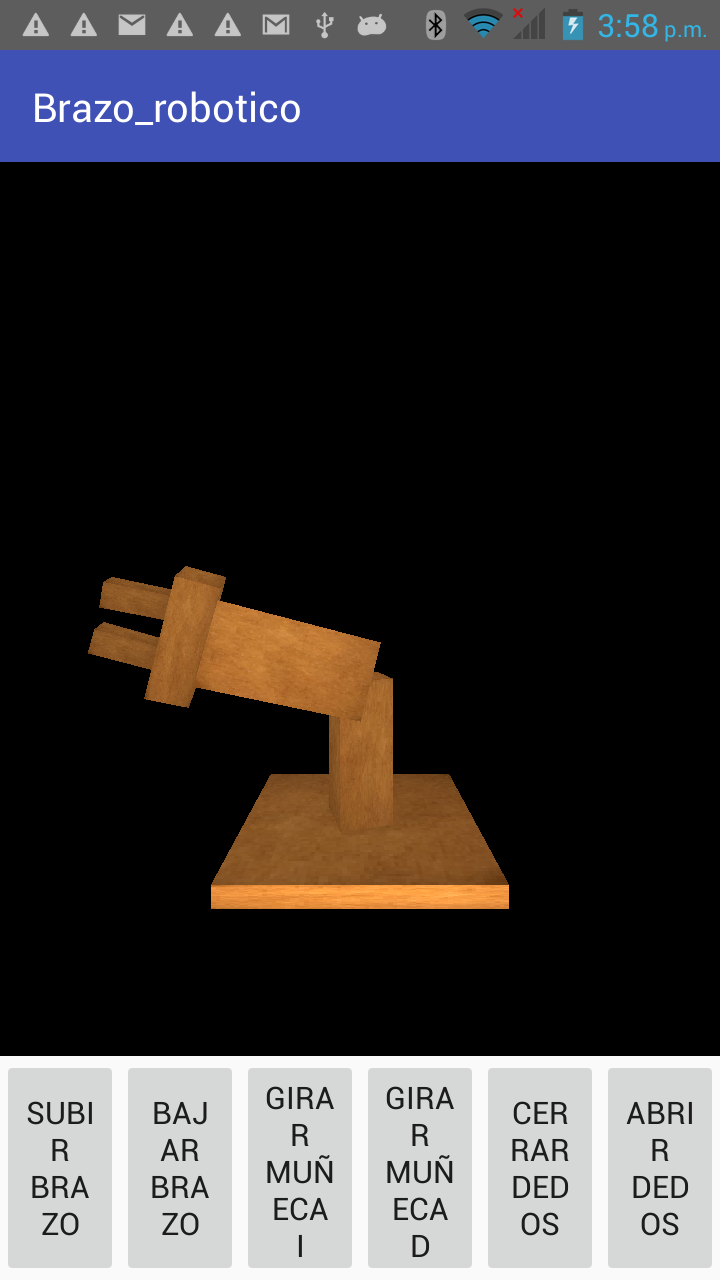
\includegraphics[width=0.98\textwidth]{Figs/brazoRobotico2}
		 \end{center}
	\end{column}
\end{columns}
%\end{block} 
\footnotetext[1]{\fullcite{\EntradaBibtex}}
\end{frame}

\renewcommand{\EntradaBibtex}{BrazoRobot_Uriegas2022}

\begin{frame}{\citetitle{\EntradaBibtex} \footnotemark[1] (1)}
\begin{columns}
\begin{column}{0.25\textwidth}  
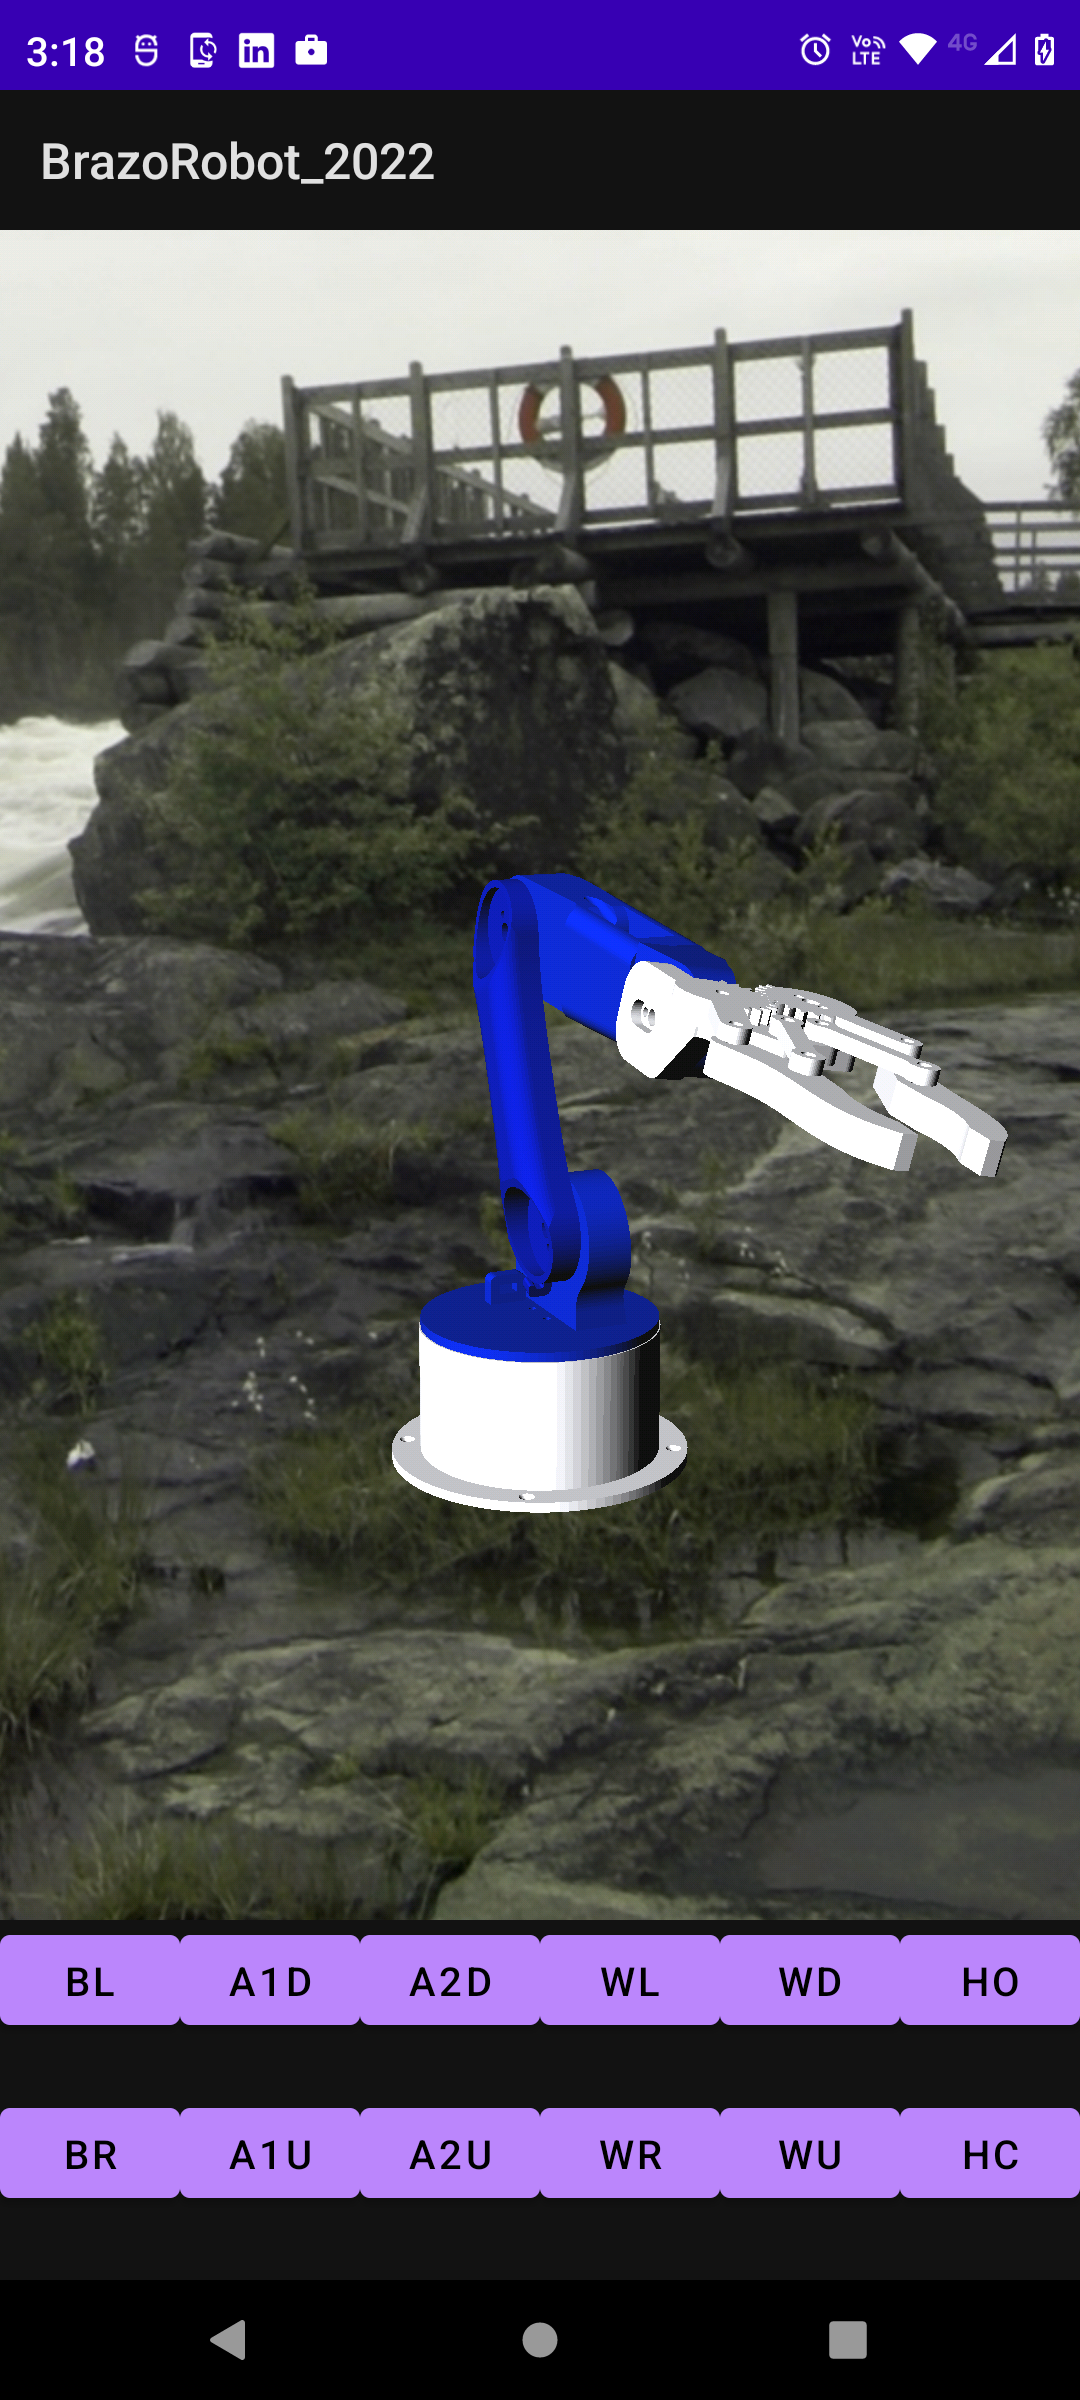
\includegraphics[width=0.82\textwidth]{2019_BrazoRobot3D/figs/BrazoRobot1}
\end{column}
\begin{column}{0.25\textwidth}  
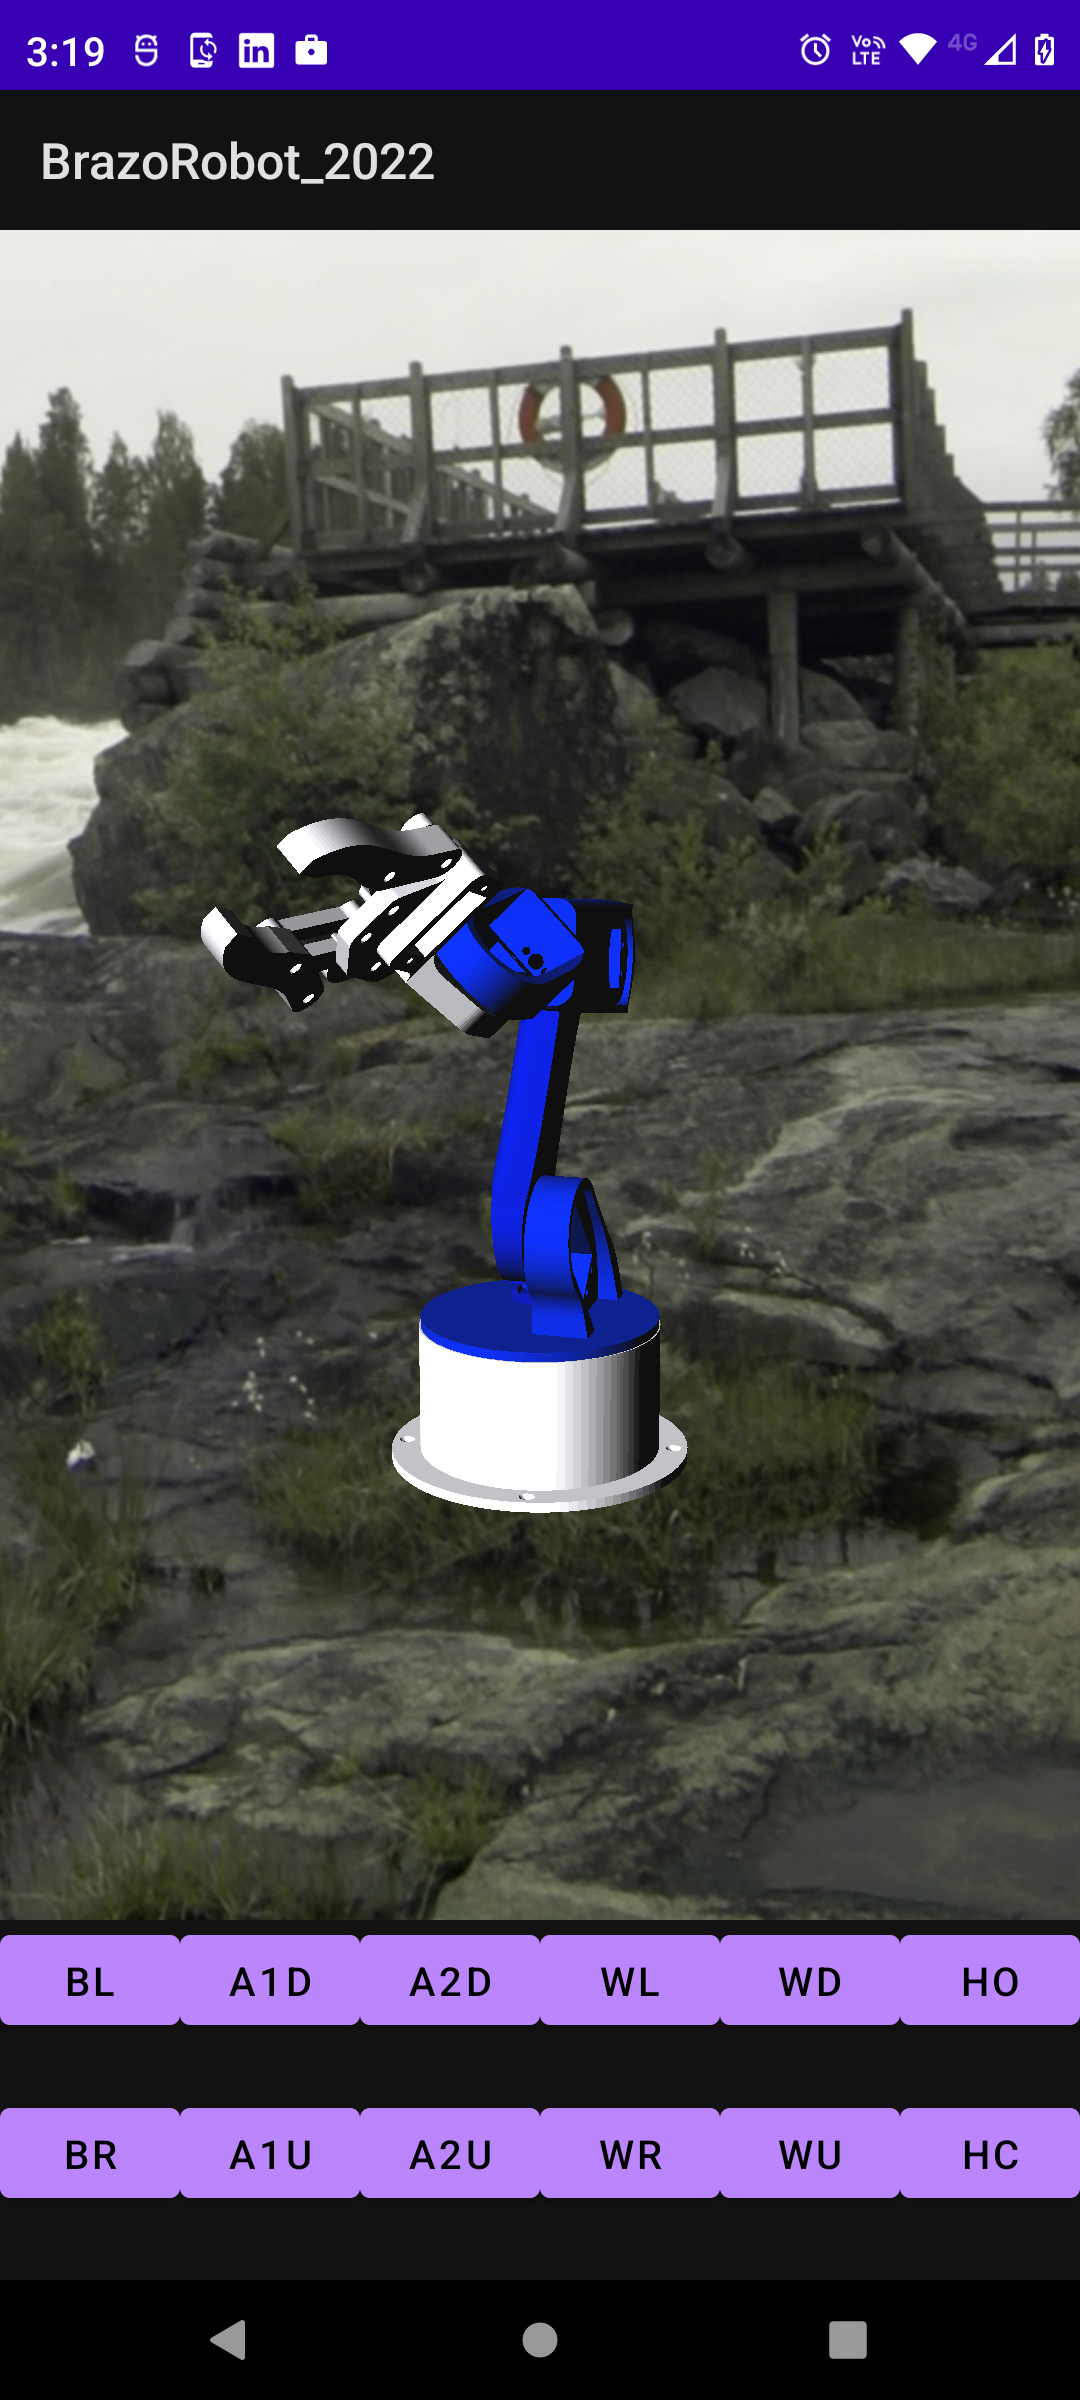
\includegraphics[width=0.82\textwidth]{2019_BrazoRobot3D/figs/BrazoRobot2}
\end{column}
\begin{column}{0.25\textwidth}  
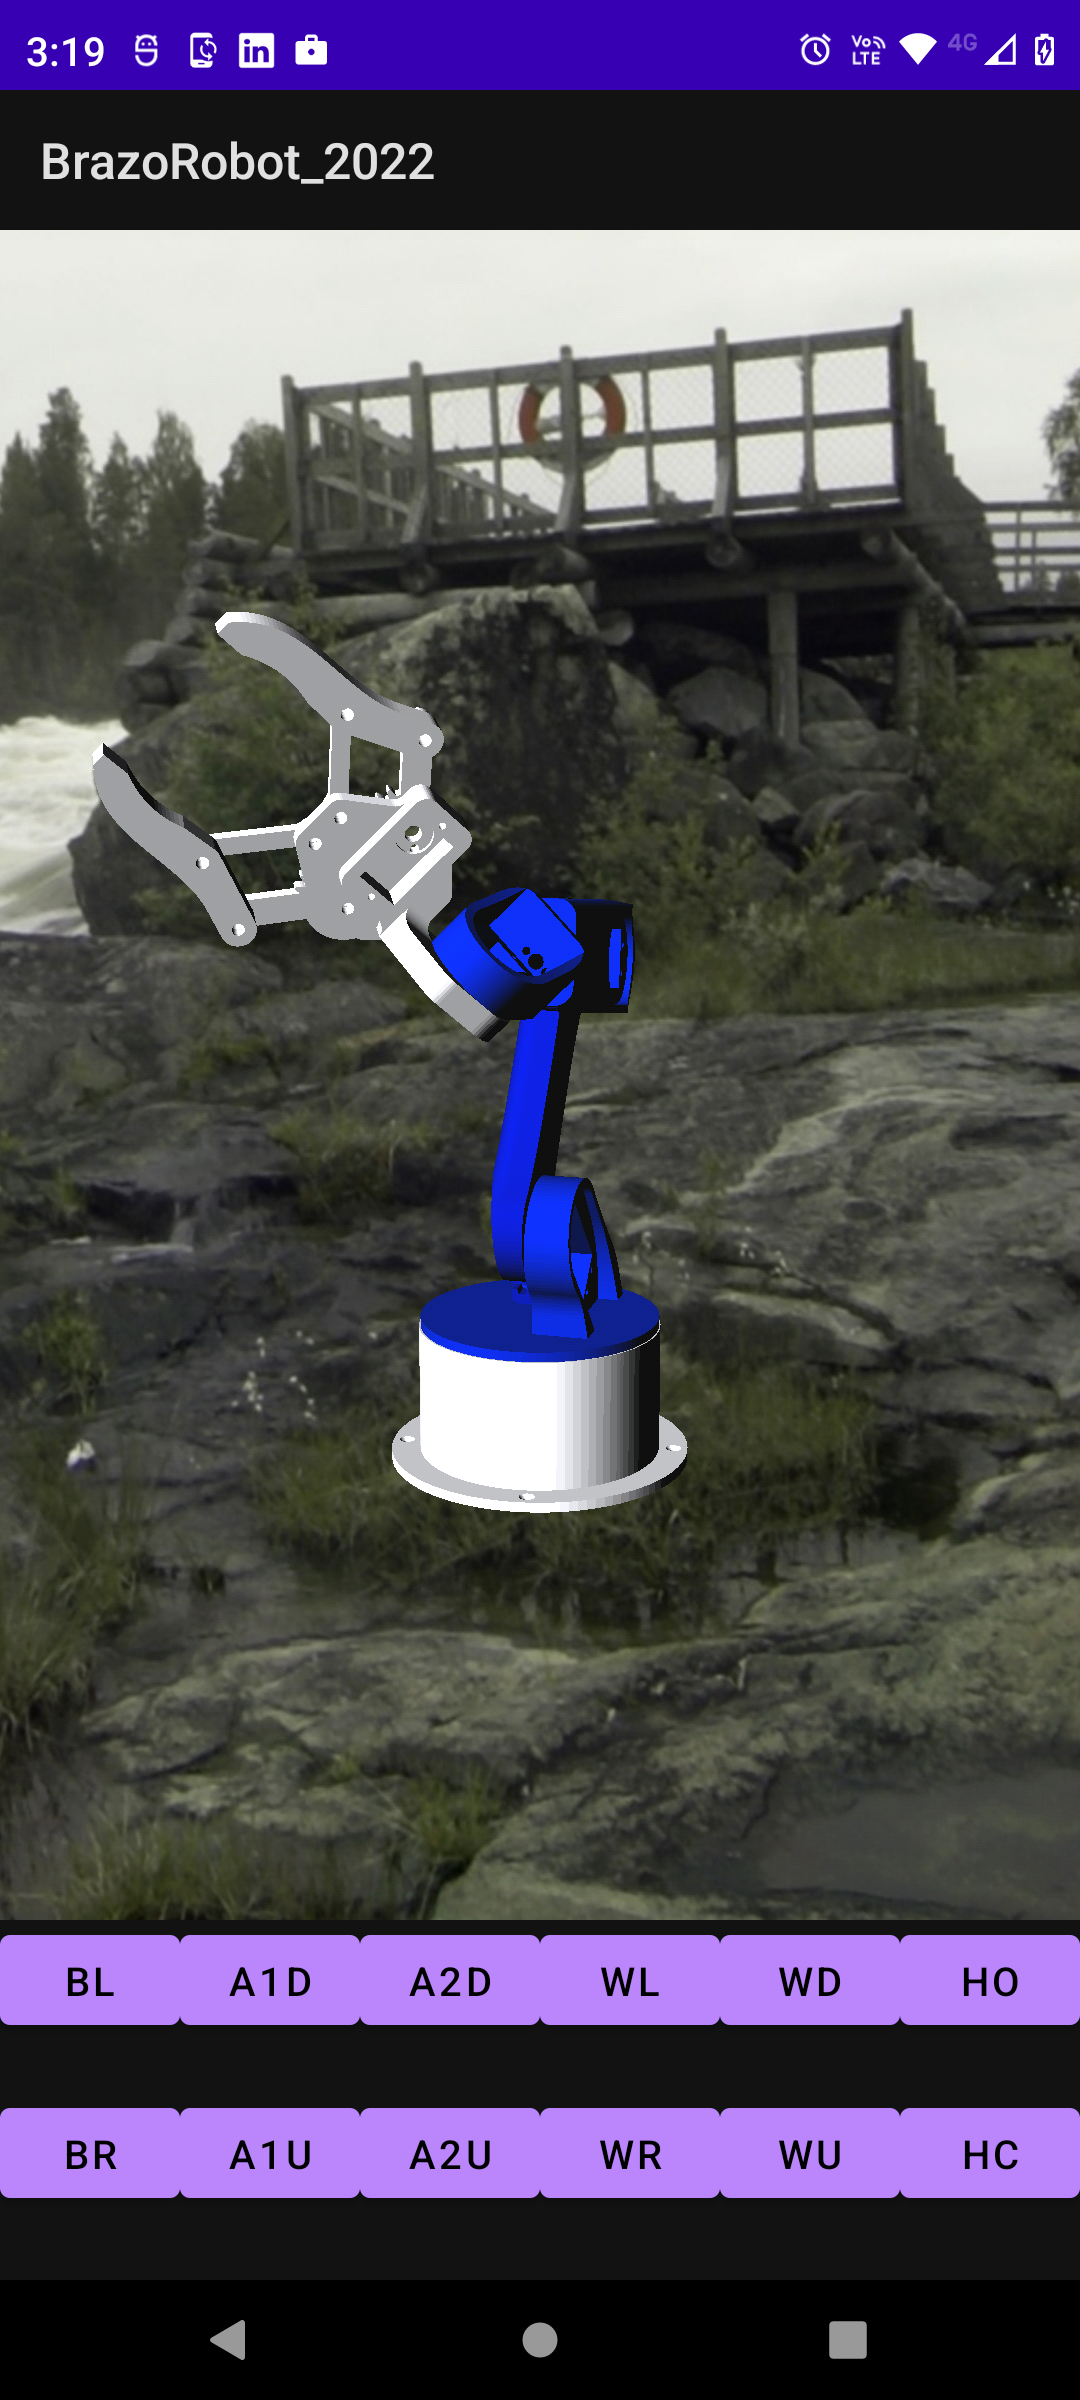
\includegraphics[width=0.82\textwidth]{2019_BrazoRobot3D/figs/BrazoRobot3}
\end{column}
\begin{column}{0.25\textwidth}  
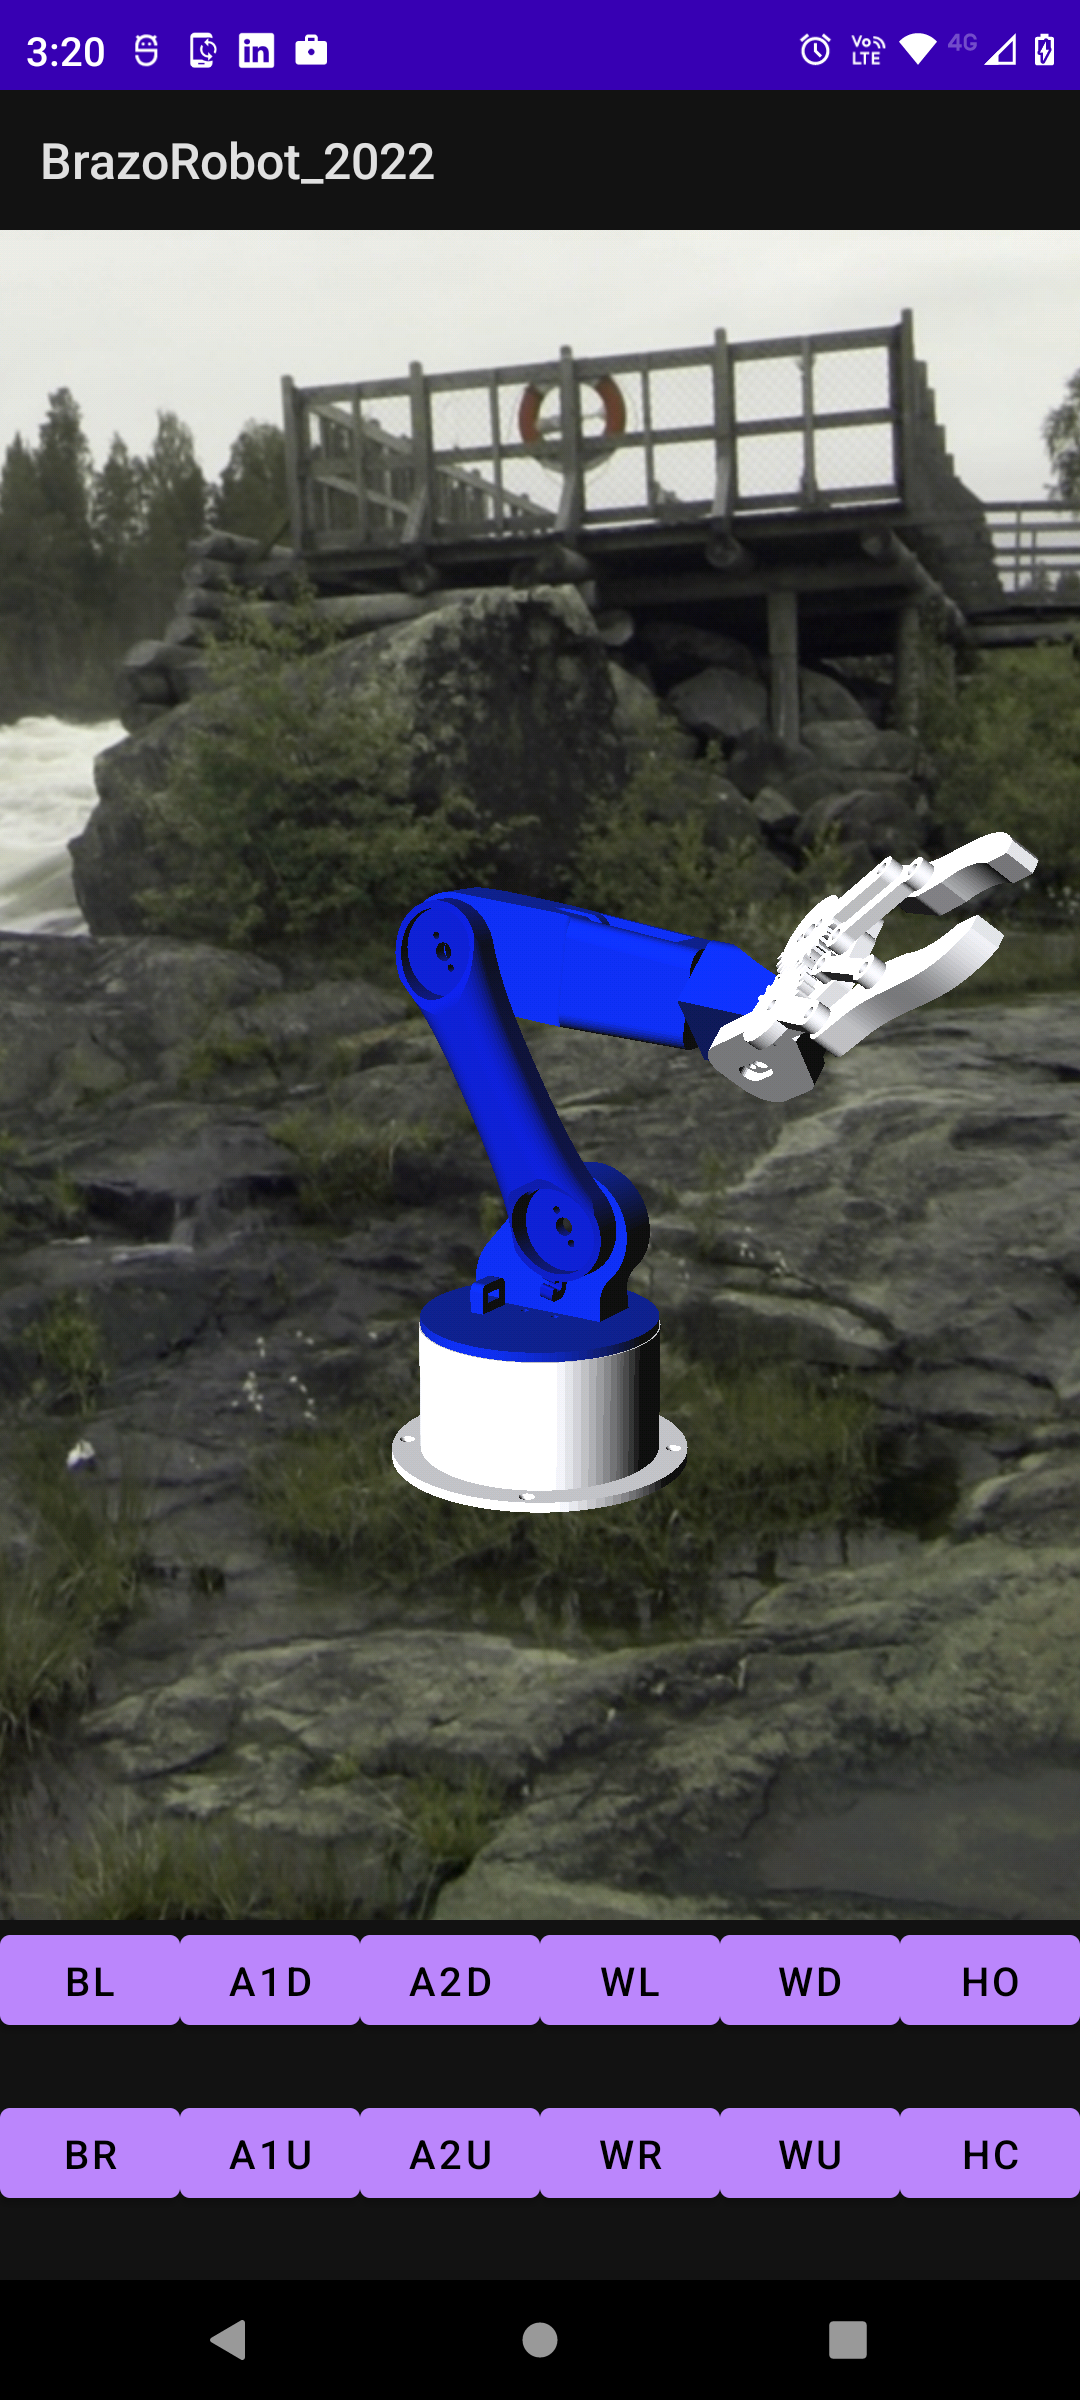
\includegraphics[width=0.82\textwidth]{2019_BrazoRobot3D/figs/BrazoRobot4}
\end{column}

\end{columns}
\footnotetext[1]{\fullcite{\EntradaBibtex}}
\end{frame}





\section[RV-TA]{Realidad Virtual y Aumentada}

% Diapositvias RV y RA

\begin{frame}{Realidad Aumentada (AR) \footnotemark}
%\begin{block}{Realidad Aumentada (AR) \footnotemark} 
\begin{columns}
\begin{column}{0.49\textwidth}
\begin{itemize}
\item La AR es una experiencia que traslapa elementos digitales (modelados por computadora) con el mundo físico del usuario (adquirido mediante una cámara). 
\item Los elementos digitales se combinan con las vistas del mundo real.
\end{itemize}
\end{column}
\begin{column}{0.49\textwidth}
\begin{center}
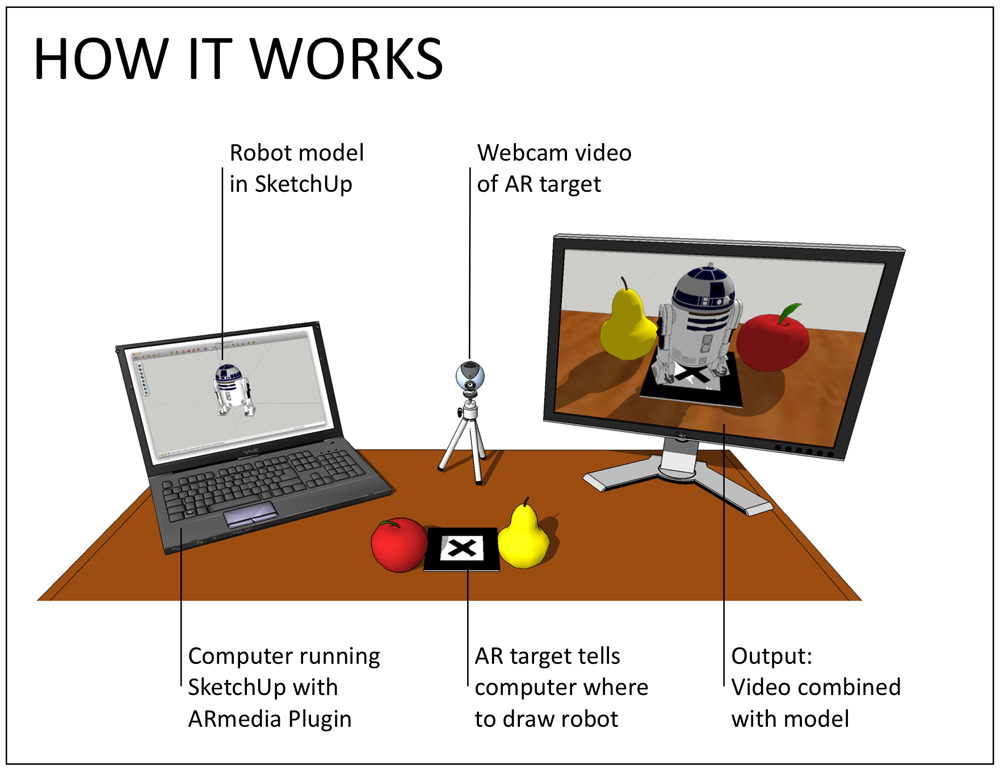
\includegraphics[width=0.95\textwidth]{Figs/AR_HowItWorks}
\end{center}
\end{column}
\end{columns}
\footnotetext{\url{http://photos1.blogger.com/img/m-a310d3b7b46f285189e1d6da63a1afd13be4ffc4.jpg}}
%\end{block} 
\end{frame}

\begin{frame}{Pasos en la detección de marcadores de AR \footnotemark}
%\begin{block}{Pasos en la detección de marcadores de AR \footnotemark} 
\begin{columns}
\begin{column}{0.39\textwidth}
\begin{enumerate}
\item Umbralización.
\item Detección del Marcador.
\item Estimación de Pose y Posición.
\item Empalme del modelo 3D.
\end{enumerate}
\end{column}
\begin{column}{0.59\textwidth}
\begin{center}
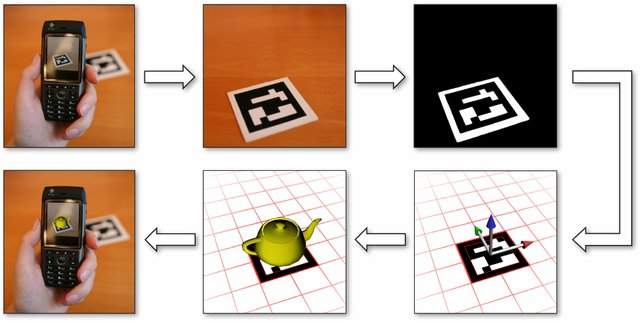
\includegraphics[width=0.95\textwidth]{Figs/AR_WorkFlow}
\end{center}
\end{column}
\end{columns}
%\end{block} 
\footnotetext{\fullcite{Wagner_ArToolKitPlus2007}}
\end{frame}


\begin{frame}{Tipos de Aplicación de AR \footnotemark}
%\begin{block}{Tipos de Aplicación de AR \footnotemark} 
\begin{columns}
\begin{column}{0.98\textwidth}
    \begin{center}

\begin{itemize}
\item Basadas en Localización. Están basada en sensores GPS para determinar la ubicación del dispositivo para crear objetos AR
\item Basadas en Visión – Utilizan una cámara, aunque también es posible incorporar sensores (compass, acelerómetros, giroscopios, etc). 
\begin{itemize}
\item  Requieren Marcadores (Marker) – Localizan un patrón o marcador QR  y renderizan un objeto 3D basado en su localización en el espacio real. 
\item  No requieren marcadores (Markerless)– Se emplean esquinas y puntos característicos del espacio real
\end{itemize}
\end{itemize}
     \end{center}

\end{column}
\end{columns}
%\end{block} 
\footnotetext{\url{https://fswa-net.com/index.php/news/use-of-ar-technology}}

%\\setcounter{footnote}{0}
\end{frame}


\begin{frame}{Aplicaciones de RA}
%\begin{block}{Aplicaciones de RA} 
\begin{itemize}
\item Aplicaciones principales: Arquitectura, Cosméticos, Contenido social, Marketing, Juegos, etc
\end{itemize}

\begin{columns}
\begin{column}{0.49\textwidth}
\begin{itemize}
\item Houzz
\end{itemize}
\begin{center}
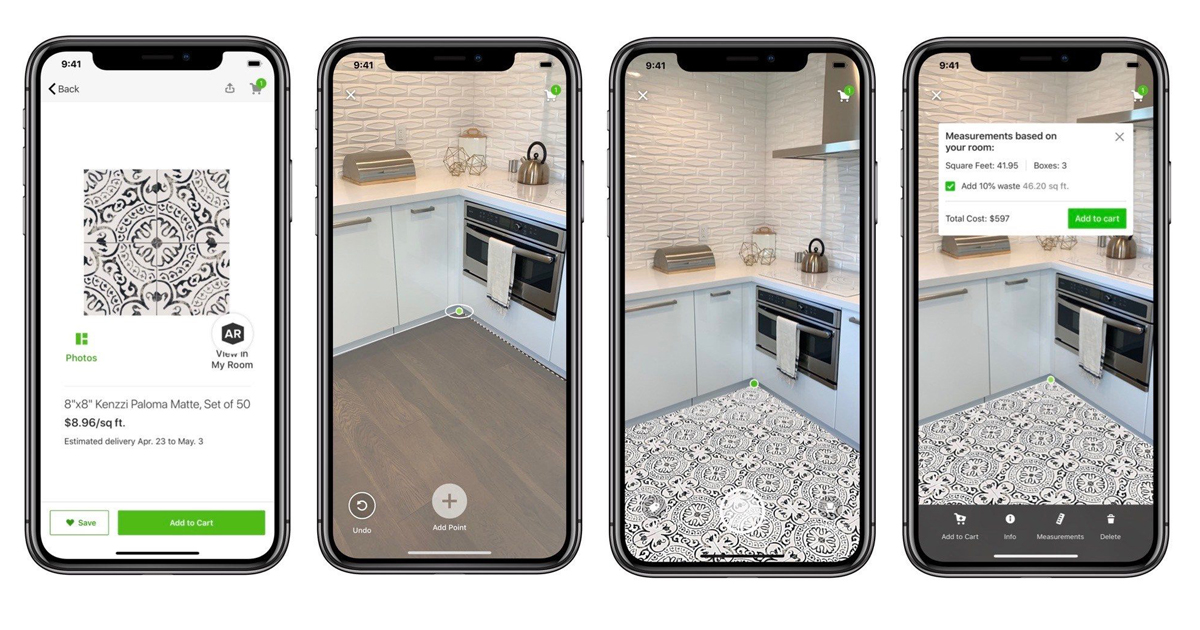
\includegraphics[width=0.9\textwidth]{Figs/AR_App}\\
\end{center}
\end{column}
\begin{column}{0.49\textwidth}  

\begin{itemize}
\item Pokemon Go
\end{itemize}
    \begin{center}
     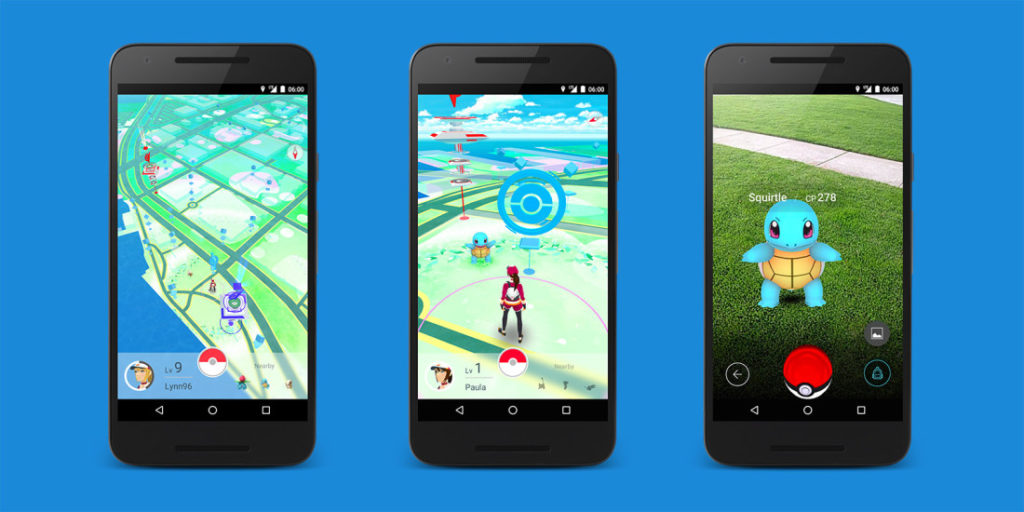
\includegraphics[width=0.9\textwidth]{Figs/Pokemon}
     \end{center}
\end{column}
\end{columns}
%\end{block} 
\end{frame}


\begin{frame}{Realidad Virtual - Antecedente hist\'orico}

\begin{columns}
\begin{column}{0.49\textwidth}


\begin{itemize}
\item Un estereoscopio proporciona im\'agenes separadas para cada ojo mediante lentes individuales, donde cada imagen tiene una variante en el angulo de captura y un desplazamiento horizontal.
\item El cerebro de una persona con una percepción binocular normal de la profundidad al utilizar el estereoscopio ``mezcla'' ambas imagenes para crear una  ``ventana estereoscópica''
\end{itemize}
\end{column}

\begin{column}{0.49\textwidth}

\begin{center}
	\begin{tabular}{cc}
        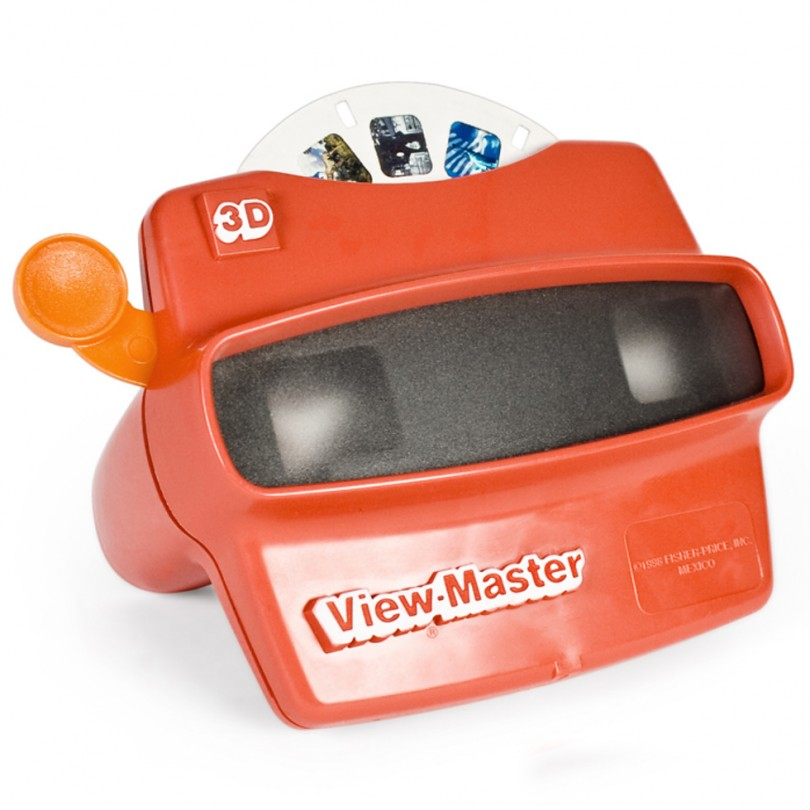
\includegraphics[width=0.45\linewidth]{Figs/view_master_blog-810x810.jpg} &
		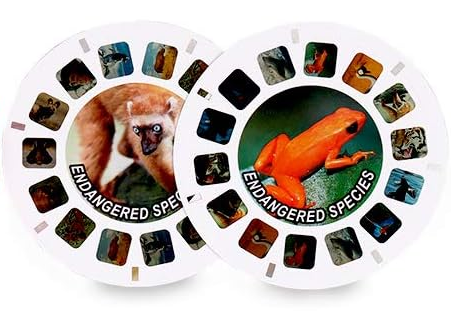
\includegraphics[width=0.45\linewidth]{Figs/DiscosViewMaster.png}    
	\end{tabular}

	\begin{tabular}{cc}
	\centering
        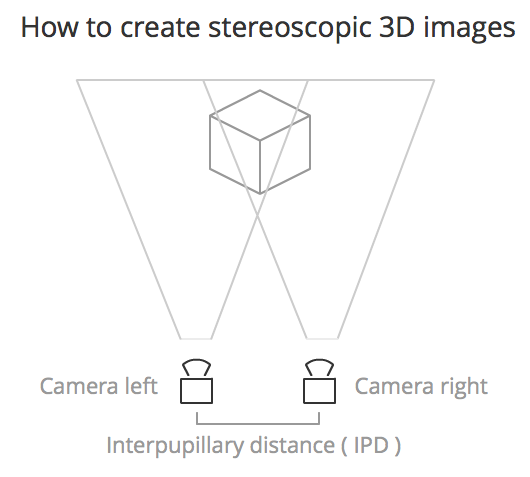
\includegraphics[width=0.49\linewidth]{Figs/VirtualReal1} &
        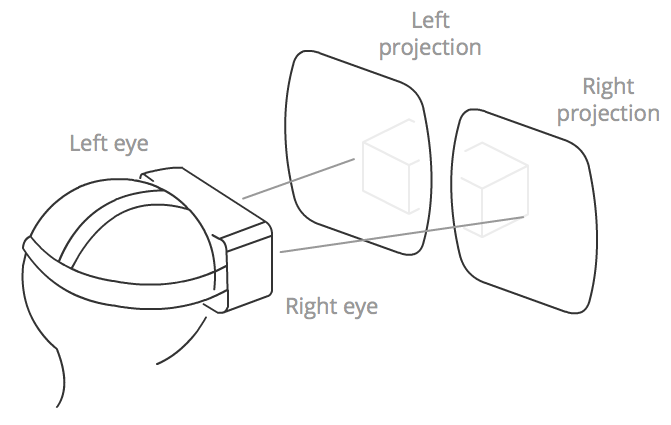
\includegraphics[width=0.49\linewidth]{Figs/VirtualReal2} \\

	\end{tabular}
\end{center}
\end{column}

\end{columns}

\end{frame}




\begin{frame}{Realidad Virtual (VR)}
%\begin{block}{Realidad Virtual (VR)} 
		\begin{itemize}
			\item La Realidad virtual (RV) emplea modelos y simulaciones por computadora que permite a una persona interactuar con un entorno visual artificial tridimensional (3D)
			\item En un formato típico de RV, un usuario lleva un casco con una pantalla estereoscópica para ver imágenes animadas de un entorno simulado
			\item El dispositivo m\'as econ\'omico para aplicaciones de RV es un tel\'efono inteligente 
		\end{itemize}
    \begin{center}
	\begin{tabular}{ccc}
    	\centering
		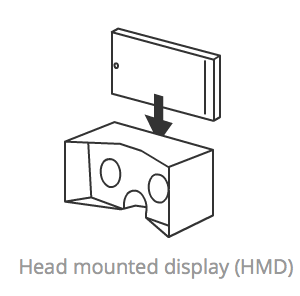
\includegraphics[width=0.25\linewidth]{Figs/MobileVR2} & 
        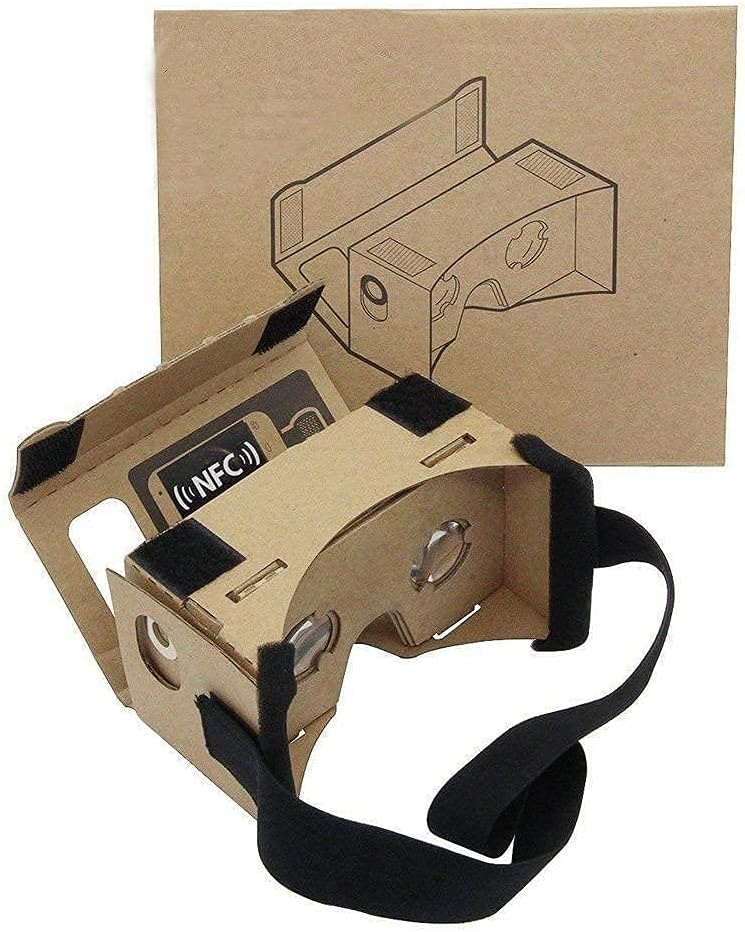
\includegraphics[width=0.19\linewidth]{Figs/CardBoard} & 		
        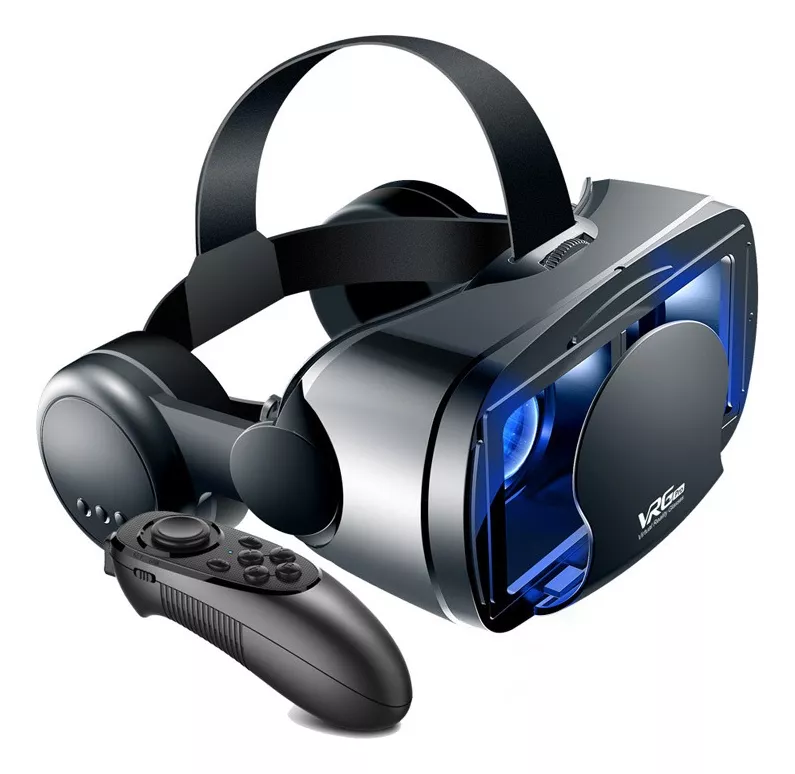
\includegraphics[width=0.19\linewidth]{Figs/VRGPro} 		
	\end{tabular}
		 \end{center}
%\end{block} 
\footnotetext{\url{https://reference.codeproject.com/book/dom/webvr_api/webvr_concepts}}
\end{frame}


\begin{frame}{Costos de Dispostivos HeadSets para VR}
\begin{columns}
\begin{column}{0.49\textwidth}
\begin{itemize}
\item Meta Quest 3 (499 USD)
\item Sony PlayStation VR2 (599 USD)
\item Meta Quest Pro (900 USD)
\item Valve Index VR Kit (1350 USD)
\item HTC Vive Pro 2 (1400 USD)
\end{itemize}

\begin{center}
\includegraphics[width=0.75\textwidth]{Figs/sony.png}
\end{center}
\end{column}
\begin{column}{0.49\textwidth}
\begin{center}
\includegraphics[width=0.75\textwidth]{Figs/HTC.jpg}\\
\includegraphics[width=0.95\textwidth]{Figs/MetaPro.jpg}
\end{center}
\end{column}
\end{columns}
\end{frame}


\begin{frame}{Relación entre RA/RV - Teléfonos Inteligentes}
Los teléfonos inteligentes son una de las principales plataformas para sistemas de \textbf{realidad aumentada (AR) y realidad virtual (VR)}:  
\begin{itemize}
\item Tienen hardware avanzado (cámaras, sensores de movimiento, procesadores gráficos) que permiten ejecutar experiencias inmersivas de AR y VR sin necesidad de equipos especializados.  
\item Existen accesorios como **gafas VR para móviles** (ej. Google Cardboard, Samsung Gear VR) que convierten un teléfono en un visor de realidad virtual.  
\item Existen herramientas para crear apps de RA y RV
\item Muchas aplicaciones combinan AR con inteligencia artificial para ofrecer experiencias interactivas y personalizadas.  
\item Gran cantidad de aplicaciones prácticas
\end{itemize}
\end{frame}


\renewcommand{\EntradaBibtex}{MarcoNuno_Revista_2018_08_00}
\begin{frame}{\citetitle{\EntradaBibtex} \footnotemark[1] (1)}


%\begin{frame}{\citetitle{MarcoNuno_Revista_2018_08_00} \footnotemark (1)}
%\begin{block}{Aplicación para Enseñanza de Robótica utilizando Realidad Aumentada \footnotemark (1)} 
\begin{columns}
\begin{column}{0.5\textwidth}
Componentes:
		\begin{itemize}
		\item Un sistema (Arduino) que genera los movimientos del brazo robot incluye un transmisor Bluetooth
		\item Una aplicación móvil que visualizar un transportador virtual encima de una articulación robótica con el ángulo en tiempo real
		\end{itemize}
\end{column}
\begin{column}{0.5\textwidth}  
    \begin{center}
     %%%%% this is a minipage, so \textwidth is already adjusted to the size of the column
     \includegraphics[width=0.9\textwidth]{Figs/SistemaAR_Maestria1}
     \end{center}
\end{column}
\end{columns}
%\end{block} 
\footnotetext[1]{\fullcite{\EntradaBibtex}}

\end{frame}

\begin{frame}{\citetitle{\EntradaBibtex} (2)}
%\begin{block}{Aplicación para Enseñanza de Robótica utilizando Realidad Aumentada (2)} 
\begin{columns}
\begin{column}{0.5\textwidth}
Funcionamiento de la aplicación:
		\begin{itemize}
		\item Se emplea un marcador ARUCO para determinar de que articulación se trata
		\item Mediante comandos Bluetooth se obtiene el ángulo
		\end{itemize}
\begin{center}
     %%%%% this is a minipage, so \textwidth is already adjusted to the size of the column
     \includegraphics[width=0.79\textwidth]{Figs/SistemaAR_Maestria2}
     \end{center}
\end{column}
\begin{column}{0.5\textwidth}  
    \begin{center}
     %%%%% this is a minipage, so \textwidth is already adjusted to the size of the column
     \includegraphics[width=0.79\textwidth]{Figs/SistemaAR_Maestria3}
     \includegraphics[width=0.79\textwidth]{Figs/SistemaAR_Maestria4}
     \end{center}
\end{column}
\end{columns}
%\end{block} 
\end{frame}




\renewcommand{\EntradaBibtex}{RealidadAumentada_PrimerPrototipo_2019}
\begin{frame}{\citetitle{\EntradaBibtex} \footnotemark[1] (1)}

%\begin{frame}{Sistema de Realidad Aumentada \footnotemark}
%\begin{block}{Sistema de Realidad Aumentada \footnotemark} 
\begin{columns}
\begin{column}{0.48\textwidth}
		\begin{itemize}
		\item Detección de Codigos QR
		\item Decodificación del texto codificado en el codigo QR
		\item Sobreposición del modelo 3D dependiendo de la posición del código QR
		\end{itemize}
	\end{column}
	\begin{column}{0.52\textwidth}  
	    \begin{center}
	    	 \includegraphics[width=0.95\textwidth]{Figs/SistemaAR1}
    	 \end{center}
	\end{column}
	\end{columns}
%	\end{block} 
\footnotetext[1]{\fullcite{\EntradaBibtex}}
%\footnotetext{Cárdenas Castillo Jesús Alfredo, Molina Pastrana Ana Karen, Ramos Lucio Eluis Carlo, Rodríguez Terán Linda Margarita y Vázquez Luna César Jovany.  \textbf{Visión por Computadora para Realidad Aumentada}. Universidad Politécnica de Victoria,  Informe técnico proyecto de asignatura ``Cómputo en Dispositivos Móviles'', 2019. Sin Publicar.}
%\\setcounter{footnote}{0}
\end{frame}

%Cárdenas Castillo Jesús Alfredo, Molina Pastrana Ana Karen, Ramos Lucio Eluis Carlo, Rodrı́guez Terán Linda Margarita, Vázquez Luna Cesar Jovany.
% \textbf{Visión por Computadora para Realidad Aumentada}. Universidad Politécnica de Victoria,  Informe técnico proyecto de asignatura ``Cómputo en Dispositivos Móviles'', 2019. Sin Publicar.

\begin{frame}{\citetitle{\EntradaBibtex} (2)}
%\begin{block}{Sistema de Realidad Aumentada (2)} 
\begin{columns}
\begin{column}{0.5\textwidth}
    \begin{center}
\includegraphics[width=0.98\textwidth]{Figs/SistemaAR2}\\
     \end{center}

\end{column}
\begin{column}{0.5\textwidth}  
    \begin{center}
\begin{itemize}
\end{itemize}

\includegraphics[width=0.98\textwidth]{Figs/SistemaAR3}\\
     \end{center}
\end{column}
\end{columns}



%\end{block} 
\end{frame}


\renewcommand{\EntradaBibtex}{JaguarAplicacionMovil_2020}
\begin{frame}{\citetitle{\EntradaBibtex} \footnotemark[1] (1)}


%\begin{frame}{Desarrollos Tecnológicos}
\begin{block}{-} 
\begin{columns}
\begin{column}{0.48\textwidth}
		\begin{itemize}
		\item Detección de Codigos QR
		\item Modelado de la mascota en 3D mediante el Software Blender
		\item Sobreposición del modelo 3D dependiendo de la posición del código QR
		\end{itemize}
	\end{column}
	\begin{column}{0.52\textwidth}  
	    \begin{center}
	    	 \includegraphics[width=0.25\textwidth]{Figs/JaguarFisico01}
	    	 \includegraphics[width=0.25\textwidth]{Figs/JaguarFisico02}\\
    	 \end{center}
	\end{column}
	\end{columns}
	\end{block} 
	%\footnotetext{\fullcite{JaguarAplicacionMovil_2020}}
\footnotetext[1]{\fullcite{\EntradaBibtex}}
%\footnotetext{Andrés García González, Cristian Aléxis Lazo García, Damaris Mendoza Vázquez.  \textbf{Modelo 3D del Jaguar de la UPV sobre un código QR}. Universidad Politécnica de Victoria,  Informe técnico proyecto de asignatura ``Graficación por Computadora Aavanzada'', 2020. Sin Publicar.}
%\\setcounter{footnote}{0}
\end{frame}


\begin{frame}{\citetitle{\EntradaBibtex} (2)}
\begin{block}{-} 
\begin{columns}
	\begin{column}{0.98\textwidth}
	    \begin{center}
	    	 \includegraphics[width=0.24\textwidth]{Figs/JaguarVirtual01}
	    	 \includegraphics[width=0.24\textwidth]{Figs/JaguarVirtual02}
	    	 \includegraphics[width=0.24\textwidth]{Figs/JaguarVirtual03}
	    	 \includegraphics[width=0.24\textwidth]{Figs/JaguarVirtual04}
    	 \end{center}
	\end{column}
	\end{columns}
	\end{block} 
\end{frame}



\begin{frame}{Recorrido UPV Virtual en teléfonos inteligentes}
%\begin{block}{Recorrido UPV Virtual en teléfonos inteligentes} 
Demo incremental, que emplea OpenGL ES 2.0 (compatible con el 100\% de los smartphones). 
\begin{itemize}
\item Versión 1: Solo mundo virtual (no inmersivo). El usuario se movía con presionando teclas de la interfaz de usuario
\item Versión 2: Mundo virtual inmersivo (integrado a unos lentes). El usuario movía la vista mediante los datos obtenidos por el sensor giroscopio del teléfono inteligente y avanzaba usando un manos libres alámbrico.
\item Versión 3: Controlado por voz. El usuario se movía dentro del entorno mediante comandos de voz.
\item Versión 3.5: Controlado mediante control de videojuegos (Bluetooth o USB)
\end{itemize}
%\end{block} 
\end{frame}

\renewcommand{\EntradaBibtex}{Reporte2019}
\begin{frame}{\citetitle{\EntradaBibtex} \footnotemark[1] (1)}

%\begin{frame}{Recorrido UPV Virtual 1.0\footnotemark }
%\begin{block}{} 
\begin{columns}
\begin{column}{0.48\textwidth}
    \begin{center}

\begin{itemize}
\item La navegación es mediante botones (adelante, atrás, izquierda, derecha, subir, bajar)
\item Una potencial mejora es mediante eventos de toque en pantalla
\end{itemize}
     \end{center}

\end{column}
\begin{column}{0.52\textwidth}  
    \begin{center}
\begin{itemize}
\end{itemize}
     \includegraphics[width=0.9\textwidth]{Figs/RecorridoUPV_V1}\\
     \end{center}
\end{column}
\end{columns}
%\end{block} 
\footnotetext[1]{\fullcite{\EntradaBibtex}}
%\footnotetext{Baez Zapata Marıa Fernanda, Cárdenas Castillo Jesús Alfredo, Olvera Osuna José Armando and Wang Yu Hsiang. \textbf{Recorrido UPV en Android}. Proyecto Final de la Asignatura ``Cómputo en Dispositivos Móviles'', 2019. Sin Publicar.}
%\\setcounter{footnote}{0}
\end{frame}


%\begin{frame}{Recorrido UPV Virtual 1.0 (2)}
%\renewcommand{\EntradaBibtex}{Reporte2019}
\begin{frame}{\citetitle{\EntradaBibtex}  (2)}
%\begin{block}{Recorrido UPV Virtual 1.0 (2)} 
\begin{itemize}
\item Vistas de los diferentes edificios
\end{itemize}
    \begin{center}
     \includegraphics[width=0.80\textwidth]{Figs/RecorridoUPV_V2}\\
     \end{center}
%\end{block} 
\end{frame}

\renewcommand{\EntradaBibtex}{RecorridoVirtualLentesVR_2019}
%\begin{frame}{Recorrido UPV Virtual 2.0\footnotemark}
\begin{frame}{\citetitle{\EntradaBibtex}  (2)}
%\begin{block}{Recorrido UPV Virtual 2.0\footnotemark} 
\begin{columns}
\begin{column}{0.48\textwidth}
    \begin{center}

\begin{itemize}
\item Se extendió el demo 1.0 para generar una vista dual, requerida para su uso en conjunto con un armazón de VR.
\item La vista cambia en base a lo obtenido por el giroscopio, y el movimiento se controla mediante el botón del manos libres.
\end{itemize}
     \end{center}

\end{column}
\begin{column}{0.52\textwidth}  
    \begin{center}
\begin{itemize}
\end{itemize}
     \includegraphics[width=0.4\textwidth]{Figs/RecorridoUPV_V3}\\
     \end{center}
\end{column}
\end{columns}
%\end{block} 
%\footnotetext{\fullcite{RecorridoVirtualLentesVR_2019}}
\footnotetext[1]{\fullcite{\EntradaBibtex}}
%\footnotetext{Alarcon Longoria Carlos Alberto, Alonso Cepeda Leonardo Daniel and Torres Grimaldo Luis Angel. \textbf{Recorrido UPV Virtual en Android}.  Proyecto Final de la Asignatura ``Cómputo en Dispositivos Móviles'', 2019. Sin Publicar.}
%\\setcounter{footnote}{0}
\end{frame}


\renewcommand{\EntradaBibtex}{RecorridoVirtualLentes_ComandosVoz2020}
\begin{frame}{\citetitle{\EntradaBibtex}  (1)}
%\begin{block}{Recorrido UPV Virtual 3.0\footnotemark} 
\begin{columns}
\begin{column}{0.48\textwidth}
    \begin{center}
\begin{itemize}
\item Se eliminó el uso del botón del manos libres para incluir comandos de voz
\item La aplicación respondía a los comandos de voz, de tal forma que el usuario no debería mover nada
\end{itemize}
     \end{center}

\end{column}
\begin{column}{0.52\textwidth}  
    \begin{center}
     \includegraphics[width=0.6\textwidth]{Figs/RecorridoUPV_V5}\\
     \end{center}
\end{column}
\end{columns}
%\end{block} 
\footnotetext[1]{\fullcite{\EntradaBibtex}}
%\footnotetext{José Treviño Olvera. \textbf{Recorrido UPV Virtual en Android con Controles de Voz.}  Proyecto Final de la Asignatura. ``Cómputo en Dispositivos Móviles'', 2020. Sin Publicar.}
%\\setcounter{footnote}{0}
\end{frame}

\renewcommand{\EntradaBibtex}{RecoridoUPV_controles_2021}
%\begin{frame}{Recorrido UPV Virtual 3.5 \footnotemark}
%\begin{block}{Recorrido UPV Virtual 3.5 \footnotemark } 
\begin{frame}{\citetitle{\EntradaBibtex}  (1)}
\begin{itemize}
\item Se incorporaron varios controles de consolas de videojuego para la navegación.
\end{itemize}
\begin{columns}
\begin{column}{0.48\textwidth}
\begin{center}
	\begin{tabular}{ccc}
		\includegraphics[width=0.25\linewidth]{Figs/UPV_Control01} & 		
		\includegraphics[width=0.25\linewidth]{Figs/UPV_Control02} & 
        \includegraphics[width=0.25\linewidth]{Figs/UPV_Control04}\\
	\end{tabular}
\end{center}
\end{column}
\begin{column}{0.48\textwidth}
\begin{center}
	\begin{tabular}{c}
		    \includegraphics[width=0.45\linewidth]{Figs/UPV_Control03}\\
		    \includegraphics[width=0.45\linewidth]{Figs/UPV_Control05}\\
	\end{tabular}
\end{center}	
\end{column}
\end{columns}
%\end{block} 
\footnotetext[1]{\fullcite{\EntradaBibtex}}
%\footnotetext{\fullcite{RecoridoUPV_controles_2021}}
\end{frame}



\renewcommand{\EntradaBibtex}{CabezaJaguar_2023}
\begin{frame}{\citetitle{\EntradaBibtex} \footnotemark[1] (1)}
%\begin{block}{Brazo Robótico \footnotemark} 
\begin{columns}
	\begin{column}{0.55\textwidth}
		\begin{itemize}
			\item La mascota institucional de la UPV es el Jaguar
			\item Se diseño un filtro que detecta el rostro de una persona y sobrepone la imagen de un Jaguar
		\end{itemize}
	\end{column}
	\begin{column}{0.22\textwidth}
		 \begin{center}
		     \includegraphics[width=0.98\textwidth]{2025_CabezaJaguarUPV/figs/Jaguar1}
		 \end{center}
	\end{column}
	\begin{column}{0.22\textwidth}  
		\begin{center}
		 \includegraphics[width=0.98\textwidth]{2025_CabezaJaguarUPV/figs/Jaguar2}
		 \end{center}
	\end{column}
\end{columns}
%\end{block} 
\footnotetext[1]{\fullcite{\EntradaBibtex}}
\end{frame}




\renewcommand{\EntradaBibtex}{MapaRAChidoUPV_2023}
\begin{frame}{\citetitle{\EntradaBibtex} \footnotemark[1] (1)}
%\begin{block}{Brazo Robótico \footnotemark} 
\begin{columns}
	\begin{column}{0.55\textwidth}
		\begin{itemize}
			\item Se diseñó una aplicación de Realidad Aumentada que muestra un mapa de la UPV
			\item Se modeló el mapa en Blender y se integró a la aplicación
		\end{itemize}
	\end{column}
	\begin{column}{0.44\textwidth}
		 \begin{center}
		     \includegraphics[width=0.98\textwidth]{2025_MapaRA_UPV/figs/1}
		 \end{center}
	%\end{column}
	%\begin{column}{0.22\textwidth}  
		\begin{center}
		 \includegraphics[width=0.98\textwidth]{2025_MapaRA_UPV/figs/2}
		 \end{center}
	\end{column}
\end{columns}
%\end{block} 
\footnotetext[1]{\fullcite{\EntradaBibtex}}
\end{frame}





\section[VCyAA]{Visión por Computadora y Aprendizaje Automático}

% Diapositvias VC

\begin{frame}{Visión por Computadora}
%\begin{block}{Fundamentación} 
\begin{columns}
\begin{column}{0.60\textwidth}
    \begin{center}
\begin{itemize}
\item La visión por computadora imita la percepción humana y las capacidades de razonamiento.
\item Se intenta inferir conocimiento a partir de imágenes o videos.
\item Procesamiento de imágenes es una fase temprana de la VC. La entrada es una imagen y la salida es otra imagen.
\item En la visión por computadora, la entrada es una imagen pero la salida son datos. 
\end{itemize}
     \end{center}

\end{column}
\begin{column}{0.40\textwidth}  
    \begin{center}
     \includegraphics[width=0.9\textwidth]{Figs/VC}
     \end{center}
\end{column}
\end{columns}
%\end{block} 
\end{frame}

\begin{frame}{Visión por Computadora (Detección de Bordes) (II)}
  \begin{columns}
  \column {0.4\textwidth}
  \begin{itemize}
    \item La información acerca de bordes es útil para entender el ambiente.
    \item Las esquinas son primitivas que permiten identificar limites y puntos de interés dentro de la geometría de las imágenes.
  \end{itemize}  
      \column {0.3\textwidth}  
        \begin{center}
            \includegraphics[width=\textwidth]{Figs/VC_CocaOrig}\\
     \end{center}
      
    \column {0.3\textwidth}  
        \begin{center}
            \includegraphics[width=\textwidth]{Figs/VC_CocaBordes}
     \end{center}

    \end{columns}

\end{frame}

\begin{frame}{Visión por Computadora (Segmentación) (II)}
\begin{columns}
  \column {0.8\textwidth}
  \begin{itemize}
    \item Localizar y aislar objetos de interés en la imagen.
    \item Localización de Objetivos, navegación, conteo de objetos
    \item Algoritmos de segmentación en escala de grises. Segmentación global (un umbral común para toda la imagen y segmentación local (umbrales múltiples en regiones de la imágen).
    \item Algoritmos de segmentación por color: muy utilizados para detectar la piel y encontrar partes del cuerpo.
  \end{itemize}
  
    \column {0.2\textwidth}  
        \begin{center}
            \includegraphics[width=\textwidth]{Figs/VC_Segmentacion}\\
     \end{center}

    \end{columns}
\end{frame}

\begin{frame}{Visión por Computadora (Template Matching) (II)}

Permite comparar imágenes aplicando operaciones de comparación entre regiones.
\begin{columns}
  \column {0.5\textwidth}
  \begin{itemize}
    \item Algoritmos clásicos basados en correlación: SAD, SSD, Rank.
	  \begin{itemize}
		    \item Ventajas: Facil de entender, rápidos
		    \item Desventajas: Sensibles a la escala, a rotaciones y a cambios en la iluminación. 
	  \end{itemize}
    \item Algoritmos modernos basados Aprendizaje Profundo
		\begin{itemize}
		    \item Ventajas: Buen desempeño 
		    \item Desventajas: Requieren de entrenamiento con muchas imágenes
	  \end{itemize}

  \end{itemize}
    \column {0.5\textwidth}  
        \begin{center}
            \includegraphics[width=\textwidth]{00_IntroComputerVision/figs/Industrial-software-example-for-Template-Matching_W640}\\
     \end{center}

    \end{columns}
\end{frame}




%\subsection{Redes Neuronales}

\begin{frame}{Aprendizaje Máquina (Machine Learning)}

Es una disciplina de la IA que por medio de \textbf{algoritmos y datos}, permite a las computadoras imitar la forma en la que los humanos aprenden, mejorando su precisión de manera gradual
\begin{columns}
\begin{column}{0.48\textwidth}
\begin{itemize}
\item Aprendizaje Supervisado: se requiere tener conocimiento previo de etiquetas asignadas a los datos para poder generar el modelo
\item Aprendizaje No supervisado: intentan descubrir patrones ocultos o agrupamientos de datos sin requerir de intervención humana
\end{itemize}
\end{column}
\begin{column}{0.52\textwidth}  
    \begin{center}
     \includegraphics[width=\textwidth]{00_IntroMachineLearning/figs/Classifier}
     \end{center}
\end{column}
\end{columns}


\end{frame}

\begin{frame}{Aprendizaje Máquina vs Aprendizaje Profundo}
%\Huge

	%\begin{block}{Aprendizaje Máquina} 
		\begin{columns}
		\begin{column}{0.57\textwidth}
		\begin{block}{Aprendizaje Máquina} 
		\begin{itemize}
		\item Se requiere de una fase de \textbf{extracción de características} de los datos de entrada
		\item Existen múltiples algoritmos, uno de los más representativos son las Redes Neuronales
		\end{itemize}
		\end{block} 
        \begin{block}{Aprendizaje Profundo} 
		\begin{itemize}
		\item La fase de \textbf{extracción de características} no es necesaria
        \item Principalmente basadas en redes neuronales
%		\item Una generación de algoritmos que permiten resolver tareas.
		%\item Las computadoras intentan resolver tareas que solo son posibles mediante inteligencia humana
		%\item Es una rama muy amplia que cubre muchos aspectos de la vida cotidiana.
		\end{itemize}
		\end{block} 

		\end{column}
		\begin{column}{0.37\textwidth}  
			\begin{center}
			 \includegraphics[width=\textwidth]{Figs/MachineLearningVsDeepLearning}
			 %\includegraphics[width=\textwidth]{WordReading2}
			 \end{center}
		\end{column}
	\end{columns}
	%\end{block} 
\end{frame}



\renewcommand{\EntradaBibtex}{AppComidaTamaulipeca_SistemasInteligentes_UPV_2023}


\begin{frame}{\citetitle{\EntradaBibtex} \footnotemark[1] (1)}
\begin{block}{Motivación} 
Desarrollar aplicación enfocada en la comida de una región para obtener información nutricional de la misma
\end{block} 
\begin{itemize}
\item Crear un modelo entrenado (usando TensorFlow) con imágenes de comida (gorditas, flautas, tamales, tortas y pozole)
\item Integar dicho modelo a una aplicación móvil (en Android) 
\item Al tomar una foto con la aplicación, se indique de que alimento se trata, además de su información nutrimental
\end{itemize}
\footnotetext[1]{\fullcite{\EntradaBibtex}}
\end{frame}

\begin{frame}{\citetitle{\EntradaBibtex} (2)}

\begin{center}
	\begin{tabular}{ccccc}
		\includegraphics[width=0.18\linewidth,height=4.85cm]{2023_AppComidaTamaulipeca/figs/AppComida1.png} &
		\includegraphics[width=0.18\linewidth,height=4.85cm]{2023_AppComidaTamaulipeca/figs/AppComida2.png} &
		\includegraphics[width=0.18\linewidth,height=4.85cm]{2023_AppComidaTamaulipeca/figs/AppComida3.png} &
		\includegraphics[width=0.18\linewidth,height=4.85cm]{2023_AppComidaTamaulipeca/figs/AppComida4.png} &
		\includegraphics[width=0.18\linewidth,height=4.85cm]{2023_AppComidaTamaulipeca/figs/AppComida5.png}  \\
	\end{tabular}
\end{center}

\end{frame}

%




\renewcommand{\EntradaBibtex}{AppSegmentaCromosomas_SistemasInteligentes_UPV_2023}


\begin{frame}{\citetitle{\EntradaBibtex} \footnotemark[1] (1)}
\begin{block}{Motivación} 
Desarrollar aplicación móvil para que el Citogenetista localice los cromosomas en imágenes de estudios de citogenética y genere el Cariograma
\end{block} 
\begin{itemize}
\item El usario selecciona una carpeta con imágenes de cromosomas y la imagen de trabajo. 
\item Se incluyen funciones de paneo y acercamiento/alejamiento
\item Con el dedo hacer trazos sobre los cromosomas (definir el esqueleto). Personalizar el grosor y el color del trazo.
\item Una vez finalizado el trazo pregunta el número de cromosoma recién seleccionado (23 pares de cromosomas)
\item Al seleccionar todos los cromosomas, generar el Cariograma
\end{itemize}
\footnotetext[1]{\fullcite{\EntradaBibtex}}
\end{frame}

\begin{frame}{\citetitle{\EntradaBibtex} (2)}

\begin{center}
	\begin{tabular}{ccccc}
		\includegraphics[width=0.18\linewidth,height=4.85cm]{2023_AppSegmentaCromosomas/figs/vistadeimagen.jpg}  &
		\includegraphics[width=0.18\linewidth,height=4.85cm]{2023_AppSegmentaCromosomas/figs/trazado.jpg} &		
		\includegraphics[width=0.18\linewidth,height=4.85cm]{2023_AppSegmentaCromosomas/figs/ediciondetrazo.jpg} &
		\includegraphics[width=0.18\linewidth,height=4.85cm]{2023_AppSegmentaCromosomas/figs/archivosdescargados.jpg} &
		\includegraphics[width=0.18\linewidth,height=4.85cm]{2023_AppSegmentaCromosomas/figs/cariograma.png} \\
	\end{tabular}
\end{center}

\end{frame}


\begin{frame}{\citetitle{\EntradaBibtex} (3)}

\begin{center}
		\includegraphics[width=0.70\linewidth]{2023_AppSegmentaCromosomas/figs/AppCromosomasTablet.png}  
\end{center}

\end{frame}


%




\renewcommand{\EntradaBibtex}{AplicacionMovilManoRobotica_SistemasInteligentes_UPV_2023}


\begin{frame}{\citetitle{\EntradaBibtex} \footnotemark[1] (1)}
\begin{block}{Propuesta} 
Un modelo 3D dinámico de una Mano controlado por el usuario implementado en un teléfono inteligente
\end{block} 
\begin{itemize}
\item Utiliza la cámara del teléfono inteligente para detectar la mano (Libreria MediaPipe)
\item Utiliza OpenGL ES para crear el entorno 3D de una mano humana modelada en Blender
\item En base a los movimientos de los dedos del usuario, el modelo se actualiza
\end{itemize}
\footnotetext[1]{\fullcite{\EntradaBibtex}}
\end{frame}

\begin{frame}{\citetitle{\EntradaBibtex} (2)}

\begin{center}
	\begin{tabular}{ccc}
		\includegraphics[width=0.20\linewidth]{2023_ManoRobotica/figs/hand01.jpeg} &
		\includegraphics[width=0.20\linewidth]{2023_ManoRobotica/figs/hand02.jpeg} & 
		\includegraphics[width=0.20\linewidth]{2023_ManoRobotica/figs/hand03.jpeg}\\
	\end{tabular}
\end{center}

\end{frame}

%




\renewcommand{\EntradaBibtex}{ConteoMonedasAppMovil_SistemasInteligentes_UPV_2023}

\begin{frame}{\citetitle{\EntradaBibtex} \footnotemark[1] (1)}
\begin{block}{Motivación} 
Se requiere migrar la aplicación móvil para conteo de monedas
\begin{itemize}
\item Utiliza la cámara del teléfono inteligente
\item Mismas limitantes de la aplicación de escritorio
\begin{itemize}
\item Las monedas pueden estar encimadas (con cierto grado permisible)
\item Se limitan a monedas de la misma denominación
\end{itemize}
\item Se emplean herramientas para eliminar ruido, detectar circulos
\item Por el momento el usuario solo puede seleccionar un\usepackage[symbol]{footmisc} denominación
\end{itemize}
\end{block} 
\footnotetext[1]{\fullcite{\EntradaBibtex}}
\end{frame}

\begin{frame}{\citetitle{\EntradaBibtex} (2)}

\begin{center}
	\begin{tabular}{cc}
		\includegraphics[width=0.28\linewidth]{2024_ConteoMonedasEscritorio/figs/1.jpeg} &
		\includegraphics[width=0.28\linewidth]{2024_ConteoMonedasEscritorio/figs/4.jpeg} \\

	\end{tabular}
\end{center}
\end{frame}



\renewcommand{\EntradaBibtex}{ConteoMonedasEscritorio_SistemasInteligentes_UPV_2024}

\begin{frame}{\citetitle{\EntradaBibtex} \footnotemark[1] (1)}
\begin{block}{Motivación} 
Se requiere una herramienta para apoyar a pequeños comerciantes en el conteo de su morralla
\begin{itemize}
\item Se requiere una cámara WEB conectada a la computadora, montada en un tripie a cierta altura	
\item Por el momento se requieren condiciones muy particulares (fondo blanco, respectar distancia entre cámara-objetos)
\begin{itemize}
\item Las monedas pueden estar encimadas (con cierto grado permisible)
\end{itemize}
\item Se emplean herramientas para eliminar ruido, detectar circulos
\item Los circulos se ajustan por tamaño para determinar las denominaciones
\item Al final, se genra como resultado el estimado de la cantidad de dinero existente (no sólo el número de monedas)
\end{itemize}
\end{block} 
\footnotetext[1]{\fullcite{\EntradaBibtex}}
\end{frame}


\begin{frame}{\citetitle{\EntradaBibtex} (2)}
%\begin{block}{Pantallas Principales} 

%\begin{columns}
% Column 1
%\column{.8\linewidth}

\begin{center}
	\begin{tabular}{ccc}
		\includegraphics[width=0.32\linewidth]{2024_ConteoMonedasEscritorio/figs/ct1b.jpeg} &
		\includegraphics[width=0.32\linewidth]{2024_ConteoMonedasEscritorio/figs/ct2b.jpeg} & 
		\includegraphics[width=0.36\linewidth]{2024_ConteoMonedasEscritorio/figs/d.jpg}\\
	\end{tabular}
\end{center}

%\column{.1\linewidth}
%\begin{center}%
%	\begin{tabular}{cccc}
%		\includegraphics[width=0.48\linewidth]{2024_DeteccionAlimentosAlbercas/figs/im2.jpg} &
 %		\includegraphics[width=0.48\linewidth]{2024_DeteccionAlimentosAlbercas/figs/im3.jpg} \\
	%	\includegraphics[width=0.48\linewidth]{2024_DeteccionAlimentosAlbercas/figs/im4.jpg} &
 	%	\includegraphics[width=0.48\linewidth]{2024_DeteccionAlimentosAlbercas/figs/im5.jpg} \\
%	\end{tabular}
%\end{center}




%\end{columns}
\end{frame}

%





\section[CC]{Conclusiones}
\begin{frame}{Conclusiones}
\begin{itemize}
\item Se presentaron avances de aplicaciones móviles diversas, con varios grados de complejidad.
\item Los resultados derivaron una publicación (congreso, revista)
\item Hay muchas mejoras que se pueden hacer a las aplicaciones actuales, generalmente el proyecto se va mejorando en cada generacion (Recorrido Virtual, Realidad Aumentada).
\end{itemize}
\end{frame}


\end{document}

%\section[IAp]{Investigación Aplicada}

%


%\subsection{Aprendizaje automático}
\begin{frame}{\citetitle{MarcoNuno_CongArbIng_2015_02_00} \footnotemark (1) }
\begin{columns}
\begin{column}{0.4\textwidth}
		Componentes:
		\begin{itemize}
		\item Captura de datos del acelerómetro del teléfono
		\item Procesar los datos empleando algoritmos de ML previamente entrenados, para determinar el tipo de actividad llevada a cabo por el usuario
		\end{itemize}
\end{column}
\begin{column}{0.6\textwidth}  
    \begin{center}
     %%%%% this is a minipage, so \textwidth is already adjusted to the size of the column
     \includegraphics[width=0.8\textwidth]{Figs/DeteccionActividad1}
     \end{center}
\end{column}
\end{columns}
\footnotetext[1]{\fullcite{MarcoNuno_CongArbIng_2015_02_00}}
\setcounter{footnote}{0}
\end{frame}


\begin{frame}{\citetitle{MarcoNuno_CongArbIng_2015_02_00} \footnotemark (2) }
\begin{columns}
\begin{column}{0.40\textwidth}
		Componentes:
		\begin{itemize}
		\item Se empleo una red neuronal jerárquica
		\item Se midió el desempeño de la bateria y los tiempos de los principales pasos
		\end{itemize}
\begin{center}
     \includegraphics[width=0.7\textwidth]{Figs/DeteccionActividad3}
     
     \end{center}
\end{column}
\begin{column}{0.29\textwidth}  
    \begin{center}
     %%%%% this is a minipage, so \textwidth is already adjusted to the size of the column
     \includegraphics[width=0.97\textwidth]{Figs/DeteccionActividad2}
	%\includegraphics[width=0.7\textwidth]{Figs/DeteccionActividad4}

     \end{center}
\end{column}
\begin{column}{0.29\textwidth}  
    \begin{center}
     %%%%% this is a minipage, so \textwidth is already adjusted to the size of the column
     %\includegraphics[width=0.7\textwidth]{Figs/DeteccionActividad2}
	\includegraphics[width=0.97\textwidth]{Figs/DeteccionActividad4}

     \end{center}

\end{column}
\end{columns}
\end{frame}




%


\begin{frame}{\citetitle{MarcoNuno_Revista_2018_07_00} \footnotemark (1)}
%\begin{block}{Sistema de Posicionamiento Interior \footnotemark (1)} 
\begin{columns}
\begin{column}{0.5\textwidth}
		\begin{itemize}
		\item Determinar la ubicación de personas/objetos móviles en interiores es un problema abierto
		\item Se propuso un sistema basado en ML, para procesar las intensidades de señal de los puntos de acceso y de esta forma poder conocer la ubicación de manera precisa
		\end{itemize}
\end{column}
\begin{column}{0.3\textwidth}  
    \begin{center}
     %%%%% this is a minipage, so \textwidth is already adjusted to the size of the column
     \includegraphics[width=0.85\textwidth]{Figs/IndoorPositionSystem2}
     \end{center}

\end{column}

\begin{column}{0.2\textwidth}  
    \begin{center}
     %%%%% this is a minipage, so \textwidth is already adjusted to the size of the column
     \includegraphics[width=0.8\textwidth]{Figs/IndoorPositionSystem1}
     \end{center}
\end{column}
\end{columns}
%\end{block} 
\footnotetext[1]{\fullcite{MarcoNuno_Revista_2018_07_00}}
\setcounter{footnote}{0}
\end{frame}

\begin{frame}{\citetitle{MarcoNuno_Revista_2018_07_00} \footnotemark (2)}
%\begin{block}{Sistema de Posicionamiento Interior (2)} 
\begin{columns}
\begin{column}{0.5\textwidth}
  \begin{center}
     %%%%% this is a minipage, so \textwidth is already adjusted to the size of the column
     \includegraphics[width=0.95\textwidth]{Figs/IndoorPositionSystem3}
     %\includegraphics[width=0.5\textwidth]{Figs/IndoorPositionSystem4}
     \end{center}

\end{column}
\begin{column}{0.5\textwidth}
  \begin{center}
     %%%%% this is a minipage, so \textwidth is already adjusted to the size of the column
     %\includegraphics[width=0.5\textwidth]{Figs/IndoorPositionSystem3}
     \includegraphics[width=0.95\textwidth]{Figs/IndoorPositionSystem4}
     \end{center}

\end{column}

\end{columns}



%\end{block} 
\end{frame}







\end{document}

%\begin{frame}{Tutorial del uso de Blender \footnotemark}
%\begin{block}{Tutorial del uso de Blender \footnotemark} 
\begin{columns}
\begin{column}{0.23\textwidth}
    \begin{center}
	    \begin{tabular}{c}
		        \includegraphics[width=0.75\linewidth]{Figs/VideoBlender01}\\
		        \includegraphics[width=0.75\linewidth]{Figs/VideoBlender02}\\
                \includegraphics[width=0.75\linewidth]{Figs/VideoBlender03}\\
	    \end{tabular}
    \end{center}
\end{column}
\begin{column}{0.23\textwidth}
    \begin{center}
	    \begin{tabular}{c}
		        \includegraphics[width=0.75\linewidth]{Figs/VideoBlender04}\\
		        \includegraphics[width=0.75\linewidth]{Figs/VideoBlender05}\\
		        \includegraphics[width=0.75\linewidth]{Figs/VideoBlender06}\\
	    \end{tabular}
    \end{center}	
\end{column}
\begin{column}{0.23\textwidth}
    \begin{center}
	    \begin{tabular}{c}
		        \includegraphics[width=0.75\linewidth]{Figs/VideoBlender07}\\
		        \includegraphics[width=0.75\linewidth]{Figs/VideoBlender08}\\
		        \includegraphics[width=0.75\linewidth]{Figs/VideoBlender09}\\
	    \end{tabular}
    \end{center}	
\end{column}
\begin{column}{0.23\textwidth}
    \begin{center}
	    \begin{tabular}{c}
		        \includegraphics[width=0.75\linewidth]{Figs/VideoBlender10}\\
		        \includegraphics[width=0.75\linewidth]{Figs/VideoBlender11}\\
		        \includegraphics[width=0.75\linewidth]{Figs/VideoBlender12}\\
	    \end{tabular}
    \end{center}	
\end{column}

\end{columns}
%\end{block} 
\footnotetext{\fullcite{TutorialBlender_Lazo_2020}}
\end{frame}





% Parte IV: Aplicaciones Moviles
\section{Maestría en Ingeniería}

%


%\subsection{Aprendizaje automático}
\begin{frame}{\citetitle{MarcoNuno_CongArbIng_2015_02_00} \footnotemark (1) }
\begin{columns}
\begin{column}{0.4\textwidth}
		Componentes:
		\begin{itemize}
		\item Captura de datos del acelerómetro del teléfono
		\item Procesar los datos empleando algoritmos de ML previamente entrenados, para determinar el tipo de actividad llevada a cabo por el usuario
		\end{itemize}
\end{column}
\begin{column}{0.6\textwidth}  
    \begin{center}
     %%%%% this is a minipage, so \textwidth is already adjusted to the size of the column
     \includegraphics[width=0.8\textwidth]{Figs/DeteccionActividad1}
     \end{center}
\end{column}
\end{columns}
\footnotetext[1]{\fullcite{MarcoNuno_CongArbIng_2015_02_00}}
\setcounter{footnote}{0}
\end{frame}


\begin{frame}{\citetitle{MarcoNuno_CongArbIng_2015_02_00} \footnotemark (2) }
\begin{columns}
\begin{column}{0.40\textwidth}
		Componentes:
		\begin{itemize}
		\item Se empleo una red neuronal jerárquica
		\item Se midió el desempeño de la bateria y los tiempos de los principales pasos
		\end{itemize}
\begin{center}
     \includegraphics[width=0.7\textwidth]{Figs/DeteccionActividad3}
     
     \end{center}
\end{column}
\begin{column}{0.29\textwidth}  
    \begin{center}
     %%%%% this is a minipage, so \textwidth is already adjusted to the size of the column
     \includegraphics[width=0.97\textwidth]{Figs/DeteccionActividad2}
	%\includegraphics[width=0.7\textwidth]{Figs/DeteccionActividad4}

     \end{center}
\end{column}
\begin{column}{0.29\textwidth}  
    \begin{center}
     %%%%% this is a minipage, so \textwidth is already adjusted to the size of the column
     %\includegraphics[width=0.7\textwidth]{Figs/DeteccionActividad2}
	\includegraphics[width=0.97\textwidth]{Figs/DeteccionActividad4}

     \end{center}

\end{column}
\end{columns}
\end{frame}



 % Activity Recognition Mobile App



\begin{frame}{\citetitle{MarcoNuno_CongArbIng_2015_02_00} \footnotemark (1)}
\begin{block}{Problem description  (1)} 
\begin{itemize}

%\note[item]{\scriptsize Due to user acceptability, smartphones are able to measure nonintrusively proprioceptive motion outside of a controlled environment for rather long periods of time using embedded inertial sensors.}
\item Knowledge of human activities and behaviors are good indicators to assess human health status associated to sedentarism.
\note[item]{\scriptsize Activity recognition is a low-level enabler of mobile health (mHealth) systems}
\item Mobile health (mHealth) systems improves human health and well-being by
continuously monitoring their status.
%\note[item]{\scriptsize mHealt systems allows rapidly diagnosing, recognizing behaviors and delivering just-in-time interventions in the mobile user environment}
\item Measure nonintrusively proprioceptive motion outside of a controlled
environment is useful in several applications.
%\note[item]{\scriptsize Due to their communication, computation and sensing capabilities, smartphones have become everyday devices that many people carry with them all day long, which facilitate both remote acquisition and on-device processing of personal, social or environmental data, captured through embedded physical sensors}
\item We propose a position-independent activity recognition system for continuous real-time monitoring to be used as standalone in a smartphone.
\end{itemize}
\end{block}
\footnotetext[1]{\fullcite{MarcoNuno_CongArbIng_2015_02_00}}
\setcounter{footnote}{0}
\end{frame}




\begin{frame}{\citetitle{MarcoNuno_CongArbIng_2015_02_00} (2)}
\note[item]{\scriptsize Processing steps of an Accelerometer-based activity recognition system are: } 
\note[item]{\scriptsize Preprocessing and windowing is used to remove noise and to apply first order high pass filter on each acceleration component.}
\note[item]{\scriptsize The feature extraction obtains the Mean, standard deviation, Percentiles ans Coefficients of an AutoRegresive model}. 
\note[item]{\scriptsize The recognizer discriminates between physical activities ranging from coarse levels, such as running, moving or stationary, to finer levels of motion, such as down-stairs and upstairs walking.}
\note[item]{\scriptsize On the right, the hierarchical neural network is shown.} \note[item]{\scriptsize Static or dynamic recognition, is done at the first level in the hierarchy, L1, using only statistical features and a simple perceptron as well as for the L2 level. } 
\note[item]{\scriptsize At lower levels from L3 to L4 , as the interclass correlation increases, the number of features is augmented and larger multilayer feedforward NNs are employed.} 
\note[item]{\scriptsize This hierarchy model is similar to decision trees, but training on each level is performed in supervised mode. }


\begin{block}{Proposed System} 
\begin{columns}
\begin{column}{0.49\textwidth}
    \begin{center}
    \includegraphics[width=0.9\textwidth]{Figs/DeteccionActividad1}
        \end{center}

\end{column}
\begin{column}{0.49\textwidth}
\begin{center}
\includegraphics[width=0.7\textwidth]{Figs/DeteccionActividad5}
          \end{center}
\end{column}

\end{columns}
\end{block}
\end{frame}


\begin{frame}{\citetitle{MarcoNuno_CongArbIng_2015_02_00} (3)}
\begin{block}{Results (2)} 
\begin{columns}
\begin{column}{0.5\textwidth}
\begin{itemize}
\item The application power consumption profile and execution time of AR were obtained for several smartphones.
%\note[item]{\scriptsize In the bottom left we show a the comparison of three smartphones.}
\item The confusion matrix of the proposed AR system was obtained.  
\note[item]{\scriptsize The confusion matrix shows that the model discrimates well the different activities. 
}
%\note[item]{\scriptsize The bottom right table shows the timing in milliseconds for the processing steps on three devices; the time for AR model is enclosed in parentheses. }
\note[item]{\scriptsize On the bottom right screens of the proposed mobile app are shown. The application can operate in three different modes: data acquisition, offline processing for debugging purposes, and real-time activity continuous background monitoring. }

\end{itemize}
\begin{center}
%\includegraphics[width=0.9\textwidth]{Figs/DeteccionActividad6}
        \includegraphics[width=0.5\textwidth]{Figs/DeteccionActividad4}
\end{center}
\end{column}
\begin{column}{0.5\textwidth}
    \begin{center}

\includegraphics[width=0.8\textwidth]{Figs/DeteccionActividad6}
    \includegraphics[width=0.95\textwidth]{Figs/DeteccionActividad7}
             %\includegraphics[width=0.6\textwidth]{Figs/DeteccionActividad3}
    \end{center}
\end{column}
\end{columns}
\end{block} 

% Conclusion ONE
\note[item]{\scriptsize A robust human activity recognition based on a single triaxial accelerometer has been proposed. It considers some typical locations where users carry out the smartphone without a firm attachment to the subject. A fully implementation on smartphones show near real-time performance and low power consumption thanks to the on-device lightweight processing.}

\end{frame}




 % Activity Recognition Mobile App

%

\renewcommand{\EntradaBibtex}{MarcoNuno_Revista_2018_03_00}
%\setcounter{footnote}{0}

\begin{frame}{\citetitle{\EntradaBibtex} \footnotemark[1]}
\begin{columns}
\begin{column}{0.4\textwidth}
		Componentes:
		\begin{itemize}
		\item Un teléfono inteligente y una pulsera inteligente que extrae los datos de signos vitales del paciente
		\item Una aplicación WEB donde el médico o un familiar a cargo del paciente puede obtener estadísticas de interés.
		\end{itemize}
\end{column}
\begin{column}{0.6\textwidth}  
    \begin{center}
     %%%%% this is a minipage, so \textwidth is already adjusted to the size of the column
     \includegraphics[width=0.8\textwidth]{Figs/SignosVitales1}
     \end{center}
\end{column}
\end{columns}
\footnotetext[1]{\fullcite{\EntradaBibtex}}
\end{frame}

\begin{frame}{\citetitle{\EntradaBibtex} (2)}

\begin{columns}
\begin{column}{0.5\textwidth}
		Datos extraidos del sistema WEB:
		\begin{itemize}
		\item Historial de ubicación del paciente
		\item Gráficas de evolución de signos vitales (específicamente presión aterial y niveles de estrés)
		\item Manejo de múltiples pacientes
		\end{itemize}
\begin{center}
     \includegraphics[width=0.8\textwidth]{Figs/SignosVitales4}
     
     \end{center}
\end{column}
\begin{column}{0.5\textwidth}  
    \begin{center}
     %%%%% this is a minipage, so \textwidth is already adjusted to the size of the column
     \includegraphics[width=0.8\textwidth]{Figs/SignosVitales2}
	\includegraphics[width=0.8\textwidth]{Figs/SignosVitales3}

     \end{center}
\end{column}
\end{columns}
\end{frame}


 % Vital Signs Remote Sensing System


%\renewcommand{\Titulo}{A Platform for e-Health Control and Location Services for Wandering Patients~}

\begin{frame}{\citetitle{MarcoNuno_Revista_2018_03_00} \footnotemark (1)}
\begin{block}{Problem Description } 
%\begin{columns}
%\begin{column}{0.4\textwidth}
		\begin{itemize}
		\item Dementia refers to the loss of cognitive functioning.  
\note[item]{\scriptsize 	People suffering from dementia are affected in their ability to think, remember, and reason. The most common causes of dementia are Alzheimer’s disease, vascular dementia, among others}
		\item Wandering patients frequently have diseases that demand continuous health control.
%\note[item]{\scriptsize such as taking pills at specific times, constant blood pressure and heart rate monitoring, temperature and stress level checkups, and so on.}
		\item Sensor-based applications are highly energy demanding.
%\note[item]{\scriptsize they can be unaffordable in mobile e-health control due to battery constraints.}		
        \item We propose the design and implementation of a platform to provide support in e-health control and provision of location services for wandering patients
\note[item]{\scriptsize The proposed system perfroms real-time medical and mobility information analysis.}
		\end{itemize}
%\end{column}
%\begin{column}{0.6\textwidth}  
    
%\end{column}
%\end{columns}
\end{block} 
\footnotetext[1]{\fullcite{MarcoNuno_Revista_2018_03_00}}
\setcounter{footnote}{0}
\end{frame}


\begin{frame}{\citetitle{MarcoNuno_Revista_2018_03_00} (2)}
\begin{block}{Proposed solution}
\begin{columns}
\begin{column}{0.4\textwidth}
Main components:
\begin{itemize}
\item Mobile application
\item Smartband
\item Web service
\end{itemize}
Readings managed in the system:
\note[item]{\scriptsize The data packages transmitted to the Cloud service are integrated by the following sets of sensor-based information }
\begin{itemize}
\item TS (Time Stamp)
\item HR (Heart Rate)
\item GPS Locattion
\item SL (Stress Level)
\item PA (Physical Activity)
\end{itemize}
%\note[item]{\scriptsize The Mobile Application manages the information in three phases: In the first stage, a mobile app reads vital signs, GPS, and stress level making use of a smartband; In the second stage the medical and location information is transmitted to a Cloud-based storage system, which works as an interface between the mobile application and the web service; and in the third stage the information is appropriately managed and analyzed in the web service to assist the patient when abnormal medical states and location behavior are detected.}
\note[item]{\scriptsize The platform allows caregivers to manage personal information from wandering patients, including reviewing and following up biomedical readings. }

% The main functionality of the cloud storage is to secure the information of the wandering patients for further analysis. It enables storing large data sets for heart rate, stress, and location monitoring services, which can be accessed when required.

% The platform allows caregivers to manage personal information from wandering patients, including reviewing and following up biomedical readings



\end{column}
\begin{column}{0.6\textwidth}
    \begin{center}
         \includegraphics[width=0.96\textwidth]{Figs/SignosVitales1}
     \end{center}
\end{column}
\end{columns}
\end{block}


\end{frame} 


\begin{frame}{\citetitle{MarcoNuno_Revista_2018_03_00} (3)}
\begin{block}{Mobile App Screens}
\begin{columns}
\begin{column}{0.24\textwidth}
\begin{itemize}
\item Login
\item User and contact registration
\item Main Activity
\item Parameter settings
\item Energy saving settings
\end{itemize}
\end{column}
\begin{column}{0.39\textwidth}
    \begin{center}
         \includegraphics[width=1.0\textwidth]{Figs/Dementia_modulosA}
%         \includegraphics[width=1.0\textwidth]{Figs/Dementia_modulosB}
     \end{center}
     \end{column}
     \begin{column}{0.39\textwidth}
    \begin{center}
 %        \includegraphics[width=1.0\textwidth]{Figs/Dementia_modulosA}
         \includegraphics[width=1.0\textwidth]{Figs/Dementia_modulosB}
     \end{center}
     
          \end{column}
\end{columns}

\note[item]{\scriptsize The login is intended to authenticate users...}
\note[item]{\scriptsize User and contact registration screen allows to register the patient information and contact information. }
\note[item]{\scriptsize  The central activity shows a other functions. }
\note[item]{The first runs the service in the background of the HR monitoring, location sensing, and patient activity.}
\note[item]{Another function searchs and pairs the app with the external smartband. } 
\note[item]{A third option sets Heart Rate thresholds, as well as a time window value, for identifying abnormal readings.}
\note[item]{\scriptsize  Another option allow the configuration of energy-efficient handling and transmission policies}
\end{block}
\end{frame} 




 % Vital Signs Remote Sensing System

%


\begin{frame}{\citetitle{MarcoNuno_Revista_2018_07_00} \footnotemark (1)}
%\begin{block}{Sistema de Posicionamiento Interior \footnotemark (1)} 
\begin{columns}
\begin{column}{0.5\textwidth}
		\begin{itemize}
		\item Determinar la ubicación de personas/objetos móviles en interiores es un problema abierto
		\item Se propuso un sistema basado en ML, para procesar las intensidades de señal de los puntos de acceso y de esta forma poder conocer la ubicación de manera precisa
		\end{itemize}
\end{column}
\begin{column}{0.3\textwidth}  
    \begin{center}
     %%%%% this is a minipage, so \textwidth is already adjusted to the size of the column
     \includegraphics[width=0.85\textwidth]{Figs/IndoorPositionSystem2}
     \end{center}

\end{column}

\begin{column}{0.2\textwidth}  
    \begin{center}
     %%%%% this is a minipage, so \textwidth is already adjusted to the size of the column
     \includegraphics[width=0.8\textwidth]{Figs/IndoorPositionSystem1}
     \end{center}
\end{column}
\end{columns}
%\end{block} 
\footnotetext[1]{\fullcite{MarcoNuno_Revista_2018_07_00}}
\setcounter{footnote}{0}
\end{frame}

\begin{frame}{\citetitle{MarcoNuno_Revista_2018_07_00} \footnotemark (2)}
%\begin{block}{Sistema de Posicionamiento Interior (2)} 
\begin{columns}
\begin{column}{0.5\textwidth}
  \begin{center}
     %%%%% this is a minipage, so \textwidth is already adjusted to the size of the column
     \includegraphics[width=0.95\textwidth]{Figs/IndoorPositionSystem3}
     %\includegraphics[width=0.5\textwidth]{Figs/IndoorPositionSystem4}
     \end{center}

\end{column}
\begin{column}{0.5\textwidth}
  \begin{center}
     %%%%% this is a minipage, so \textwidth is already adjusted to the size of the column
     %\includegraphics[width=0.5\textwidth]{Figs/IndoorPositionSystem3}
     \includegraphics[width=0.95\textwidth]{Figs/IndoorPositionSystem4}
     \end{center}

\end{column}

\end{columns}



%\end{block} 
\end{frame}




 % Indoor Positioning System

%\renewcommand{\Titulo}{On-Device Learning of Indoor Location for WiFiFingerprint Approach~}

\begin{frame}{\citetitle{MarcoNuno_Revista_2018_07_00} \footnotemark (1)}
%\note[item]{\scriptsize Indoor positioning is a recent technology that has gained interest in industry and academia thanks to the promising results of locating objects, people or robots accurately in indoor environments. One of the utilized technologies is based on algorithms that process the Received Signal Strength Indicator (RSSI) in order to infer location information without previous knowledge of the distribution of the Access Points (APs) in the area of interest.}

\note[item]{\scriptsize The machine learning proposed in this system requires that the user captures a set of RSSI lectures of near APs, and the system generates a set of models from these lectures. Finally, the system uses the obtained models to estimate the device's localization based on the incoming RSSI lectures.  }
\begin{block}{Problem description} 
		\begin{itemize}
		\item Indoor positioning systems (IPS) is a framework used to wirelessly locate objects or people carrying handheld devices inside a building.
		\item IPS are required where outdoor positioning techniques suffer serious problems to operate properly.
		\item IPS based on WiFi signals (Received Signal Strength Indicator (RSSI)) is inexpensive and widely available, but use techniques are computationally greedy.
		\item We propose a Machine learning-based IPS on smartphone devices
		\end{itemize}
    
\end{block} 
%\footnotetext{Marco Aurelio Nuño-Maganda, Hiram Herrera-Rivas, Cesar Torres-Huitzil, Heidy Marisol Marín-Castro, and Yuriria  Coronado-Pérez. \textbf{On-Device Learning of Indoor Location for WiFi Fingerprint Approach}. Sensors, 18(7), jul 2018.  \url{https://doi.org/10.3390/s18072202}, Article ID: 2202, ISSN: 1424-8220.}
%\setcounter{footnote}{0}
\footnotetext[1]{\fullcite{MarcoNuno_Revista_2018_07_00}}
\setcounter{footnote}{0}
\end{frame}


\begin{frame}{\citetitle{MarcoNuno_Revista_2018_07_00} (2)}
\begin{block}{Proposed App} 

\begin{columns}
\begin{column}{0.55\textwidth}
Three main functionalities:
\begin{itemize}
\item  Capturing data from the selected device; 
\item  Train a model using data previously captured;
\item  Using models previously trained to get the location.
\end{itemize}

\end{column}
\begin{column}{0.45\textwidth}
  \begin{center}
     %%%%% this is a minipage, so \textwidth is already adjusted to the size of the column
     \includegraphics[width=0.75\textwidth]{Figs/IndoorPositionSystem3}
     \includegraphics[width=0.75\textwidth]{Figs/IndoorPositionSystem4}
     \end{center}
\end{column}
\end{columns}
\end{block} 

\note[item]{\scriptsize In main screen of the App there are three main functionalities.} 
\note[item]{\scriptsize The first one allows the capture of RSSI data from the selected APs;}
\note[item]{\scriptsize The user is asked to select the access points required for
generating the RSSI map. Two list are displayed: the first one contains the available APs. As soon as the user selects an AP, this is stored in the second list.}
\note[item]{\scriptsize The app ask the user the number of locations, and the user must move along the desired locations and wait the app to capture a set of RSSI lectures for each location. This proccess is repeated until all the locations has been captured. }

\note[item]{\scriptsize The second one allows the user to train a model using data previously captured; }
\note[item]{\scriptsize The user selects the dataset to be used as the training file. In the second step, it is possible to select the models to be trained, and when the user presses the Generate Models button, the training starts.}

\note[item]{\scriptsize The third one allows the user to use previously generated models to get the current location.} %Each functionality is launched by a button located on
%the main screen}
%\note[item]{\scriptsize Once the training finishes, it is possible to estimate the real-time indoor localization, using data from previously-selected APs.}



\end{frame}

\begin{frame}{\citetitle{MarcoNuno_Revista_2018_07_00} (3)}
\begin{block}{Results} 
\begin{columns}
\begin{column}{0.7\textwidth}
\begin{itemize}
\item Data obtained from the proposed scenarios were used to train 59 different classifiers.
\item A two-fold cross-validation was utilized.
\item Mean accuracies of 100 executions of the top-12 classifiers are obtained.
\item The top-five selected classifiers are: NNge, Ibk, random tree, random forest and random committee.
\end{itemize}
\end{column}
\begin{column}{0.3\textwidth}  
    \begin{center}
     %%%%% this is a minipage, so \textwidth is already adjusted to the size of the column
     \includegraphics[width=0.6\textwidth]{Figs/IndoorPositionSystem5}
     \end{center}
\end{column}
\end{columns}

\note[item]{\scriptsize An off-line process was executed to determine which classifiers achieve higher accuracies}

\note[item]{\scriptsize 59 different classifiers were trained. For this purpose, a two-fold cross-validation was utilized, and the mean accuracies of 100 executions of the top-12 classifiers for the three dataset of the proposed scenarios were obtained}

\note[item]{\scriptsize For each location, a data capture process was performed using 3, 4 or 5 APs. From the results obtained, it can be concluded that increasing the number of APs is beneficial for most cases; however, in real scenarios,
it is not possible to add as many APs as needed.}

\end{block} 
\end{frame}


 % Indoor Positioning System

%
\renewcommand{\EntradaBibtex}{MarcoNuno_Revista_2018_08_00}
\begin{frame}{\citetitle{\EntradaBibtex} \footnotemark[1] (1)}


%\begin{frame}{\citetitle{MarcoNuno_Revista_2018_08_00} \footnotemark (1)}
%\begin{block}{Aplicación para Enseñanza de Robótica utilizando Realidad Aumentada \footnotemark (1)} 
\begin{columns}
\begin{column}{0.5\textwidth}
Componentes:
		\begin{itemize}
		\item Un sistema (Arduino) que genera los movimientos del brazo robot incluye un transmisor Bluetooth
		\item Una aplicación móvil que visualizar un transportador virtual encima de una articulación robótica con el ángulo en tiempo real
		\end{itemize}
\end{column}
\begin{column}{0.5\textwidth}  
    \begin{center}
     %%%%% this is a minipage, so \textwidth is already adjusted to the size of the column
     \includegraphics[width=0.9\textwidth]{Figs/SistemaAR_Maestria1}
     \end{center}
\end{column}
\end{columns}
%\end{block} 
\footnotetext[1]{\fullcite{\EntradaBibtex}}

\end{frame}

\begin{frame}{\citetitle{\EntradaBibtex} (2)}
%\begin{block}{Aplicación para Enseñanza de Robótica utilizando Realidad Aumentada (2)} 
\begin{columns}
\begin{column}{0.5\textwidth}
Funcionamiento de la aplicación:
		\begin{itemize}
		\item Se emplea un marcador ARUCO para determinar de que articulación se trata
		\item Mediante comandos Bluetooth se obtiene el ángulo
		\end{itemize}
\begin{center}
     %%%%% this is a minipage, so \textwidth is already adjusted to the size of the column
     \includegraphics[width=0.79\textwidth]{Figs/SistemaAR_Maestria2}
     \end{center}
\end{column}
\begin{column}{0.5\textwidth}  
    \begin{center}
     %%%%% this is a minipage, so \textwidth is already adjusted to the size of the column
     \includegraphics[width=0.79\textwidth]{Figs/SistemaAR_Maestria3}
     \includegraphics[width=0.79\textwidth]{Figs/SistemaAR_Maestria4}
     \end{center}
\end{column}
\end{columns}
%\end{block} 
\end{frame}


 % Augmented Reality System




\begin{frame}{\citetitle{MarcoNuno_Revista_2018_08_00} \footnotemark (1)}
\begin{block}{Problem description} 
 
		\begin{itemize}
		\item Teaching robotics is a challenge in many universities.   
\note[item]{\scriptsize The mathematics, electronics, electrical, control and mechanical concepts used in this area are hard to learn. Tools that facilitates the learning of this concepts are required}		
		\item A new technology for education is augmented reality (AR), that allows the co-existence of real and virtual objects in the same environment.  
\note[item]{\scriptsize In recent years, augmented reality has improved learning in several engineering areas}		
		\item AR can be combined with other techniques to enrich the applications, to
improve the teaching-learning process inside classrooms and laboratories.  
\note[item]{\scriptsize Areas that can be improved with AR are learning or robotics }
\item We propose a platform for teaching robotic arm manipulation concepts, having the following components: a homemade robotic arm, a control system, a desktop App and a Mobile App.   
\note[item]{\scriptsize  The home made robotic receives commands from the desktop app, moves each robotic arm articulation based on these commands. }
\item The mobile app uses AR to show the angles of the robotic arm articulations.  
\note[item]{\scriptsize The app allow the students to visualize in real time the response of the arm to the commands using AR.}
		\end{itemize}
\end{block} 
\footnotetext[1]{\fullcite{MarcoNuno_Revista_2018_08_00}}
\setcounter{footnote}{0}    
\end{frame}

\begin{frame}{\citetitle{MarcoNuno_Revista_2018_08_00} (2)}
\begin{block}{Proposed system} 
\begin{columns}
\begin{column}{0.5\textwidth}
\begin{enumerate}
\item The desktop application sends commands to the robotic arm control.  
\note[item]{\scriptsize Using a USB serial protocol.}
\item The robotic arm control moves the arm and sends back the angles of each articulation.  
%\note[item]{\scriptsize The robotic control generates the movement commands for each articulation, based on the information obtained from the desktop application.}
\item The mobile application sends a connection request to the robotic arm.   
\note[item]{\scriptsize The app uses a Bluetooth connection. } 
\item The mobile application identifies the markers located in the robot arm.  
%\note[item]{\scriptsize Once the connection is established, the mobile application identifies the markers located in the robot arm and sends a request to the robotic arm controller.}
\note[item]{\scriptsize Each robot articulation has a marker. In this specific case, we used only two markers, but this design can be extended to robotic arms with more than two articulations. }

\end{enumerate}
\end{column}
\begin{column}{0.5\textwidth}
\begin{center}
     \includegraphics[width=0.98\textwidth]{Figs/SistemaAR_Maestria1}
     \end{center}
     \begin{enumerate}
     \setcounter{enumi}{4}
     \item The mobile application receives the degree of each articulation and displays them using a virtual degree protractor.
     
     \note[item]{\scriptsize  For this step, the mobile app uses the coordinates of each articulation obtained from the image obtained from the device's back camera. }
     \end{enumerate}
     
     \end{column}
     \end{columns}
\end{block}
\end{frame} 

\begin{frame}{\citetitle{MarcoNuno_Revista_2018_08_00} (3)}
\begin{block}{Results} 
\begin{columns}
\begin{column}{0.5\textwidth}
Hardware Tools:
\begin{itemize}
\item An Arduino ONE device
\item A HC-05 Bluetooth module
\item A Homemade robotic arm
\item A mobile device with back camera and Bluetooth
adapter.
\note[item]{\scriptsize In the top, we can see the integration of the components of the proposed system: (a) robotic arm and desktop application for monitoring; (b) mobile application and its interaction with the robotic arm. }
\note[item]{\scriptsize In the bottom, we can see the Robotic arm AR interface: initial position (left); real-time angle measurements (right). }
\end{itemize}
The Mobile app was tested on five different smartphones and tablet devices
\end{column}
\begin{column}{0.5\textwidth}
\begin{center}
     \includegraphics[width=0.99\textwidth]{Figs/SistemaAR_Maestria3}
     \includegraphics[width=0.99\textwidth]{Figs/SistemaAR_Maestria4}
     \end{center}
\end{column}
\end{columns}


\end{block} 
\end{frame}

%In this work, basic techniques combining augmented reality have been applied for the visualization of the articulation arm angles
% The proposed platform allows capturing the student’s attention, facilitating the understanding of complex robotics and kinematics concepts
% The implementation of a smartphone-based application will allow a large number of students to access to this type of educational resources, improving their performance and their understanding of key concepts of robotics and kinematics.

 % Augmented Reality System


%\begin{frame}{\Titulo \footnotemark (1)}
\begin{frame}{\citetitle{MarcoNuno_CongArbEsp_2020_09_01} \footnotemark (1)}
\begin{block}{Problem description} 
\begin{itemize}
\item In Mexico, nearly 145 thousand vehicles were theft in 2020. 
\note[item]{\scriptsize These numbers include theft of an unattended vehicle without a key, the unauthorized use of a car, the removal of an unattended vehicle with the keys visible, taking a vehicle by force, or threat of force, against its owner or operator. }
\item Car thefts were consistently increasing between the period of 2015 and 2018.
 
\item The security systems in older vehicles may not be up to the same standard as newer vehicles.
\note[item]{\scriptsize We designed the proposed system for older vehicles that do not have a last-generation system, since older vehicles are straightforward to theft.} 
\item One anti-theft alternative system is a GPS tracker. 
\note[item]{\scriptsize A GPS tracking device is a portable unit that allows users to monitor and track its location.}
\begin{itemize}
\item Advantages:  Widely available. 
\item Disadvantage: Only track vehicle in real-time, but without knowing driver's identity.  
\end{itemize}
\item We propose a smartphone-based face-detection anti-theft system. 
\note[item]{\scriptsize The system used several sensors (including a smartphone's camera) to detect a theft attempt in real-time. }
\end{itemize}
\end{block} 
\footnotetext[1]{\fullcite{MarcoNuno_CongArbEsp_2020_09_01}}
\setcounter{footnote}{0}
\end{frame}




\begin{frame}{\citetitle{MarcoNuno_CongArbEsp_2020_09_01} (2)}

\begin{block}{Proposed system} 

\begin{columns}
\begin{column}{0.5\textwidth}

A security system mounted on a smartphone that continously:
	\begin{itemize}
\item Monitors passengers identity using front or rear camera of the smartphone.
\note[item]{\scriptsize The smartphone has an application that continuously detects faces, extracts features, and compares the detected faces with faces of registered passengers. }
\item Monitors the real-time vehicle's GPS localization.
\note[item]{\scriptsize This function mimics the commercial GPS trackers.}

\item Monitors the vehicle's movement using the accelerometers.
\note[item]{\scriptsize This sensor detects the car hit or when the stealing of car parts is in the process when the vehicle is parked. }

\item Informs problems to the system administrator using its own data connectivity.

\note[item]{\scriptsize The smartphone has have a separate battery that guarantees the system's functioning even when the car's main battery was disconnected. }

	\end{itemize}
\end{column}	
\begin{column}{0.5\textwidth}
	\begin{center}
     %%%%% this is a minipage, so \textwidth is already adjusted to the size of the column
     \includegraphics[width=0.99\textwidth]{Figs/ConductorAutorizado2}
     \end{center}
\end{column}		
\end{columns}	
\end{block} 
\end{frame}


\begin{frame}{\citetitle{MarcoNuno_CongArbEsp_2020_09_01} (3)}

\begin{block}{Results}
\begin{columns}
\begin{column}{0.5\textwidth}
\note[item]{\scriptsize The proposed application includes a remote mode, where the system administrator can exchange one of the two modes of operation remotlely.}
Operation modes:
	\begin{enumerate}
\item Enrollment: Faces of passenger in the car are stored and used to build a model of authorized users.
\note[item]{\scriptsize The model build is done on the device's, but the system administrator is informed of the details of this step. - He must know the number of used involved in the enrroloment. }
\item Test: Faces of passengers are analyzed and any unauthorized passenger is detected.
\note[item]{\scriptsize The system administrators takes confirms that the detected faces does not correspond to autorized passenger, and takes the decision of the action to be carried out.  }

	\end{enumerate}
Limitations:
	\begin{itemize}
\item Only passengers in the front seats and the passenger in the center of the back seat can be detected. 
\note[item]{\scriptsize One solution is to use an additional camera or to change the smarphone location.}
\item Daylight illumination.
\note[item]{\scriptsize The solution is to replace the device's camera with an IR camera. }
\item Device hiding is in an early phase.
%\note[item]{\scriptsize The smartphone is difficult to hide. }

	\end{itemize}

\end{column}
\begin{column}{0.5\textwidth}
\begin{center}
     %%%%% this is a minipage, so \textwidth is already adjusted to the size of the column
     \includegraphics[width=0.99\textwidth]{Figs/ConductorAutorizado1}
     \end{center}
\end{column}

\end{columns}
\end{block} 
\end{frame}

 % Seguridad en el Automovil
%



\begin{frame}{\citetitle{MarcoNuno_CongArbEsp_2020_09_01} \footnotemark (1)}
\begin{block}{Detección de conductores autorizados \footnotemark } 
\begin{columns}
\begin{column}{1.0\textwidth}
Se propone un sistema montado en un teléfono inteligente que pueda:
	\begin{itemize}
\item Confirmar de manera continua la identidad de los ocupantes empleando la cámara frontal o posterior
\item Monitorear la ubicación del vehículo mediante el sensor GPS
\item Monitorear cuando el vehículo está en movimiento mediante los acelerómetros
\item Trabajar de manera independiente, conectado continuamente a la corriente y con conexión de datos propia para comunicación externa
	\end{itemize}
\end{column}
\end{columns}
\end{block} 
\footnotetext[1]{\fullcite{MarcoNuno_CongArbEsp_2020_09_01}}
\setcounter{footnote}{0}
\end{frame}


\begin{frame}{\citetitle{MarcoNuno_CongArbEsp_2020_09_01} (2)}
%\begin{block}{Detección de conductores autorizados (2)} 
\begin{columns}
\begin{column}{0.55\textwidth}
Fases de la ejecución:
	\begin{enumerate}
\item Enrolamiento: Los usuarios usan el automovil y sus rostros quedan guardados.
\item Prueba: Se reporta el ingreso de cualquier extraño.
	\end{enumerate}
Limitaciones:
	\begin{itemize}
\item Solo piloto, copiloto y tal vez pasajero viajando en el centro de la parte posterior.
\item Iluminación diurna.
\item Camuflaje en fase temprana.
	\end{itemize}

\end{column}
\begin{column}{0.45\textwidth}
\begin{center}
     %%%%% this is a minipage, so \textwidth is already adjusted to the size of the column
     \includegraphics[width=0.99\textwidth]{Figs/ConductorAutorizado1}
     \end{center}
\end{column}

\end{columns}
%\end{block} 
\end{frame}


 % Seguridad en el Automovil





%\subsection{Simulaciones Médicas}
\begin{frame}{\citetitle{MarcoNuno_Revista_2020_10_00} \footnotemark (1)}
\begin{block}{Problem Description \footnotemark (1)} 
%\begin{columns}
%\begin{column}{0.95\textwidth}
	\begin{itemize}
	\item There are several reviews of applications for diabetes management.

	\item Types of diabetes management apps: blood glucose logging, nutrition databases, carbohydrate
tracking, tracking physical activity and weight, data-sharing and social support, and short messages and reminders.
	\note[item]{Diabetes management apps considered critical factors: patient demographics, technology costs, platform varieties, and ease of use.}
%	\note[item]{One uncommon type of app are those glucose level simulators, which are main based on desktop app or web based app. }
\item Most of the existing glucose levels simulators are Desktops apps or Web-based. There are no glucose level simulators on smartphones. 
	\note[item]{Web-based simulators have as main disadvantage the requirement of Internet connectivity, making the simulator difficult to access in places with connectivity problems.}
	\note[item]{Desktop-based simulators have as main disadvantage the requirement of a Desktop or Laptop PC, making the simulator unavailable to people that does not have a computer.}

\item We proposed an educational mobile assistant application to help support therapy in patients with diabetes
	\end{itemize}
%\end{column}
%\begin{column}{0.05\textwidth}
%\end{column}
%\end{columns}
\end{block} 
\footnotetext[1]{\fullcite{MarcoNuno_Revista_2020_10_00}}
\setcounter{footnote}{0}

\end{frame}

\begin{frame}{\citetitle{MarcoNuno_Revista_2020_10_00} (2)}
\begin{block}{Diabetic Patient Model} 
\begin{columns}
\begin{column}{0.5\textwidth}
\begin{itemize}
%\item Creating an artificial model for a glucose-insulin system for several purposes has been widely explored. The models includes in this app are:
\item The artificial glucose-insulin simulator used in this app has the following modules:
\begin{itemize}
\item Glucose-Insulin Model. 
\note[item]{The Glucose-Insulin Model ... simulates metabolic effects related to glucose regulation.}
\item Insulin model,  
\note[item]{The insulin model ...  describes the subcutaneous insulin uptake pattern after an insulin injection. }
\item Meal Intake model
\note[item]{The meal intake model .... Describes the gastric glucose absorption into the bloodstream by a meal intake represented by its carbohydrates content.}
\item The exercise model.
\note[item]{The excerise model ... estimates the liver’s glycogen reservoir based on the glucose uptake due to exercise intensity, percentage of the maximum oxygen consumption rate. }
\end{itemize}
The app takes as input:
\begin{itemize}
\item Insulin dose parameters 
\note[item]{Incluiding fast and slow action insulins}
\item Meal profile 
 \note[item]{Incluiding carbohydrate grams and meal hours}
\item Excercise quantification
 \note[item]{(Days, hours and intensity)}
\end{itemize}
\end{itemize}

%There are four subsystems, each one corresponds to a previously described model, and their interactions are shown as solid arrows.
\end{column}
\begin{column}{0.5\textwidth}

\begin{center}
     %%%%% this is a minipage, so \textwidth is already adjusted to the size of the column
     \includegraphics[width=0.99\textwidth]{Figs/Diabetes1}
     \end{center}
     \end{column}
     \end{columns}
\end{block}
\end{frame}


\begin{frame}{\citetitle{MarcoNuno_Revista_2020_10_00} (3)}
\note[item]{The first screen shown the presentation screen of the app.}
\note[item]{The second screen shows a 4-tab apps, where the first tab shows the inputs of the meal model, including meals times and carbohydrate grams per meal.}
\note[item]{The second tab shows the inputs of the insulin model, including both rapid and prolonged insulins, and the dose (units) of each insulin.}
\note[item]{The third tab shows the inputs of the excerise model, including days and hour of the excersise, durations and quantification of the exercise.}
\note[item]{The fourth tab shows the simulation controls, where user can start the simulation and after the finalization, the user can display the glucose consentration plot based on the data input to the models.}

\begin{block}{Mobile app screens (2)} 
\begin{itemize}
\item The proposed app has four tabs (meal, insulin, exercise and simulation)
\end{itemize}
\begin{center}
     \begin{tabular}{ccccc}
\includegraphics[width=0.17\textwidth]{Figs/Pantalla0_AEDMA}     &
\includegraphics[width=0.17\textwidth]{Figs/Pantalla1_AEDMA}     &
\includegraphics[width=0.17\textwidth]{Figs/Pantalla2_AEDMA}     &
\includegraphics[width=0.17\textwidth]{Figs/Pantalla3_AEDMA}     &        
\includegraphics[width=0.17\textwidth]{Figs/Pantalla4_AEDMA} \\ 
1 & 2 & 3 & 4 & 5 \\
          \end{tabular}
\end{center}
\end{block} 
\end{frame}

\begin{frame}{\citetitle{MarcoNuno_Revista_2020_10_00} (4)}
\begin{block}{Validation of insulin and meal intake models } 
\begin{columns}
\begin{column}{0.45\textwidth}


Simulation duration: 5 days
\begin{enumerate}
\item Default carbohydrate and insulin doses
\item Default insulin doses but reduce carbohydrate
\item Default carbohydrate but insulin is increased
\item Both insulin increased and carbohydrate reducton
\end{enumerate}

\note[item]{Simulation 1: Glucose peak is close to 195 mg/dL every day of the reported simulation}
\note[item]{Simulation 2: Glucose peak surpasses 175 mg/dL due to the reduction of carbohydrate intake. }
\note[item]{Simulation 3: Glucose peak surpasses 175 mg/dL with the same carbohydrate configuration, but both prolonged and rapid insulin doses are doubled.}
\note[item]{Simulation 4: Combination of exp. 2 (carbohygrate reduction) and exp 3. (insulin doses doubling). }

%Figure 5 shows a glucose concentration plot for a 5-day simulation for each experiment reported in Table 3. In Figure 5a, the maximum glucose peak is close to 195 mg/dL every day of the reported simulation. In contrast, in Figure 5b, the maximum glucose peak surpasses 175 mg/dL due to the reduction of carbohydrate intake. In Figure 5c, the same carbohydrate intake is used, but both prolonged and rapid insulin doses are doubled. It can be shown that glucose levels are lower when compared with the plot of experiment 1, and in Figure 5d, also the carbohydrate intake is reduced to half to validate both meal and insulin models. In both experiments (3 and 4), it can be shown for its corresponding plots that even a risk of hyperglycemia is present due to the high insulin dose.


%La aplicación genera una gráfica de comportamiento de la glucosa a lo largo del tiempo de simulación. Se muestran las gráficas para cuatro casos:
%	\begin{itemize}
%\item Pacientes controlados en cuanto a los niveles de glucosa (a y b)
%\item Pacientes fuera de control debido a la falta de ejercicio y al exceso de carbohidratos (c y d)
%	\end{itemize}
\end{column}
\begin{column}{0.40\textwidth}
\begin{center}
\begin{tabular}{c}
\includegraphics[width=0.43\textwidth]{Figs/Experimento1_AEDMA}     
\includegraphics[width=0.43\textwidth]{Figs/Experimento2_AEDMA}     \\

\includegraphics[width=0.43\textwidth]{Figs/Experimento3_AEDMA}     
\includegraphics[width=0.43\textwidth]{Figs/Experimento4_AEDMA}     \\        
          \end{tabular}
     \end{center}
\end{column}
\end{columns}
\end{block} 
\end{frame}




% Figure 1 shows a simulation using 10 minutes of light exercise. The value of glucose peak after excersive at 9:00 AM is close to 185 mg/DL, but this value is lowered to 180 mg/DL changing the configuration to 30 minuts of light exercise (Figure 2) . 

 % AEDMA
%



\begin{frame}{\citetitle{MarcoNuno_Revista_2020_10_00} \footnotemark (1)}

\begin{columns}
\begin{column}{0.5\textwidth}
	\begin{itemize}
\item Es necesario herramientas para educar a pacientes con Diabetes para manejar su enfermedad.
\item Se propone una aplicación móvil que permita generar una simulación del comportamiento de la glucosa en un organismo con Diabetes a partir de modelos:
	\begin{itemize}
		\item Dosificación de insulina
		\item Ejercicio
		\item Ingesta de alimentos
	\end{itemize}
	\end{itemize}
\end{column}
\begin{column}{0.5\textwidth}
\begin{center}
     %%%%% this is a minipage, so \textwidth is already adjusted to the size of the column
     \includegraphics[width=0.99\textwidth]{Figs/Diabetes1}
     \end{center}
\end{column}
\end{columns}
\footnotetext[1]{\fullcite{MarcoNuno_Revista_2020_10_00}}
\setcounter{footnote}{0}
\end{frame}

\begin{frame}{\citetitle{MarcoNuno_Revista_2020_10_00} (2)}
\begin{columns}
\begin{column}{0.65\textwidth}
Pantallas de la aplicación:
	\begin{enumerate}
\item Pantalla inicial
\item Configuración de ingesta de alimentos
\item Configuración de dosificación de insulina
\item Configuración de configuración de rutina de ejercicio
\item Inicio de simulación
	\end{enumerate}
\end{column}
\begin{column}{0.40\textwidth}
\begin{center}
     %%%%% this is a minipage, so \textwidth is already adjusted to the size of the column
     \includegraphics[width=0.99\textwidth]{Figs/Diabetes3}
     \includegraphics[width=0.66\textwidth]{Figs/Diabetes4}
     \end{center}
\end{column}
\end{columns}
\end{frame}

\begin{frame}{\citetitle{MarcoNuno_Revista_2020_10_00} (3) } 
\begin{columns}
\begin{column}{0.65\textwidth}
La aplicación genera una gráfica de comportamiento de la glucosa a lo largo del tiempo de simulación. Se muestran las gráficas para cuatro casos:
	\begin{itemize}
\item Pacientes controlados en cuanto a los niveles de glucosa (a y b)
\item Pacientes fuera de control debido a la falta de ejercicio y al exceso de carbohidratos (c y d)
	\end{itemize}
\end{column}
\begin{column}{0.35\textwidth}
\begin{center}
     %%%%% this is a minipage, so \textwidth is already adjusted to the size of the column
     \includegraphics[width=0.99\textwidth]{Figs/Diabetes5}
     \end{center}
\end{column}
\end{columns}
\end{frame}



 % AEDMA

% Esta aplicación desentona aqui porque no hay una 
%\begin{frame}{Detección de movimientos en un tablero de ajedrez \footnotemark}
%\begin{block}{Detección de movimientos en un tablero de ajedrez \footnotemark} 
\begin{columns}
\begin{column}{0.38\textwidth}
Aplicación de escritorio:
	\begin{itemize}
\item Entorno semicontrolado con una cámara y una Laptop con OpenCV
\item Detecta las esquinas del tablero de ajedrez
\item Transformada de Hough
\item Detectar si hay casilla o no dentro de la región de interés
	\end{itemize}
\end{column}
\begin{column}{0.28\textwidth}
\begin{center}
     %%%%% this is a minipage, so \textwidth is already adjusted to the size of the column
     \includegraphics[width=0.75\textwidth]{Figs/AjedrezFroylan1}\\
%     \includegraphics[width=0.35\textwidth]{Figs/AjedrezFroylan2}
     \end{center}
\end{column}
\begin{column}{0.28\textwidth}
\begin{center}
     %%%%% this is a minipage, so \textwidth is already adjusted to the size of the column
 %    \includegraphics[width=0.35\textwidth]{Figs/AjedrezFroylan1}\\
     \includegraphics[width=0.75\textwidth]{Figs/AjedrezFroylan2}
     \end{center}
\end{column}

\end{columns}
%\end{block} 
\footnotetext{\fullcite{Froylan_VC_2021}}
%\footnotetext{Froylan Melquiades Wbario Martinez, \textbf{Seguidor de movimientos de Ajedrez}. Universidad Politécnica de Victoria, Informe técnico proyecto de asignatura “Visión por Computadora”, 2021.  En evaluación.}
%\\setcounter{footnote}{0}
\end{frame}

\begin{frame}{Detección de movimientos en un tablero de ajedrez (2)}
%\begin{block}{Detección de movimientos en un tablero de ajedrez (2)} 
\begin{columns}
\begin{column}{0.38\textwidth}
Aplicación de escritorio:
	\begin{itemize}
\item Una vez detectadas las regiones, se emplea un cronometro para determinar la diferencia entre dos instantaneas consecutivas
\item Problemas actuales: Iluminación, sombras, oclusiones
	\end{itemize}
\end{column}
\begin{column}{0.28\textwidth}
\begin{center}
     %%%%% this is a minipage, so \textwidth is already adjusted to the size of the column
     \includegraphics[width=0.79\textwidth]{Figs/AjedrezFroylan3}\\
%     \includegraphics[width=0.49\textwidth]{Figs/AjedrezFroylan4}
     \end{center}
\end{column}
\begin{column}{0.28\textwidth}
\begin{center}
     %%%%% this is a minipage, so \textwidth is already adjusted to the size of the column
%     \includegraphics[width=0.49\textwidth]{Figs/AjedrezFroylan3}\\
     \includegraphics[width=0.79\textwidth]{Figs/AjedrezFroylan4}
     \end{center}
\end{column}

\end{columns}
%\end{block} 
\end{frame}



% SCRIPT
% The next project in my presentation is named "A serius game to simulate weight changes based on food and exersise habits.  
% Slide 1

% Slide 2
% 
% Slide 3

% Conclusion


%\renewcommand{\Titulo}{A serius game to simulate weight changes based on food and exersise habits~}
\begin{frame}{\citetitle{Avatar3d_Echartea_2021} \footnotemark (1)}
\note[item]{In this project, we developed a mobile application (serious game) to help users become aware of the risk of being overweight or obese.}
\note[item]{Mexico is one of the first countries with a population that suffers from obesity and overweight. }
\note[item]{We designed the application for children, although also adults are invited to test the app.}
\note[item]{We propose to use a customizable 3D character (we named Avatar) integrated into the mobile app. The customization is related to the meal numbers and exercises intensities.}
\note[item]{ Once the user sets the initial simulation parameters, the user starts a step-by-step simulation by choosing the ingested food in each meal and the exercise intensity. }
\note[item]{Once the simulation finishes, the user can show the BMI and weight, and the original and final 3D character appearance is updated.}
\note[item]{For this project, we used Unity as a suite to design and test the serious game and Makehuman to generate the 3D models of a child's model. }
\begin{block}{Description} 
	\begin{itemize}
\item Tools to help patiens with obesity and overweight are required
\item A 3D character is displayed based on weight, age and height user settings
%\item Also food and excercise intensity can be configured
\item A simulation is started, and ultil simulation finishes, the used decide the type of food ingested by the character  
\item At the end of the simulation, the mobile app shows both characters before and after simulation, and the BMI.  
\item Tools
	\begin{itemize}
		\item Unity
		\item MakeHuman 
	\end{itemize}
	\end{itemize}
\end{block} 
%\footnotetext{Cristian Isidro Echartea-De-la-Rosa, Marco Aurelio Nuño-Maganda, Yahir Hernández-Mier. \textbf{Mobile Application for Overweight Education}. In preparation. }\setcounter{footnote}{0}
\footnotetext{\fullcite{Avatar3d_Echartea_2021}}
\setcounter{footnote}{0}
\end{frame}

\begin{frame}{\citetitle{Avatar3d_Echartea_2021} (2)}

\note[item]{In this slide, on the left side, we show the main screen of the proposed app, with four buttons.} 
\note[item]{The first button allows the user to configure the Avatar gender, age, weight, and height using several sliders and an option group user interface controls. We show in the center and right the avatar configuration for both gender selections. }

\begin{block}{Screens of the proposed app} 
\begin{center}
     \begin{tabular}{ccc}
         \includegraphics[width=0.18\textwidth]{Figs/Echartea1}&
         \includegraphics[width=0.18\textwidth]{Figs/Echartea2}&
         \includegraphics[width=0.18\textwidth]{Figs/Echartea3}\\
          \end{tabular}
\end{center}
\end{block} 
\end{frame}

\begin{frame}{\citetitle{Avatar3d_Echartea_2021} (3)}
\note[item]{When user presses the manage simulation button, a screen that allows the user to configure the meals, physical activity, BMI equation and simulation duration (in days or weeks) is shown }
\note[item]{When user presses the start simulation button, a screen that allows the user to start or stop the simulation is shown. }
\note[item]{When the simulation was started, two meal options are presented to the user, so the meal choose will affect the appeareance of the avatar along the simulation time}

\begin{block}{Screens of the proposed app (2)} 
\begin{center}
     \begin{tabular}{ccc}
         \includegraphics[width=0.18\textwidth]{Figs/Echartea4}&
         \includegraphics[width=0.18\textwidth]{Figs/Echartea5}&
         \includegraphics[width=0.18\textwidth]{Figs/Echartea6}\\
          \end{tabular}
\end{center}
\end{block} 
\end{frame}


\begin{frame}{\citetitle{Avatar3d_Echartea_2021} (4)}

\note[item]{For each food option, the user can show the nutritional information of that meal.}
\note[item]{When the simulation finishes, both initial and final avatars and the BMI are displayed. In this specific case, the weight difference is low so it is not possible to note the avatar's change.}
\note[item]{This project is almost finished since the graduate student is on the final test and evaluation of the app. We are going to report the results in a conference paper, and if possible, we are going to write a journal paper.}

\begin{block}{Screens of the proposed app (3)} 
\begin{center}
     \begin{tabular}{cc}
         \includegraphics[width=0.18\textwidth]{Figs/Echartea9}&
         \includegraphics[width=0.18\textwidth]{Figs/Echartea8}\\

          \end{tabular}
\end{center}
\end{block} 
\end{frame}


 % JuegoEchartea
%



\begin{frame}{\citetitle{Avatar3d_Echartea_2021} \footnotemark (1)}
%\begin{block}{Aplicación Movil para Concientizar a Niños Acerca del Cuidado del Peso (1)} 
	\begin{itemize}
\item Se requieren herramientas que apoyen en la concientización de problemas médicos graves (Obesidad)
\item Se integra una aplicación móvil que muestre un avatar tridimensional cuyo peso, estatura y edad sea configurable con por usuario
\item Es posible configurar el numero de comidas y el tipo de ejercicio de la simulación
\item Al finalizar la simulación, la aplicación mostrará el antes o despues basado en en los IMCs y los parametros del avatar. 
\item Herramientas utilizadas
	\begin{itemize}
		\item Unity
		\item MakeHuman 
	\end{itemize}
	\end{itemize}
%\end{block} 
\footnotetext[1]{\fullcite{Avatar3d_Echartea_2021}}
\setcounter{footnote}{0}
\end{frame}

\begin{frame}{\citetitle{Avatar3d_Echartea_2021} (2)}
%\begin{block}{Simulación de modelo de diabetes en un dispositivo móvil (2)} 
\begin{center}
     \begin{tabular}{ccc}
         \includegraphics[width=0.25\textwidth]{Figs/Echartea1}&
         \includegraphics[width=0.25\textwidth]{Figs/Echartea2}&
         \includegraphics[width=0.25\textwidth]{Figs/Echartea3}\\
          \end{tabular}
\end{center}
%\end{block} 
\end{frame}

%\begin{frame}{Proyectos de Investigación}
\begin{frame}{\citetitle{Avatar3d_Echartea_2021} (3)}
%\begin{block}{Simulación de modelo de diabetes en un dispositivo móvil (2)} 
\begin{center}
     \begin{tabular}{cc}
         \includegraphics[width=0.25\textwidth]{Figs/Echartea4}&
         \includegraphics[width=0.25\textwidth]{Figs/Echartea5}
          \end{tabular}
\end{center}
%\end{block} 
\end{frame}

 % JuegoEchartea

\section{Conclusiones}
\begin{frame}{Conclusiones}
\begin{itemize}
\item Se presentaron avances de aplicaciones móviles diversas, con varios grados de complejidad.
\item Los resultados derivaron una publicación (congreso, revista)
\item Hay muchas mejoras que se pueden hacer a las aplicaciones actuales, generalmente el proyecto se va mejorando en cada generacion (Recorrido Virtual, Realidad Aumentada).
\end{itemize}
\end{frame}

\renewcommand*{\bibfont}{\tiny}
\begin{frame}[allowframebreaks]{Artículos publicados}
    \printbibliography[title=Artículos publicados,keyword=primary]
\end{frame}

\begin{frame}%%     1
\begin{center}
\Huge Thank You! \\
\Huge Gracias! \\
\end{center}
\end{frame}

\begin{frame}%%     2
\begin{center}
{\fontsize{40}{50}\selectfont Thank You!}\\
{\fontsize{40}{50}\selectfont Gracias!}
\end{center}
\end{frame}

  



\end{document}


